% !TEX root = ../eval.tex

\section{Robustness checks}%
\label{sec:robustness_checks}


\subsection{Relaxing anticipation assumption}%
\label{sub:relaxing_anticipation_assumption}

See callaway2021difference-appendix for discussion.

\begin{figure}[H]
    \centering
    \caption{Anticipation ...}%
    \label{fig:new}
    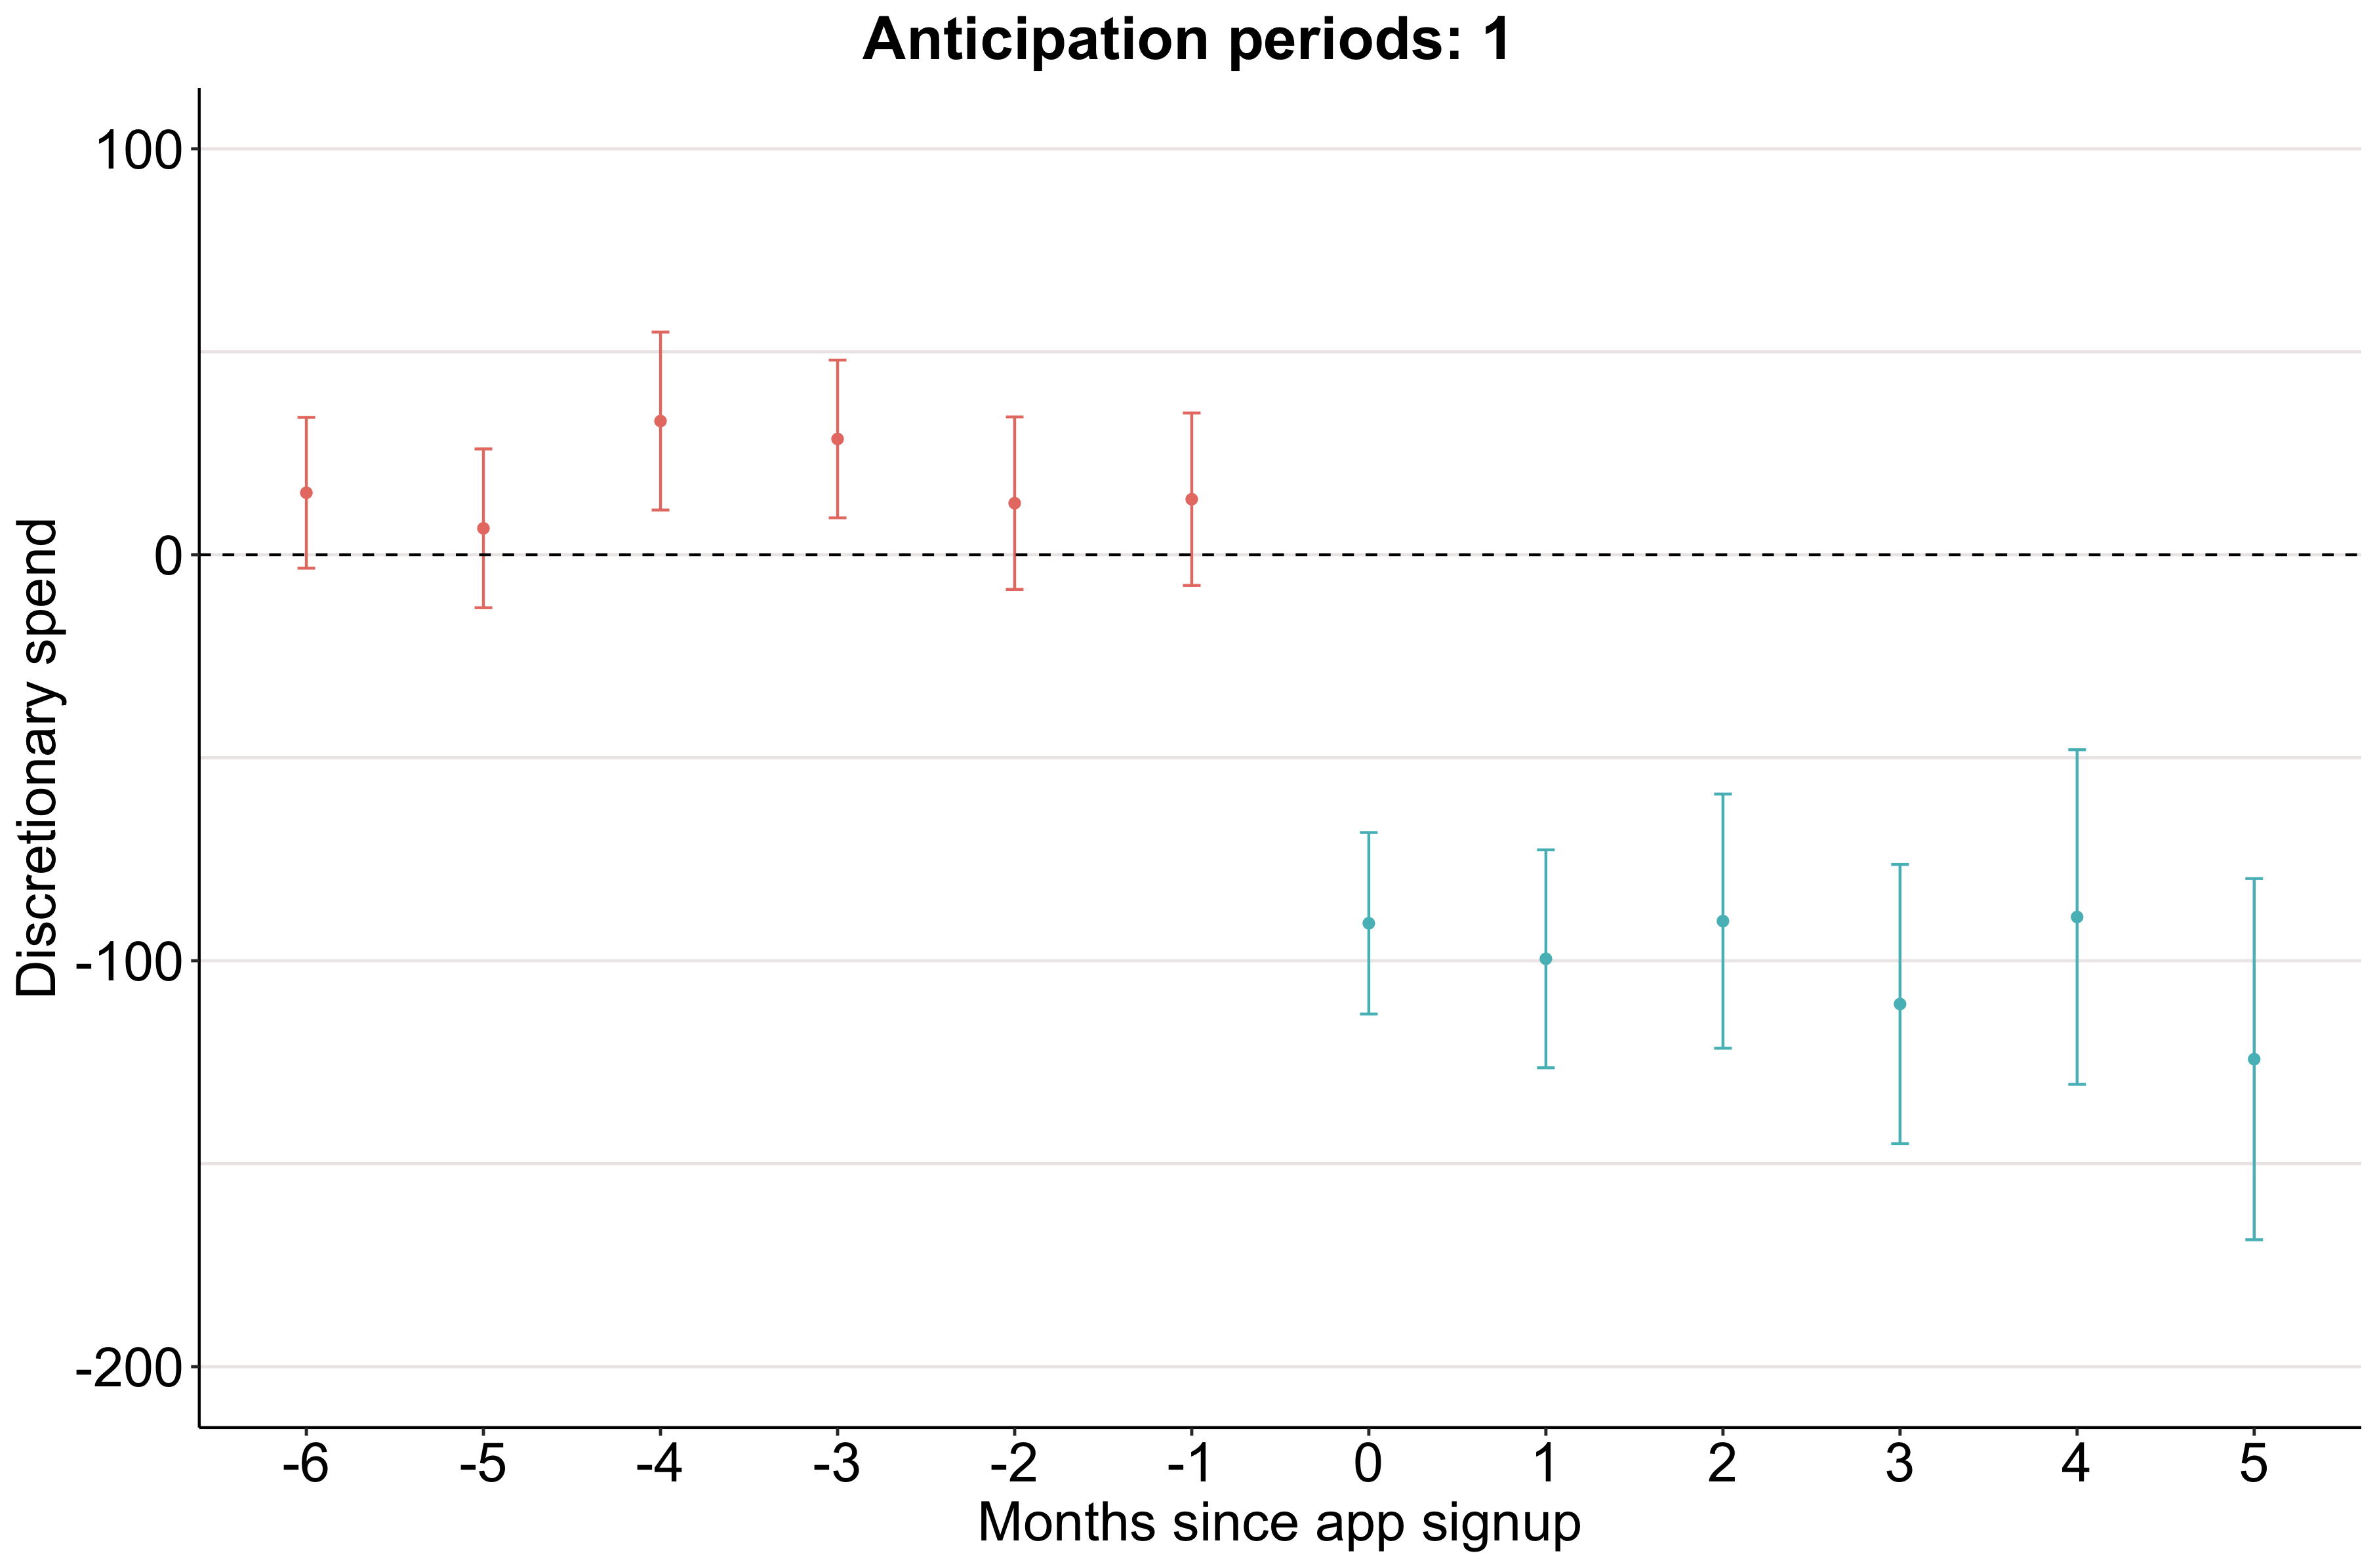
\includegraphics[width=.32\textwidth]{\figdir/dspend_antic1_es.png}
    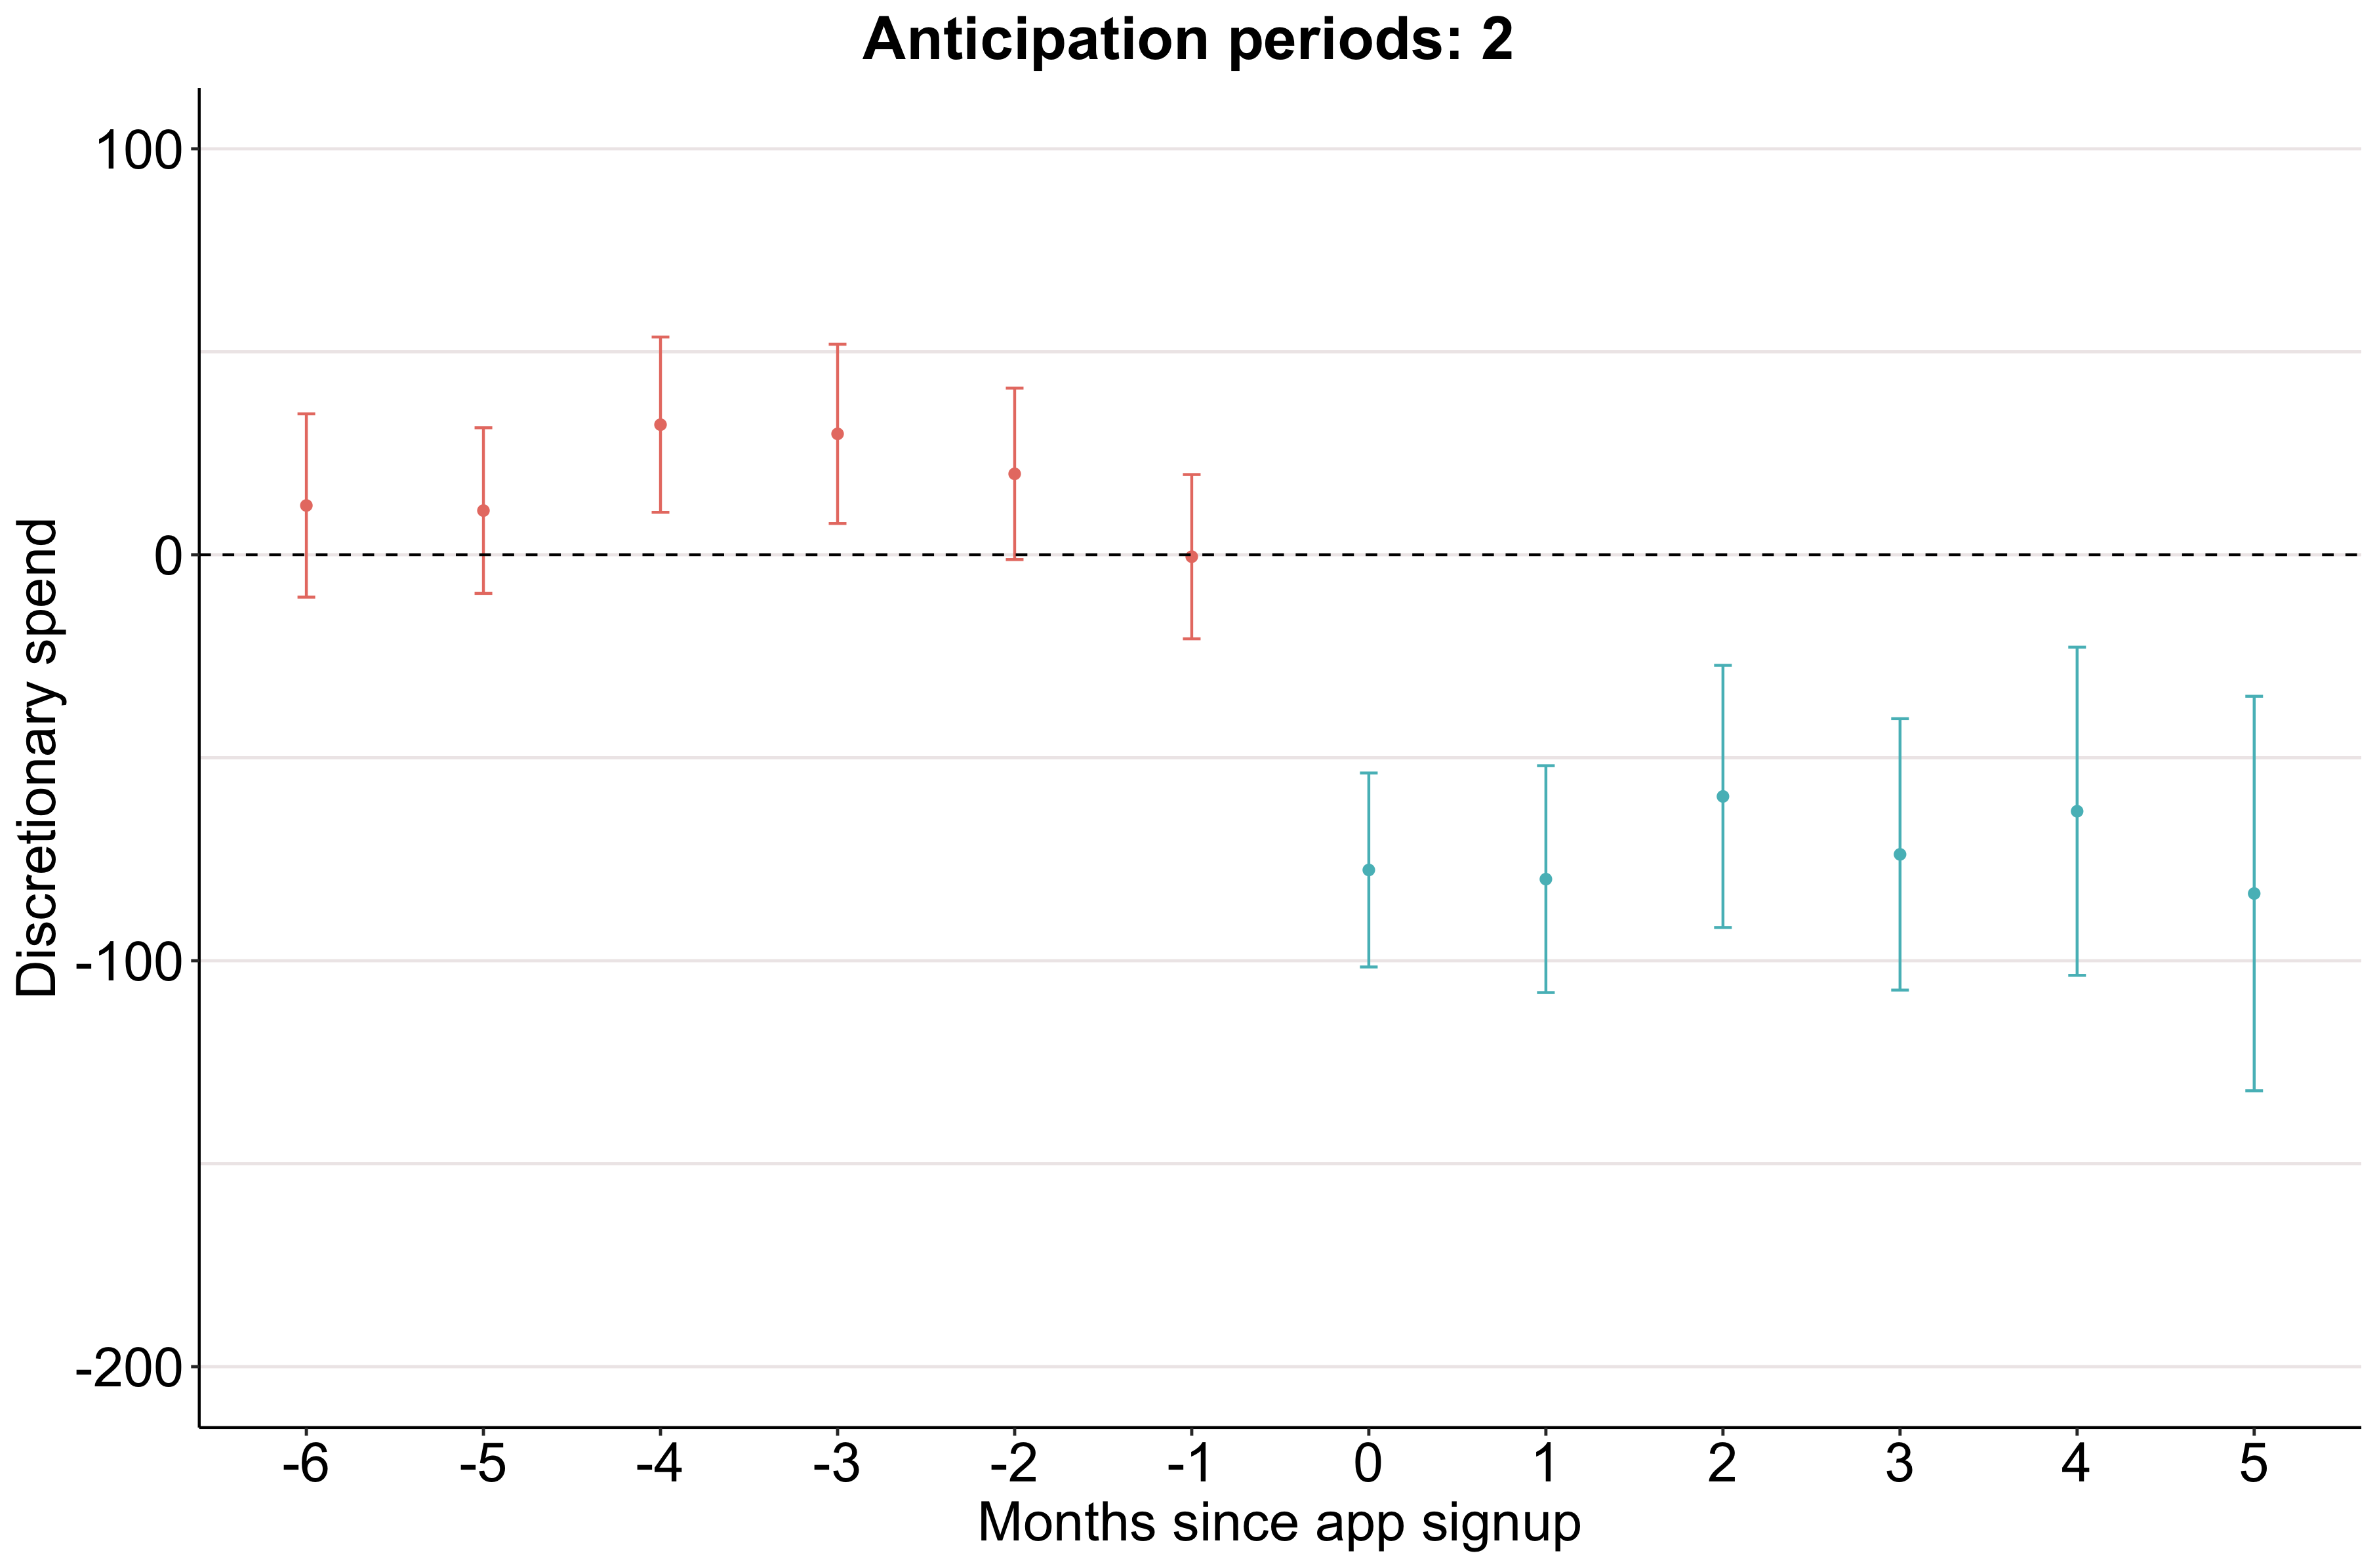
\includegraphics[width=.32\textwidth]{\figdir/dspend_antic2_es.png}
    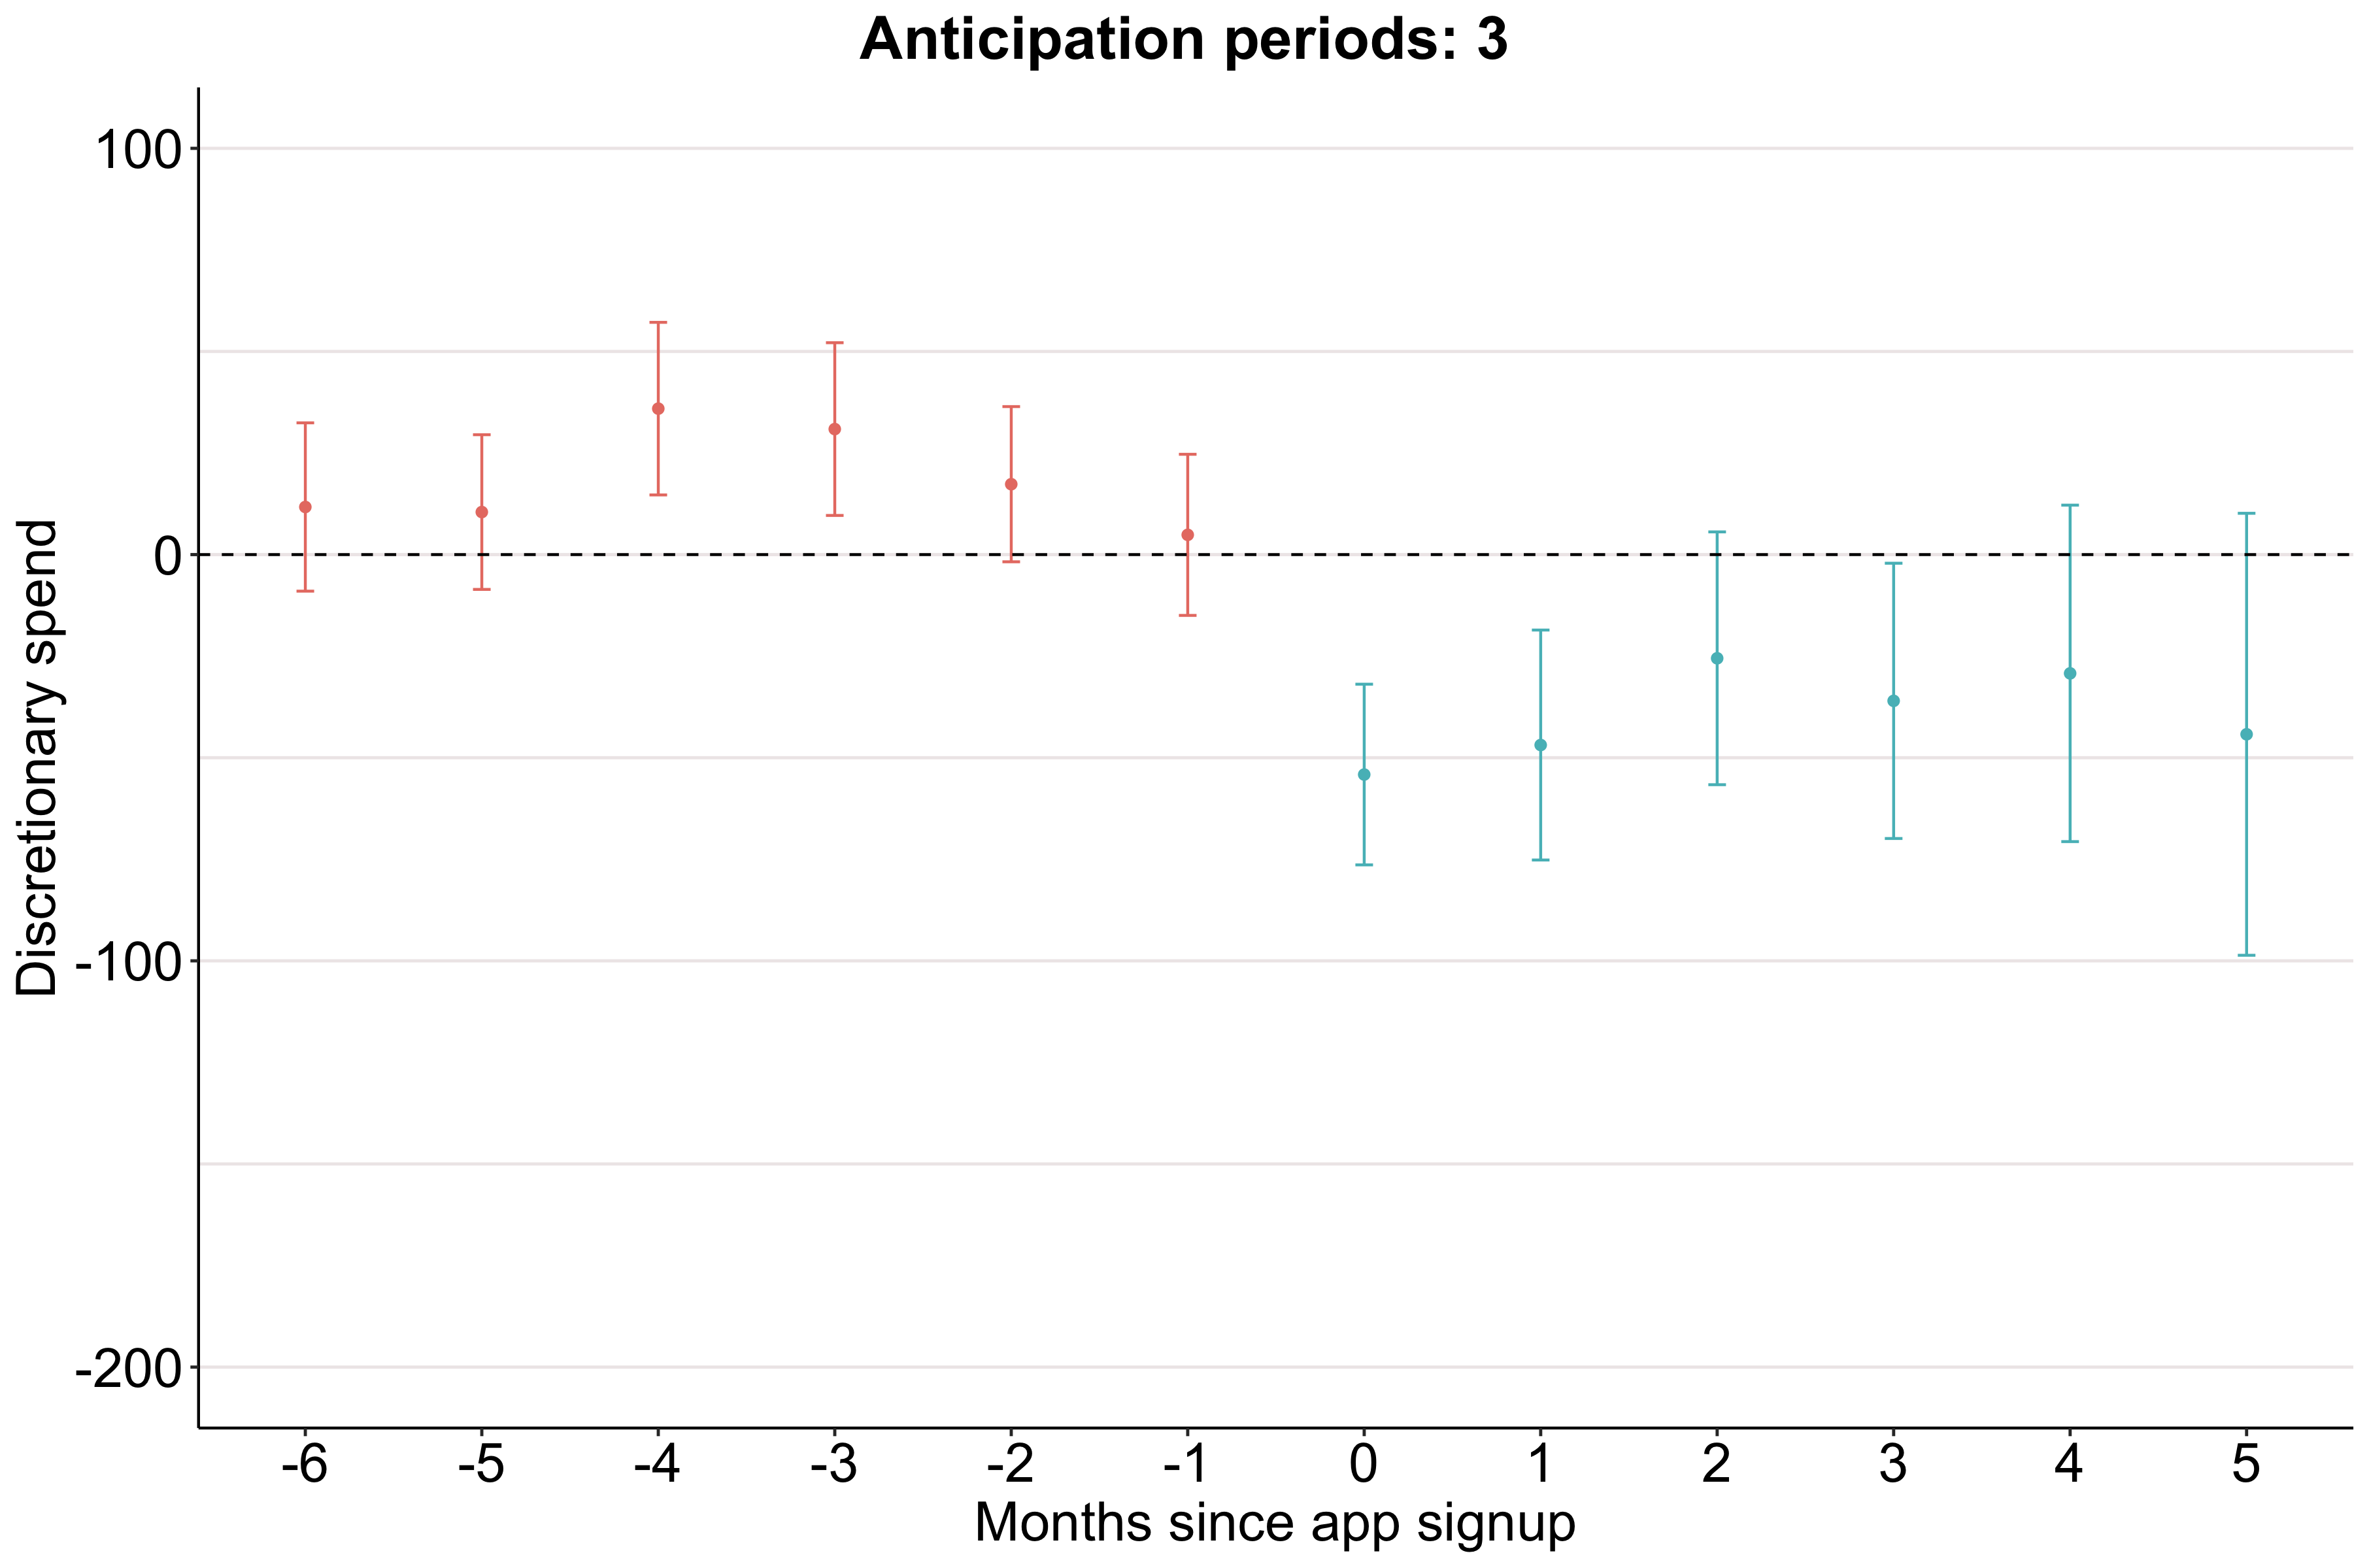
\includegraphics[width=.32\textwidth]{\figdir/dspend_antic3_es.png}
    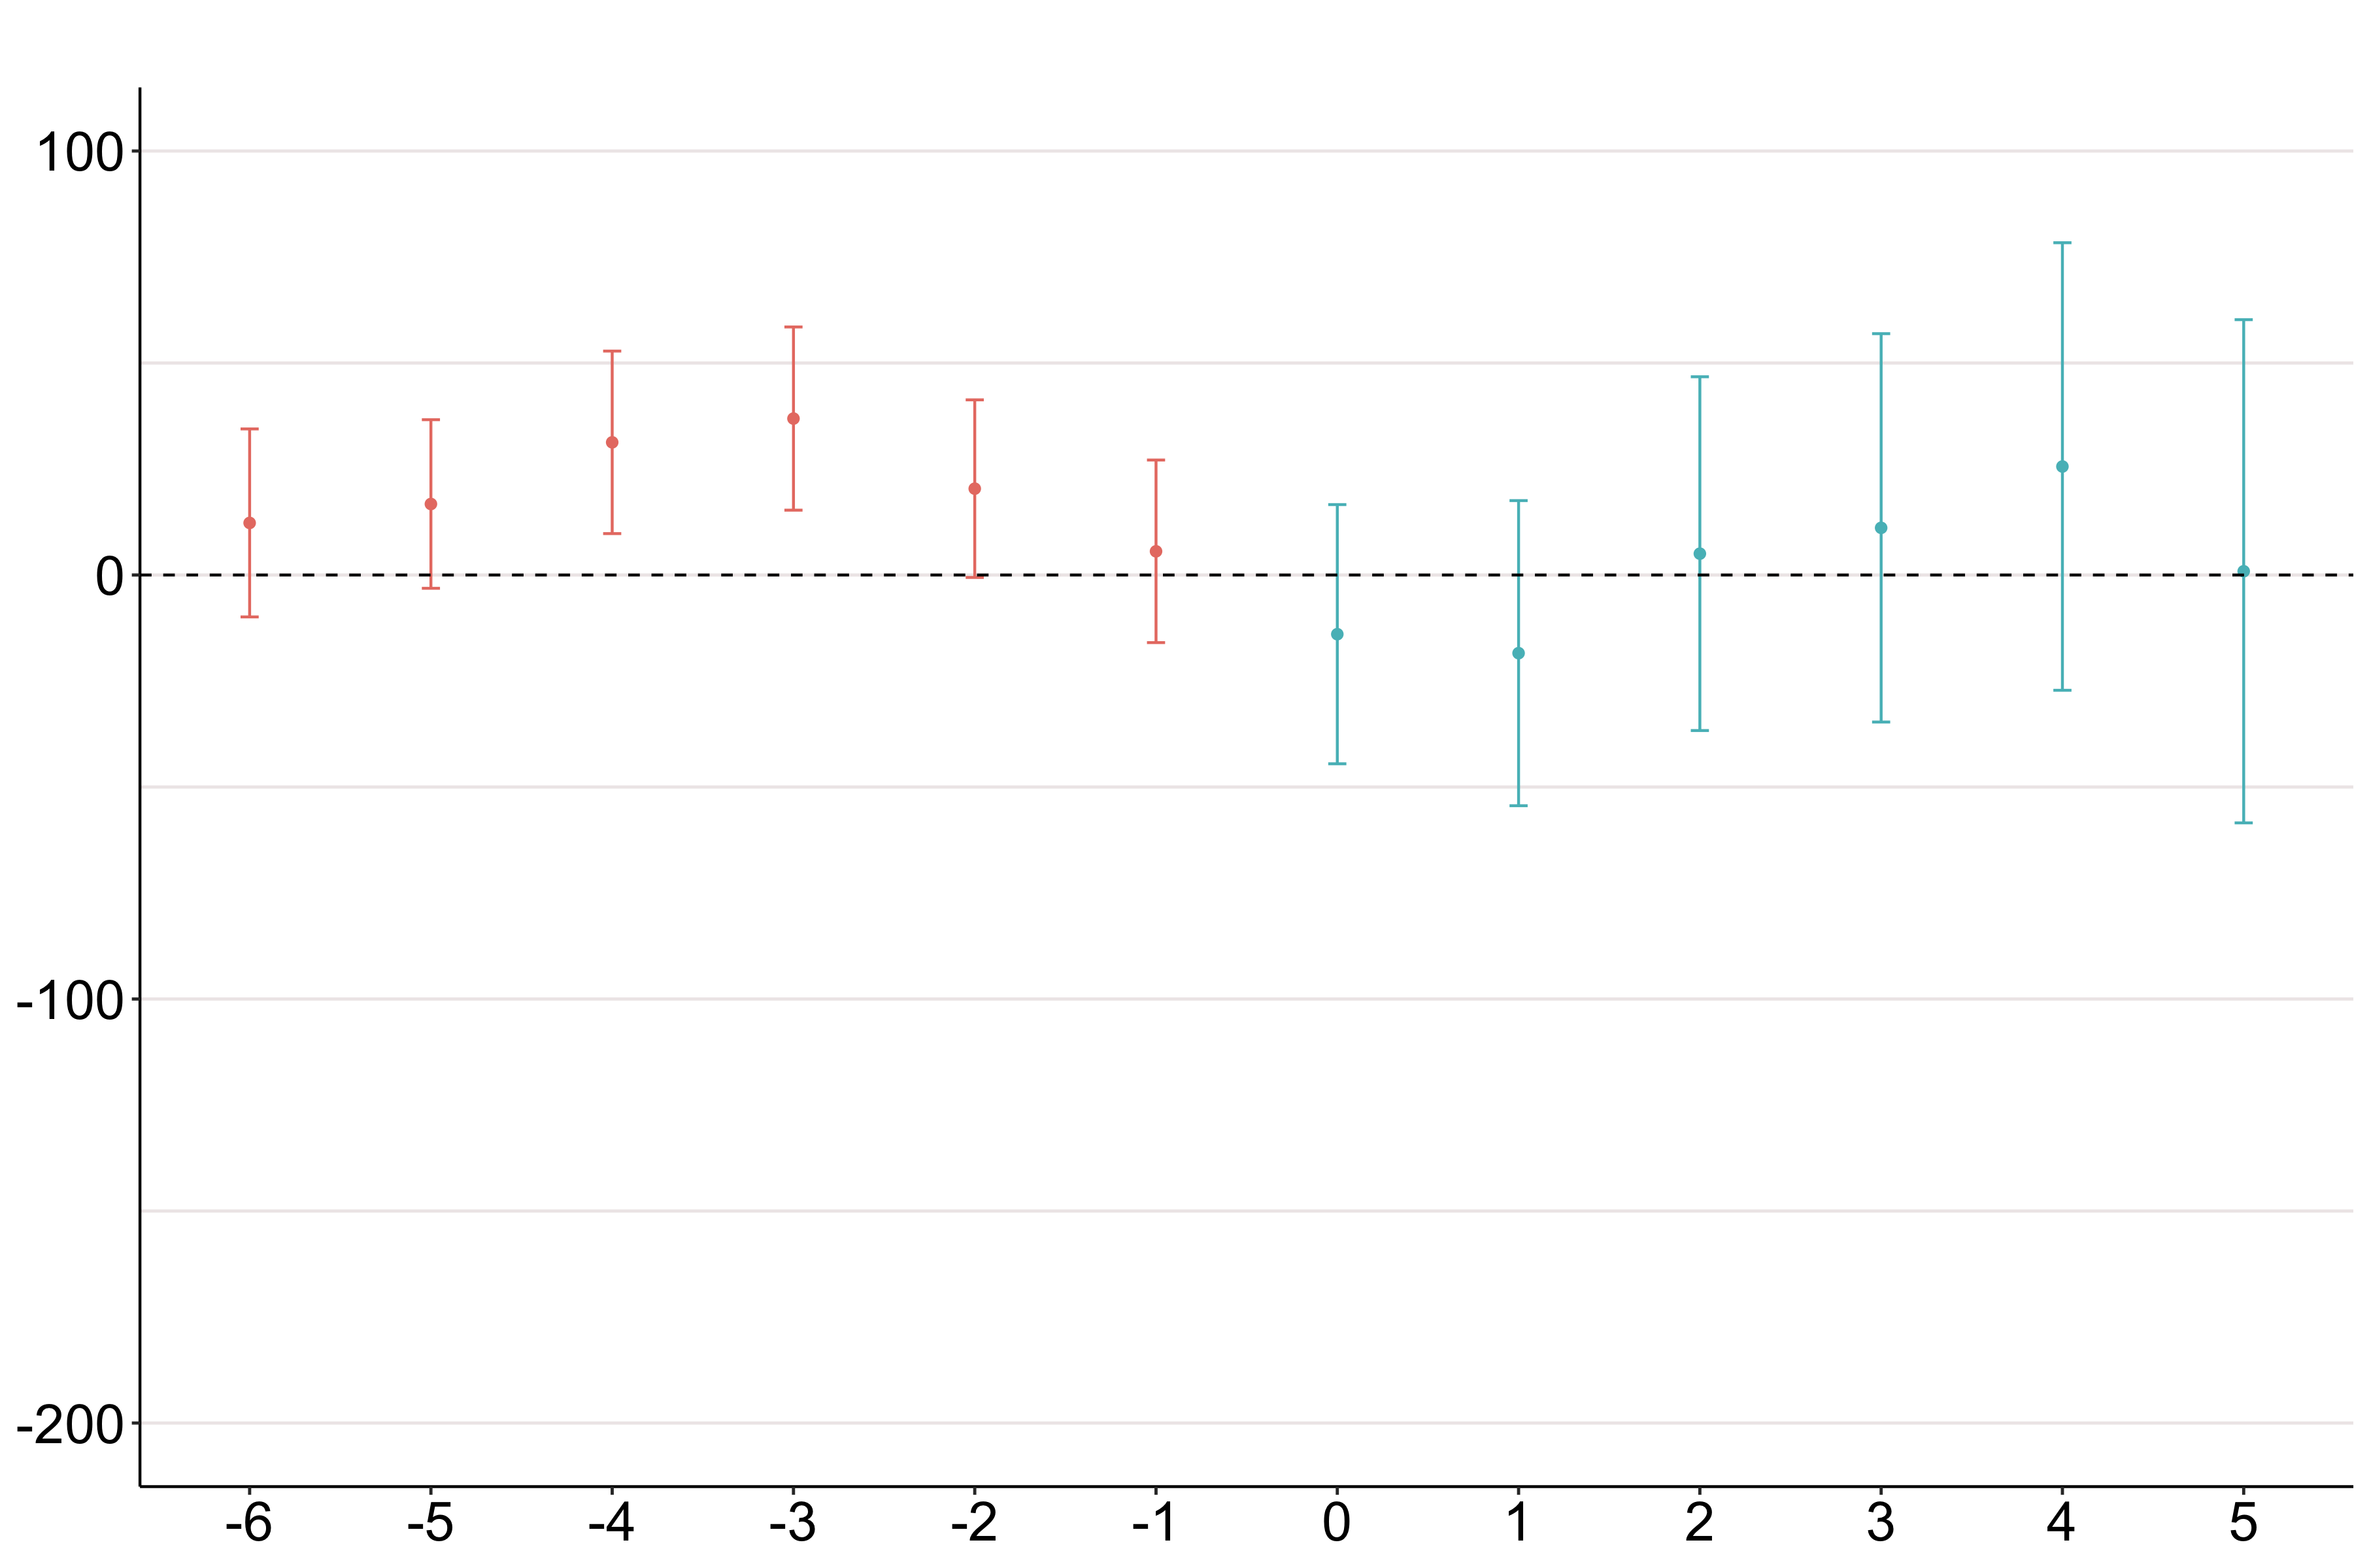
\includegraphics[width=.32\textwidth]{\figdir/dspend_antic4_es.png}
    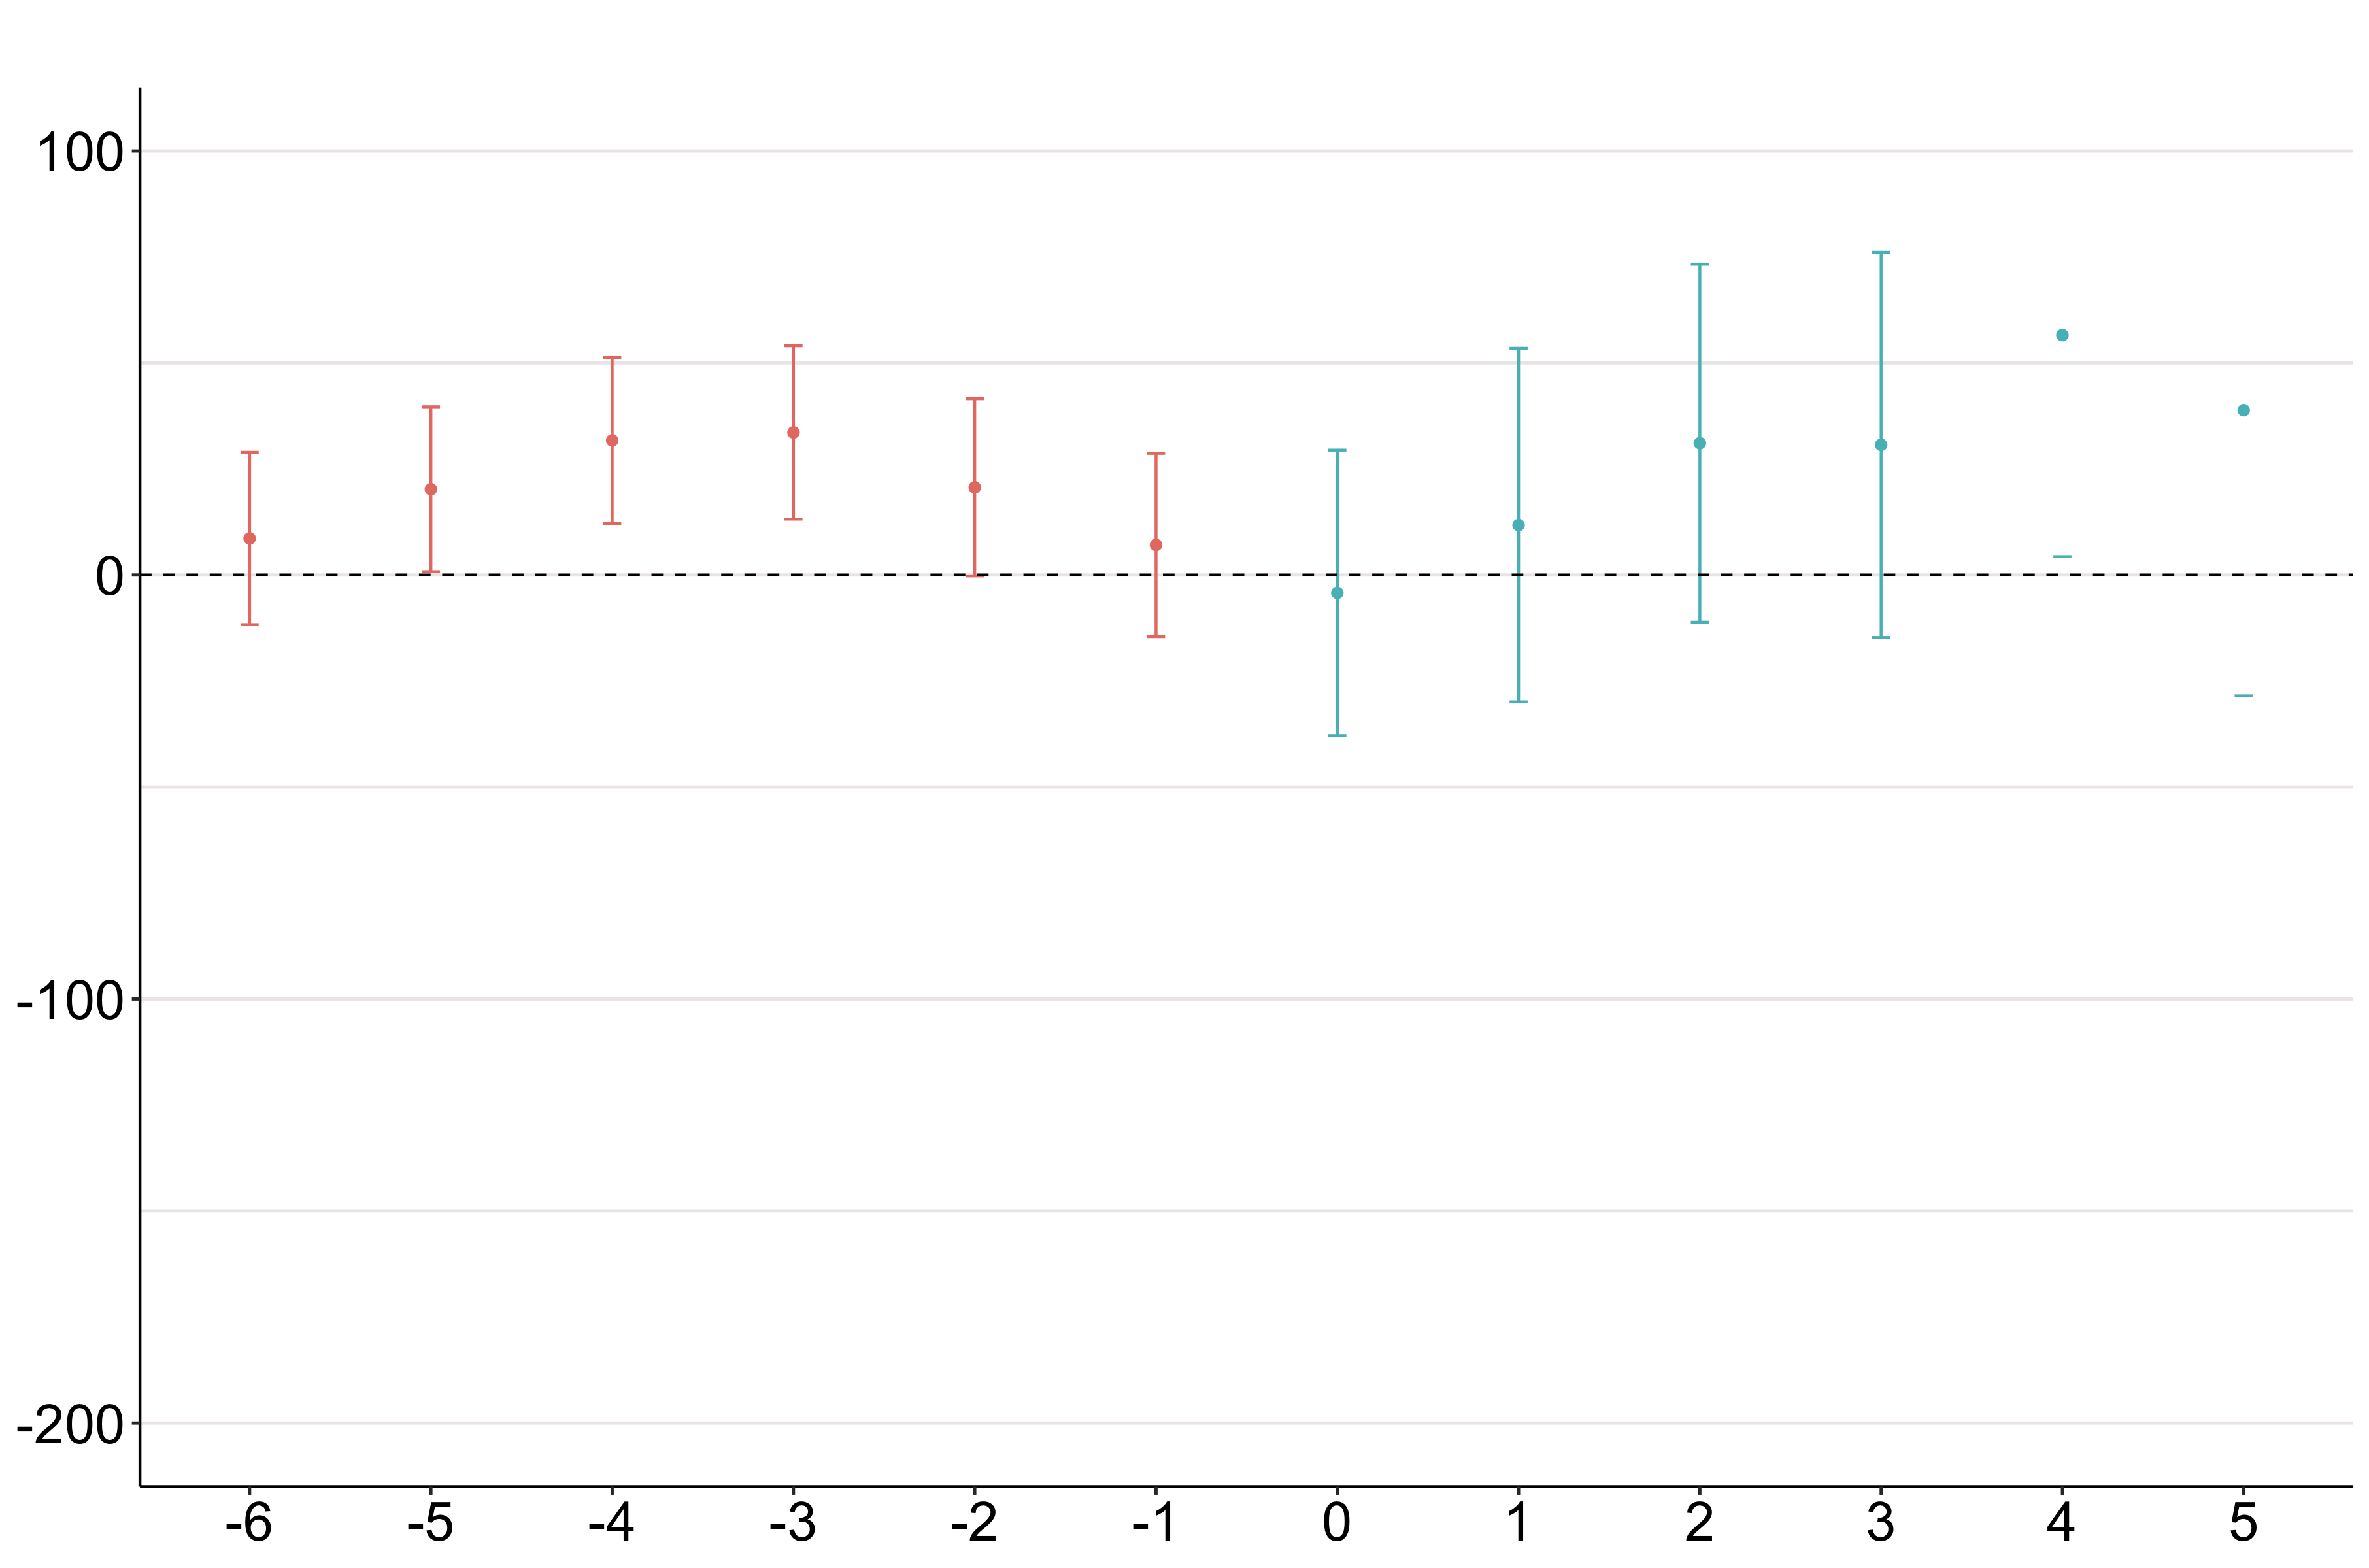
\includegraphics[width=.32\textwidth]{\figdir/dspend_antic5_es.png}
    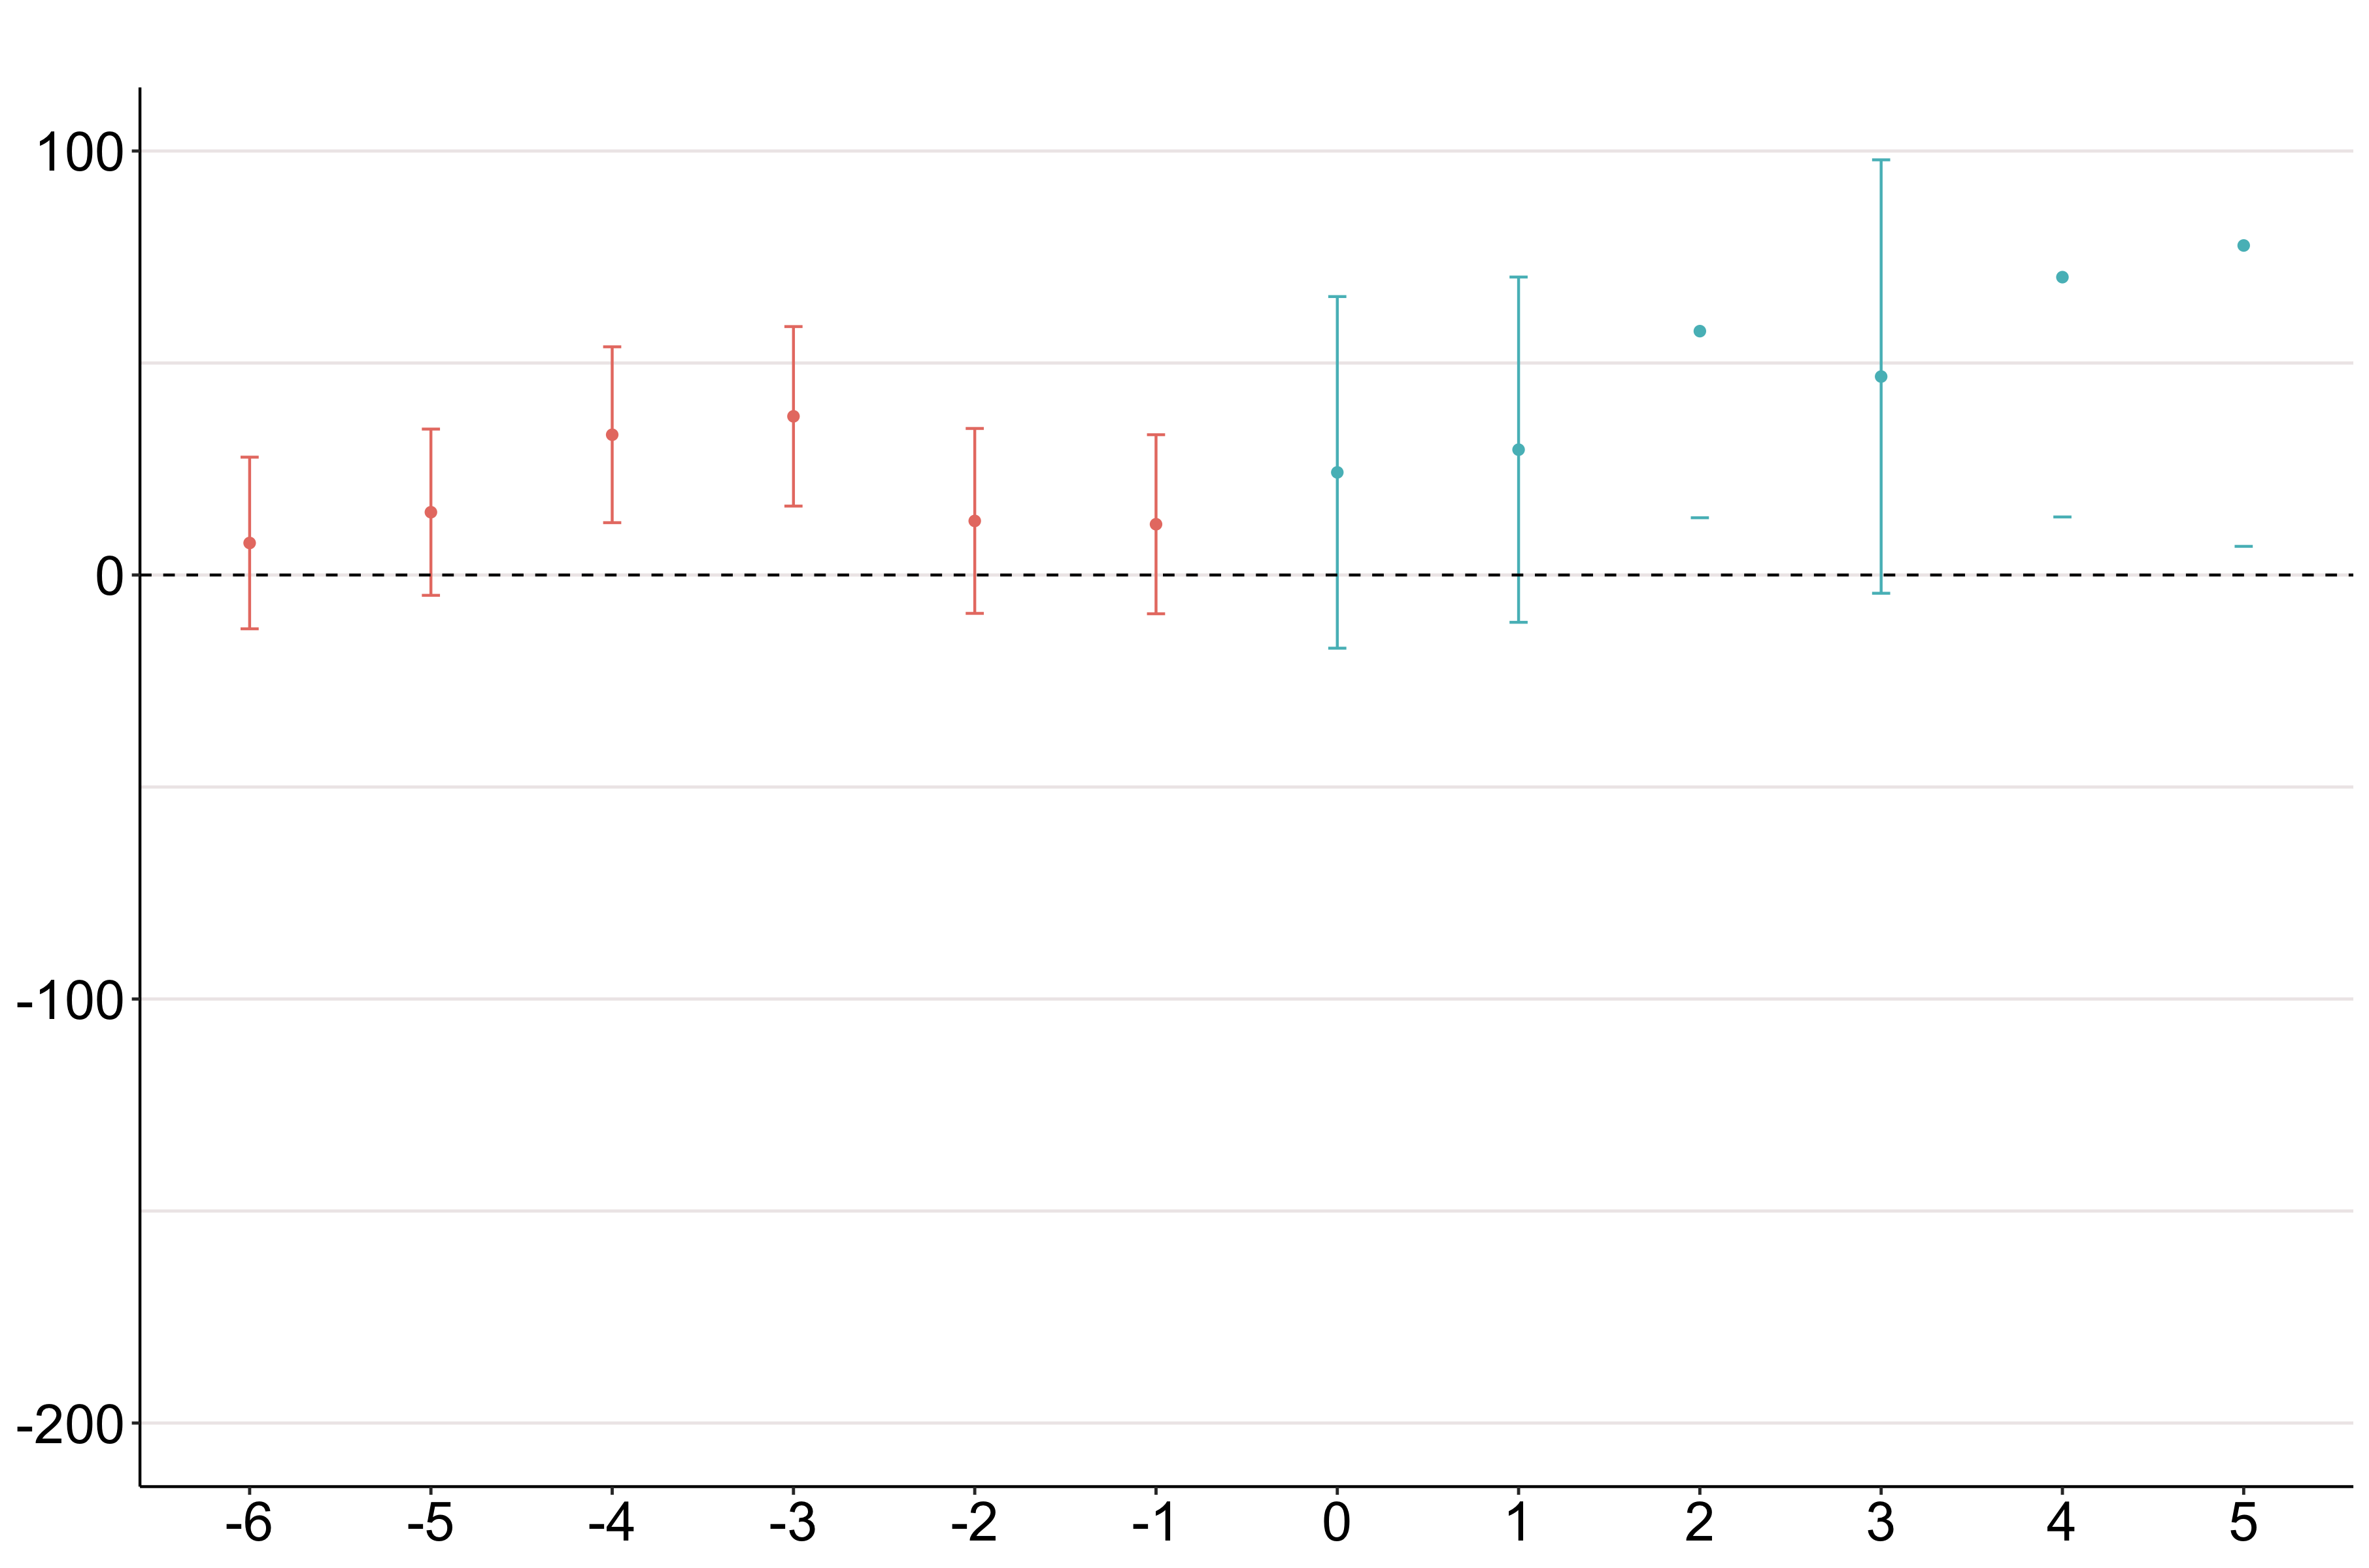
\includegraphics[width=.32\textwidth]{\figdir/dspend_antic6_es.png}
    \fignote{\textwidth}{...}
\end{figure}

\begin{figure}[H]
    \centering
    \caption{Anticipation ...}%
    \label{fig:new}
    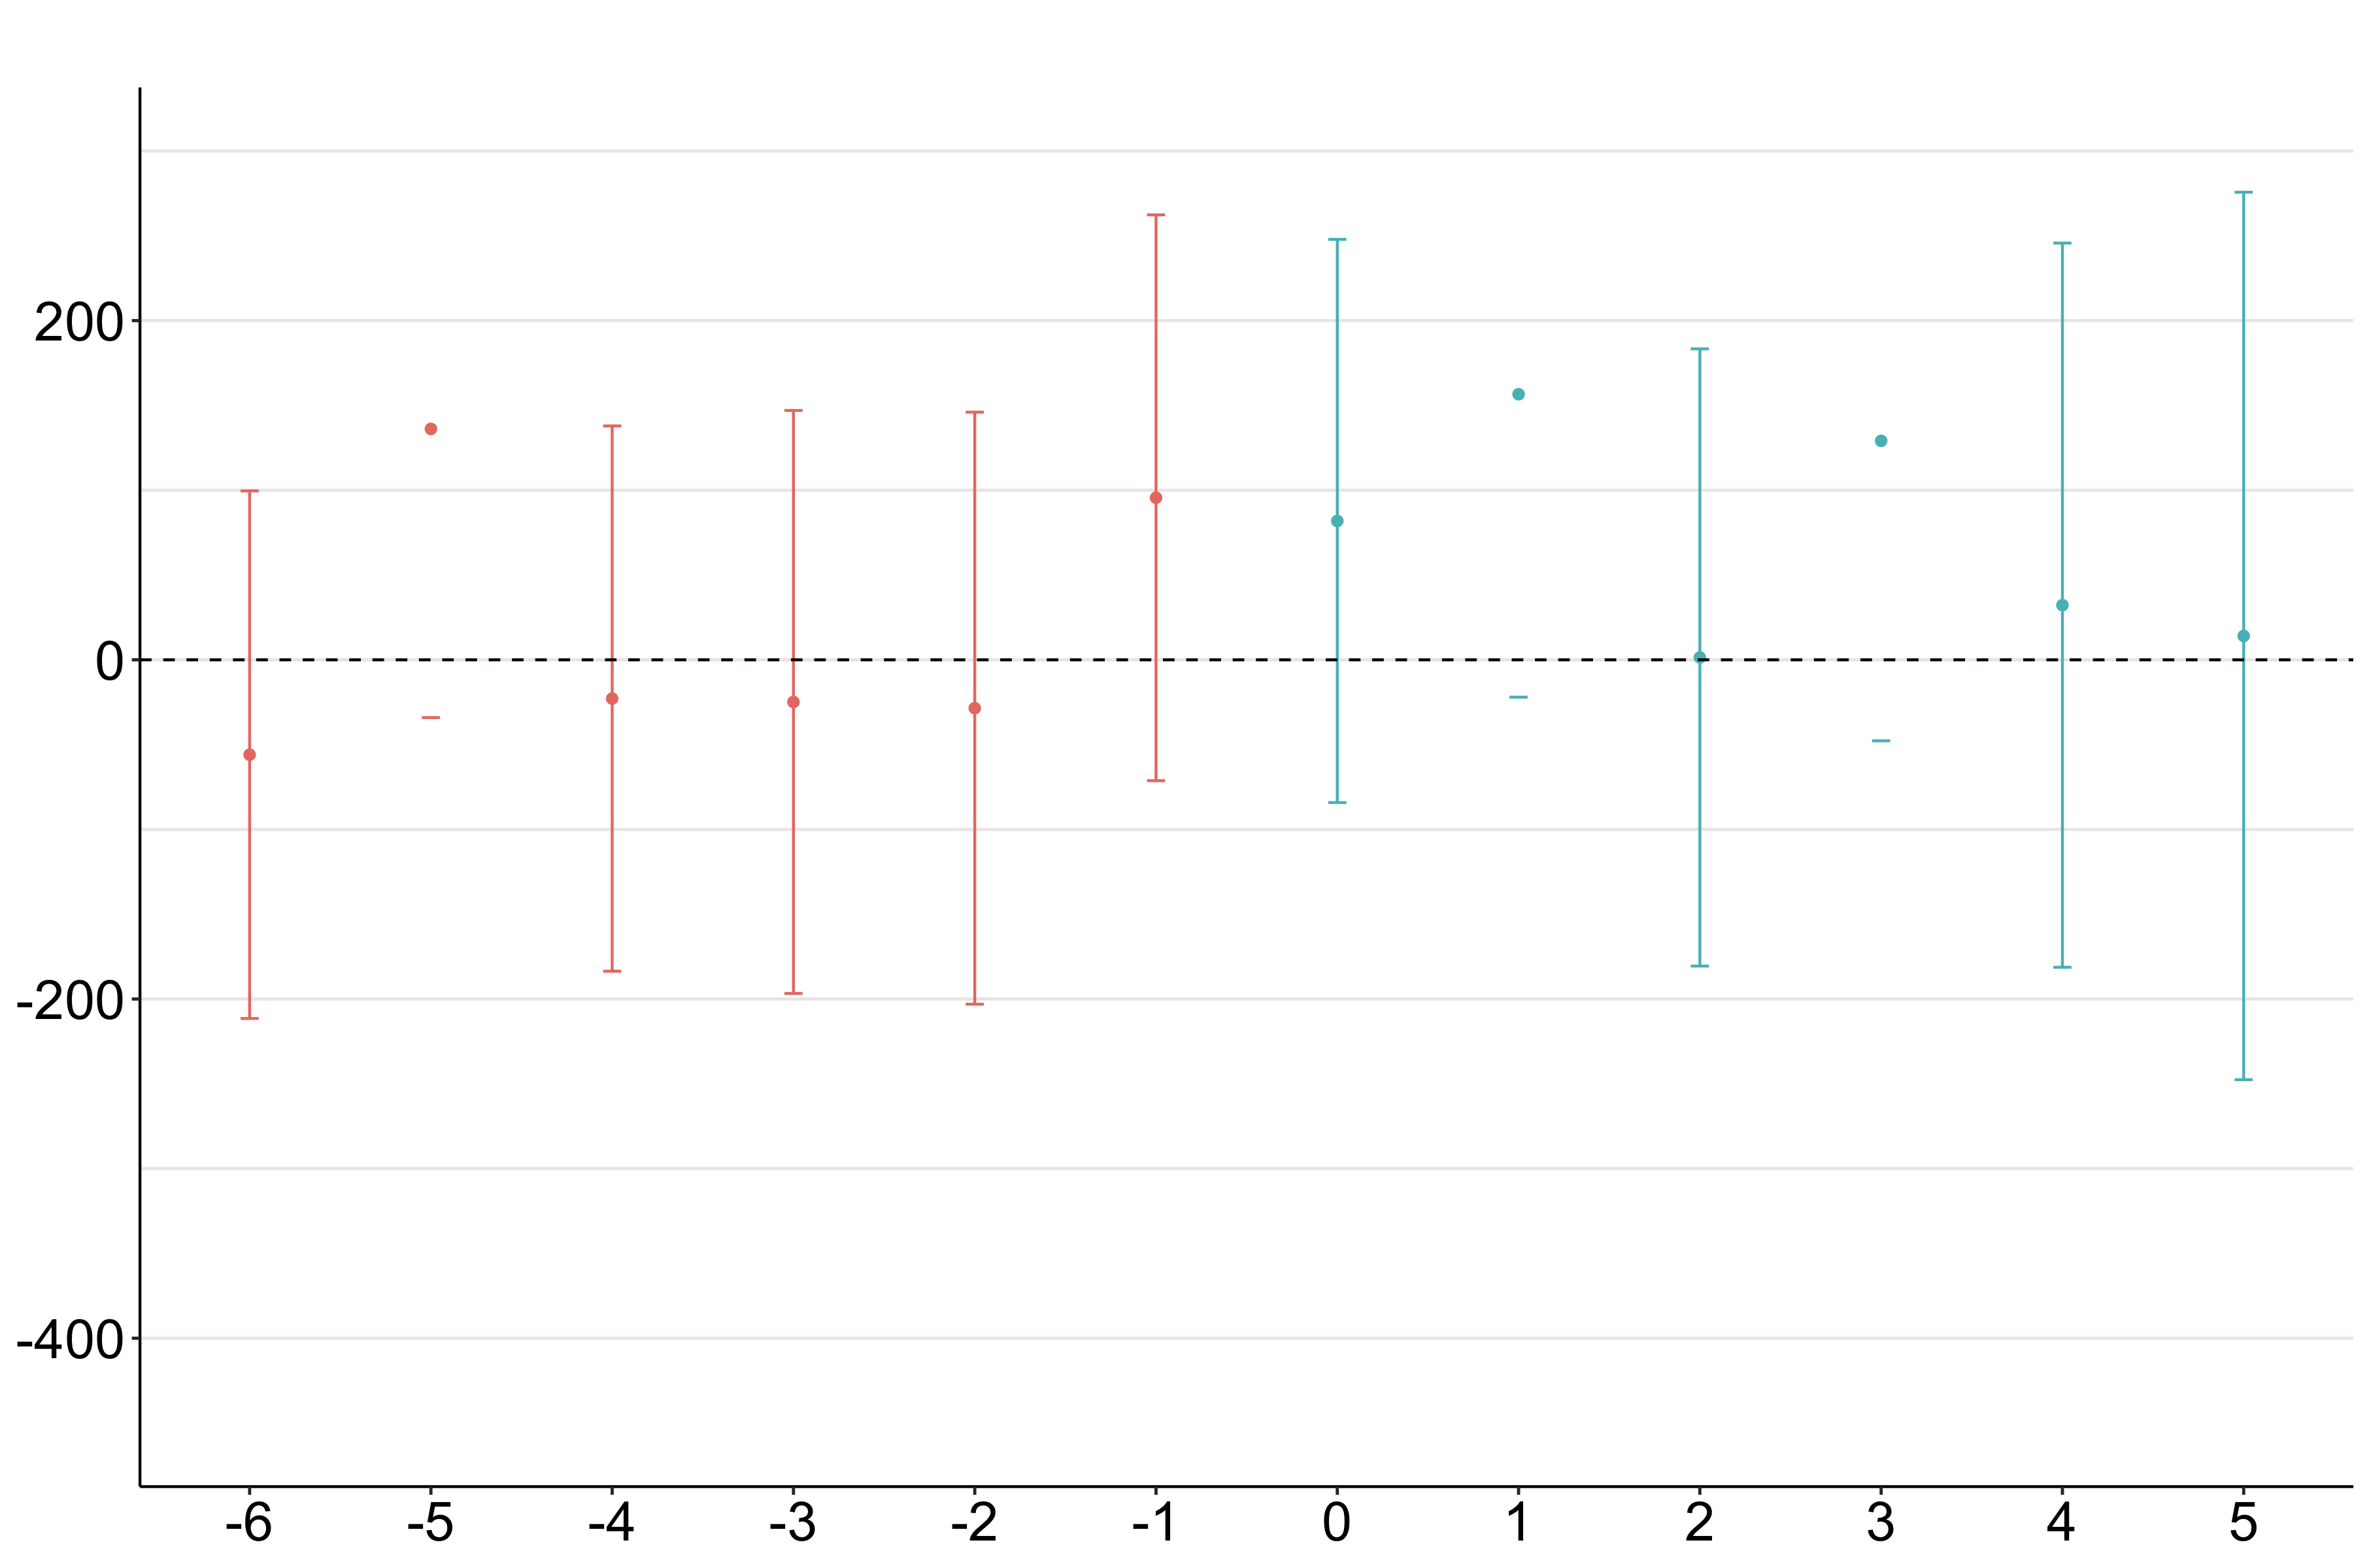
\includegraphics[width=.32\textwidth]{\figdir/netflows_antic1_es.png}
    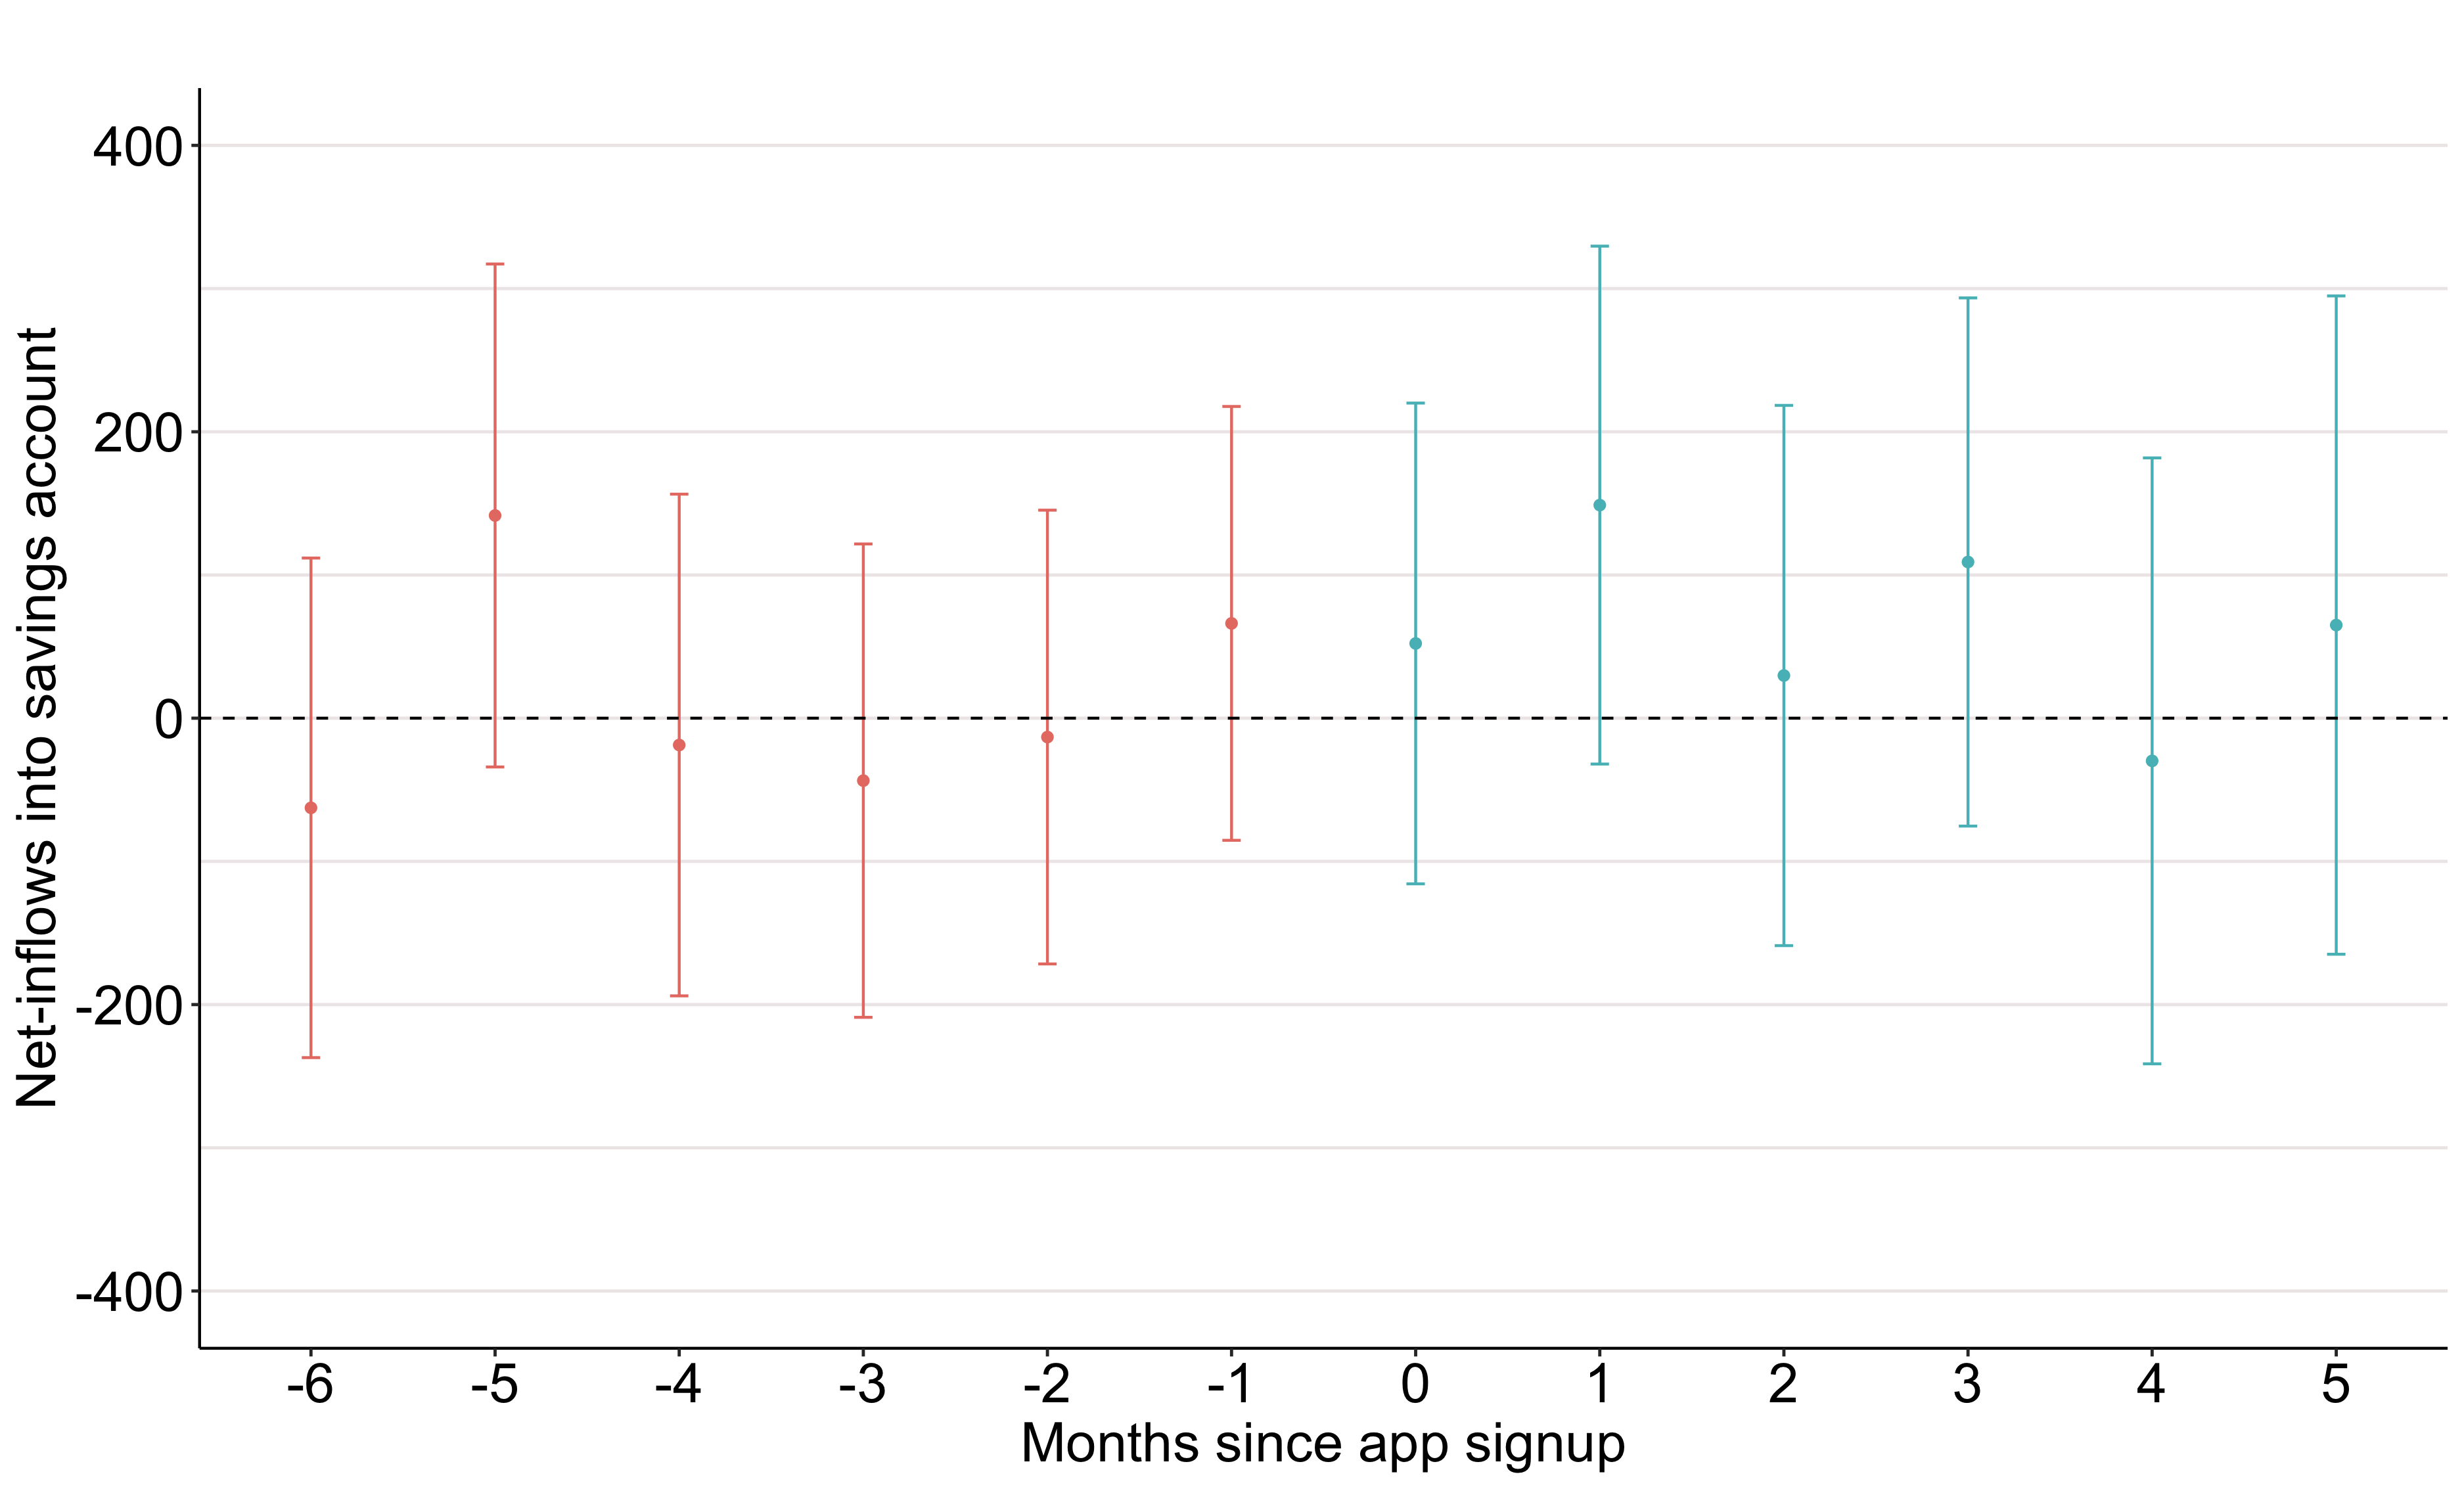
\includegraphics[width=.32\textwidth]{\figdir/netflows_antic2_es.png}
    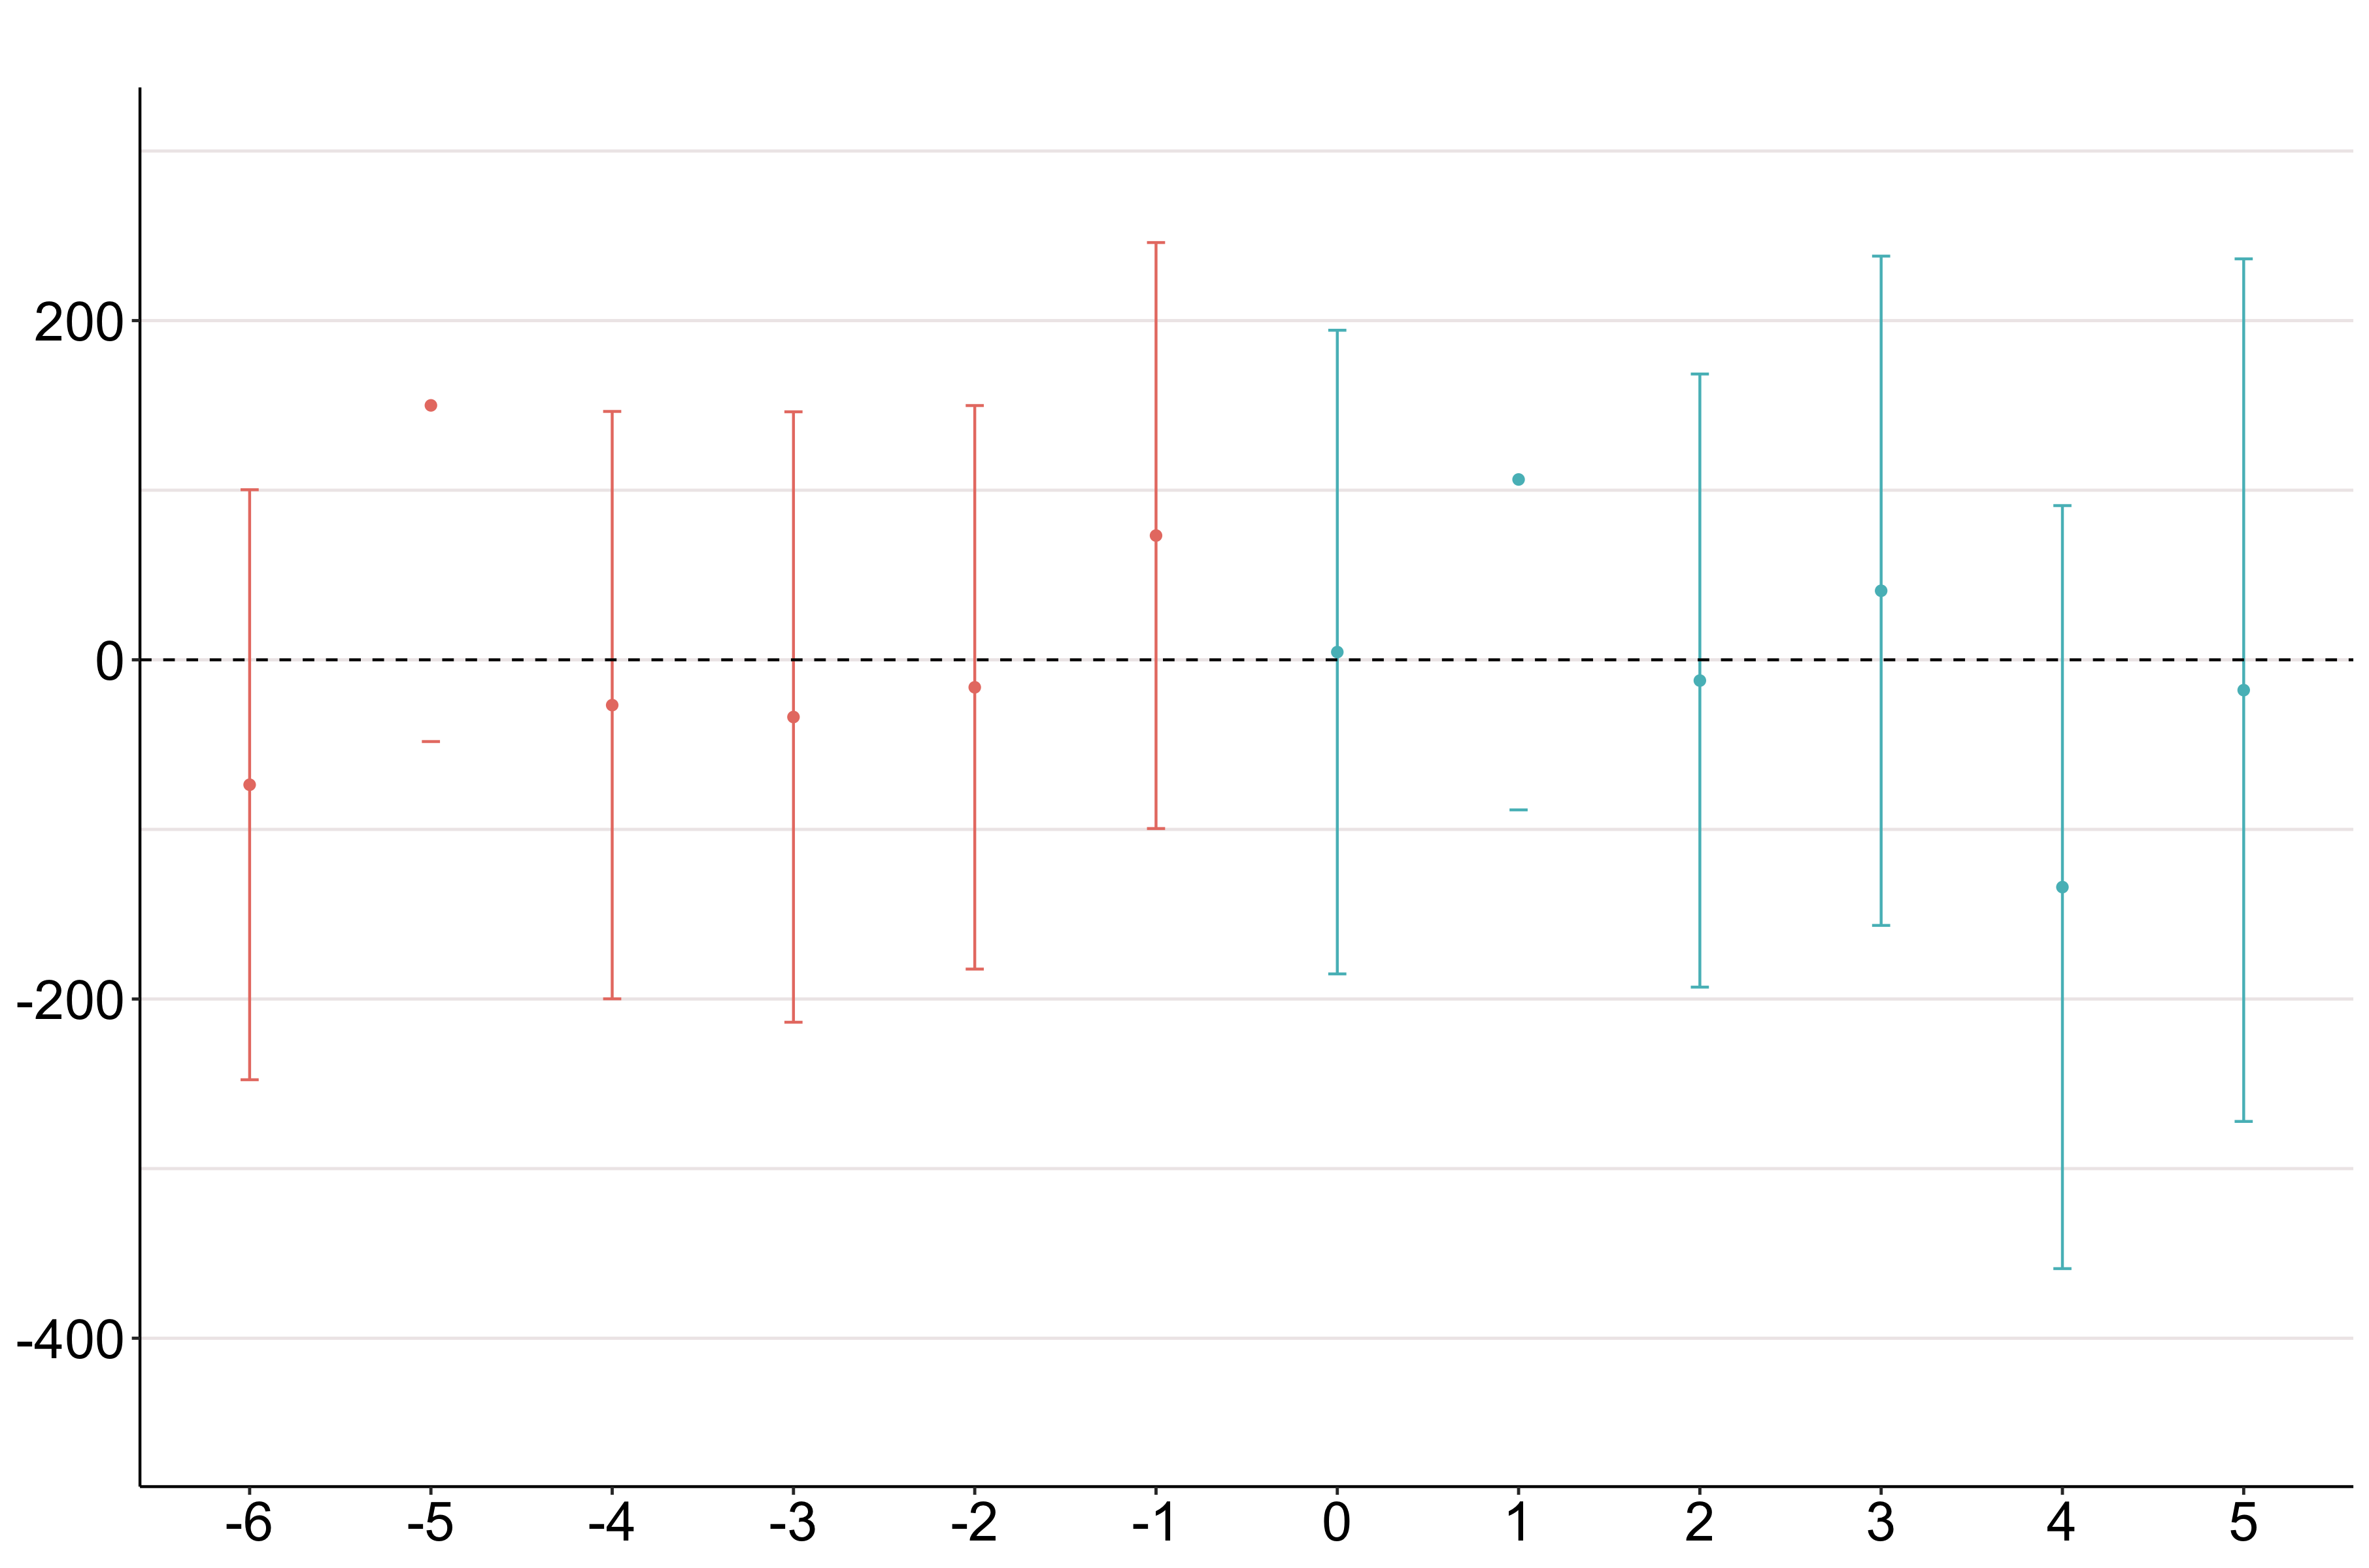
\includegraphics[width=.32\textwidth]{\figdir/netflows_antic3_es.png}
    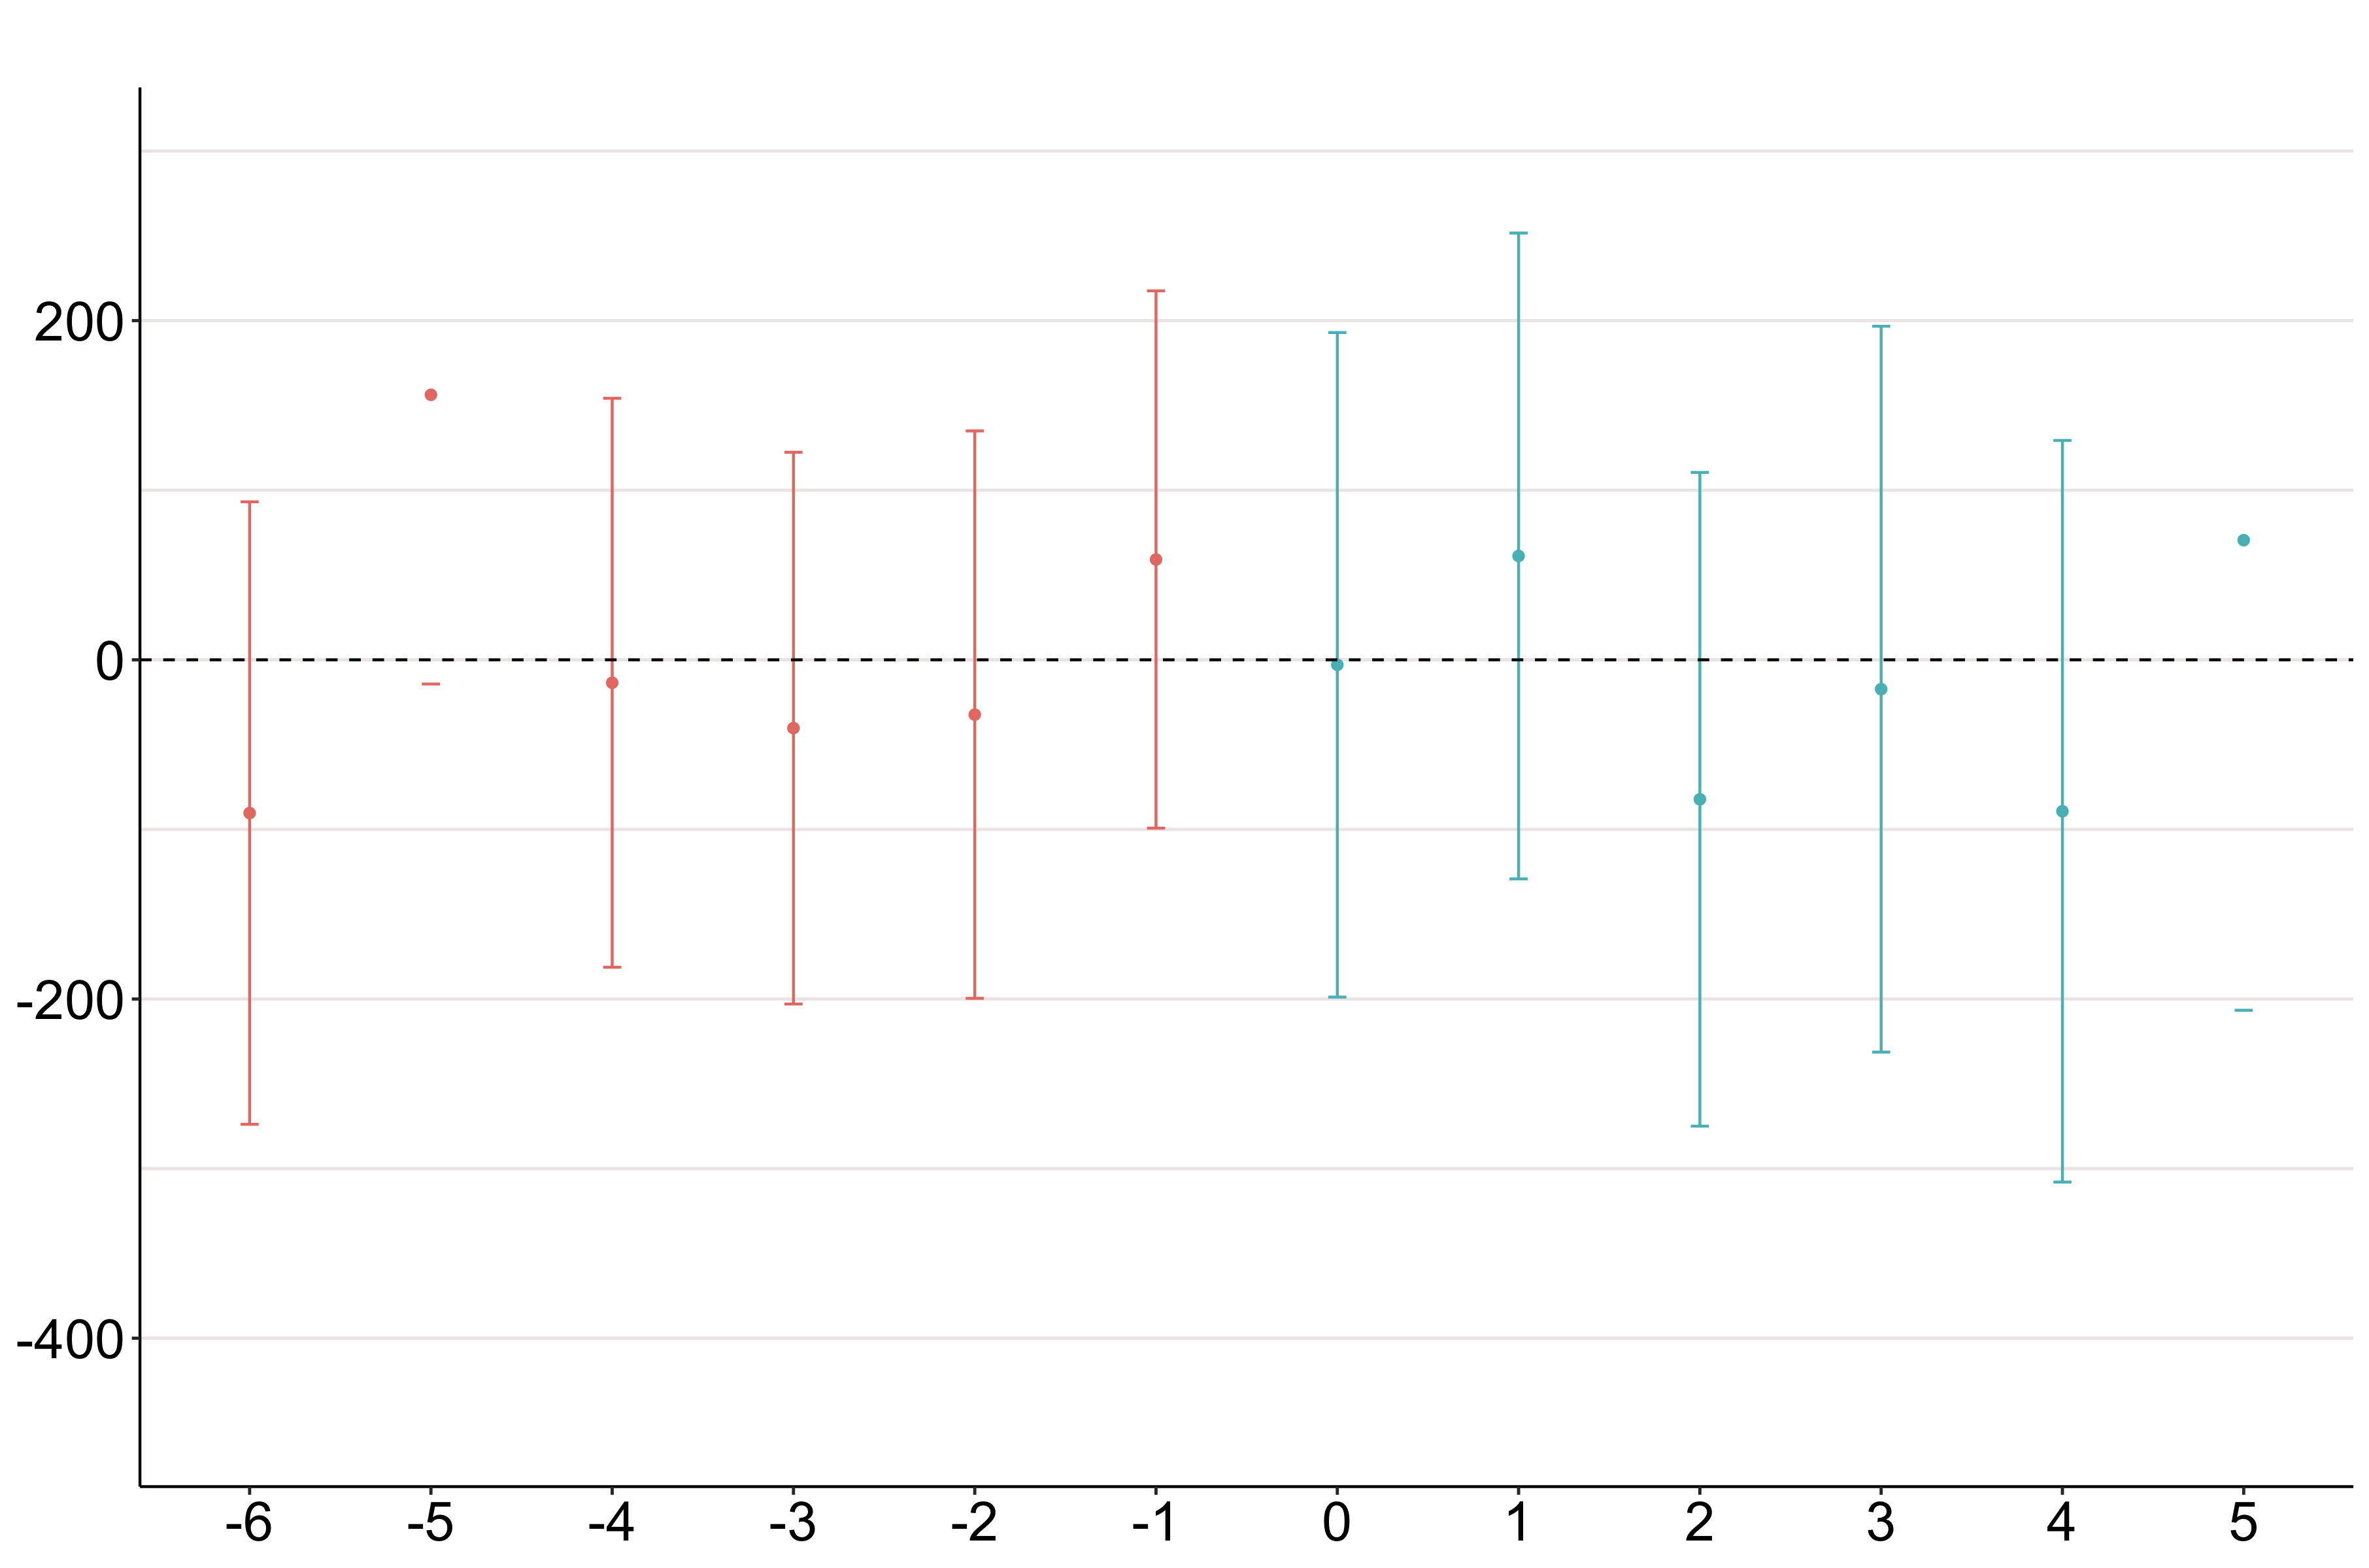
\includegraphics[width=.32\textwidth]{\figdir/netflows_antic4_es.png}
    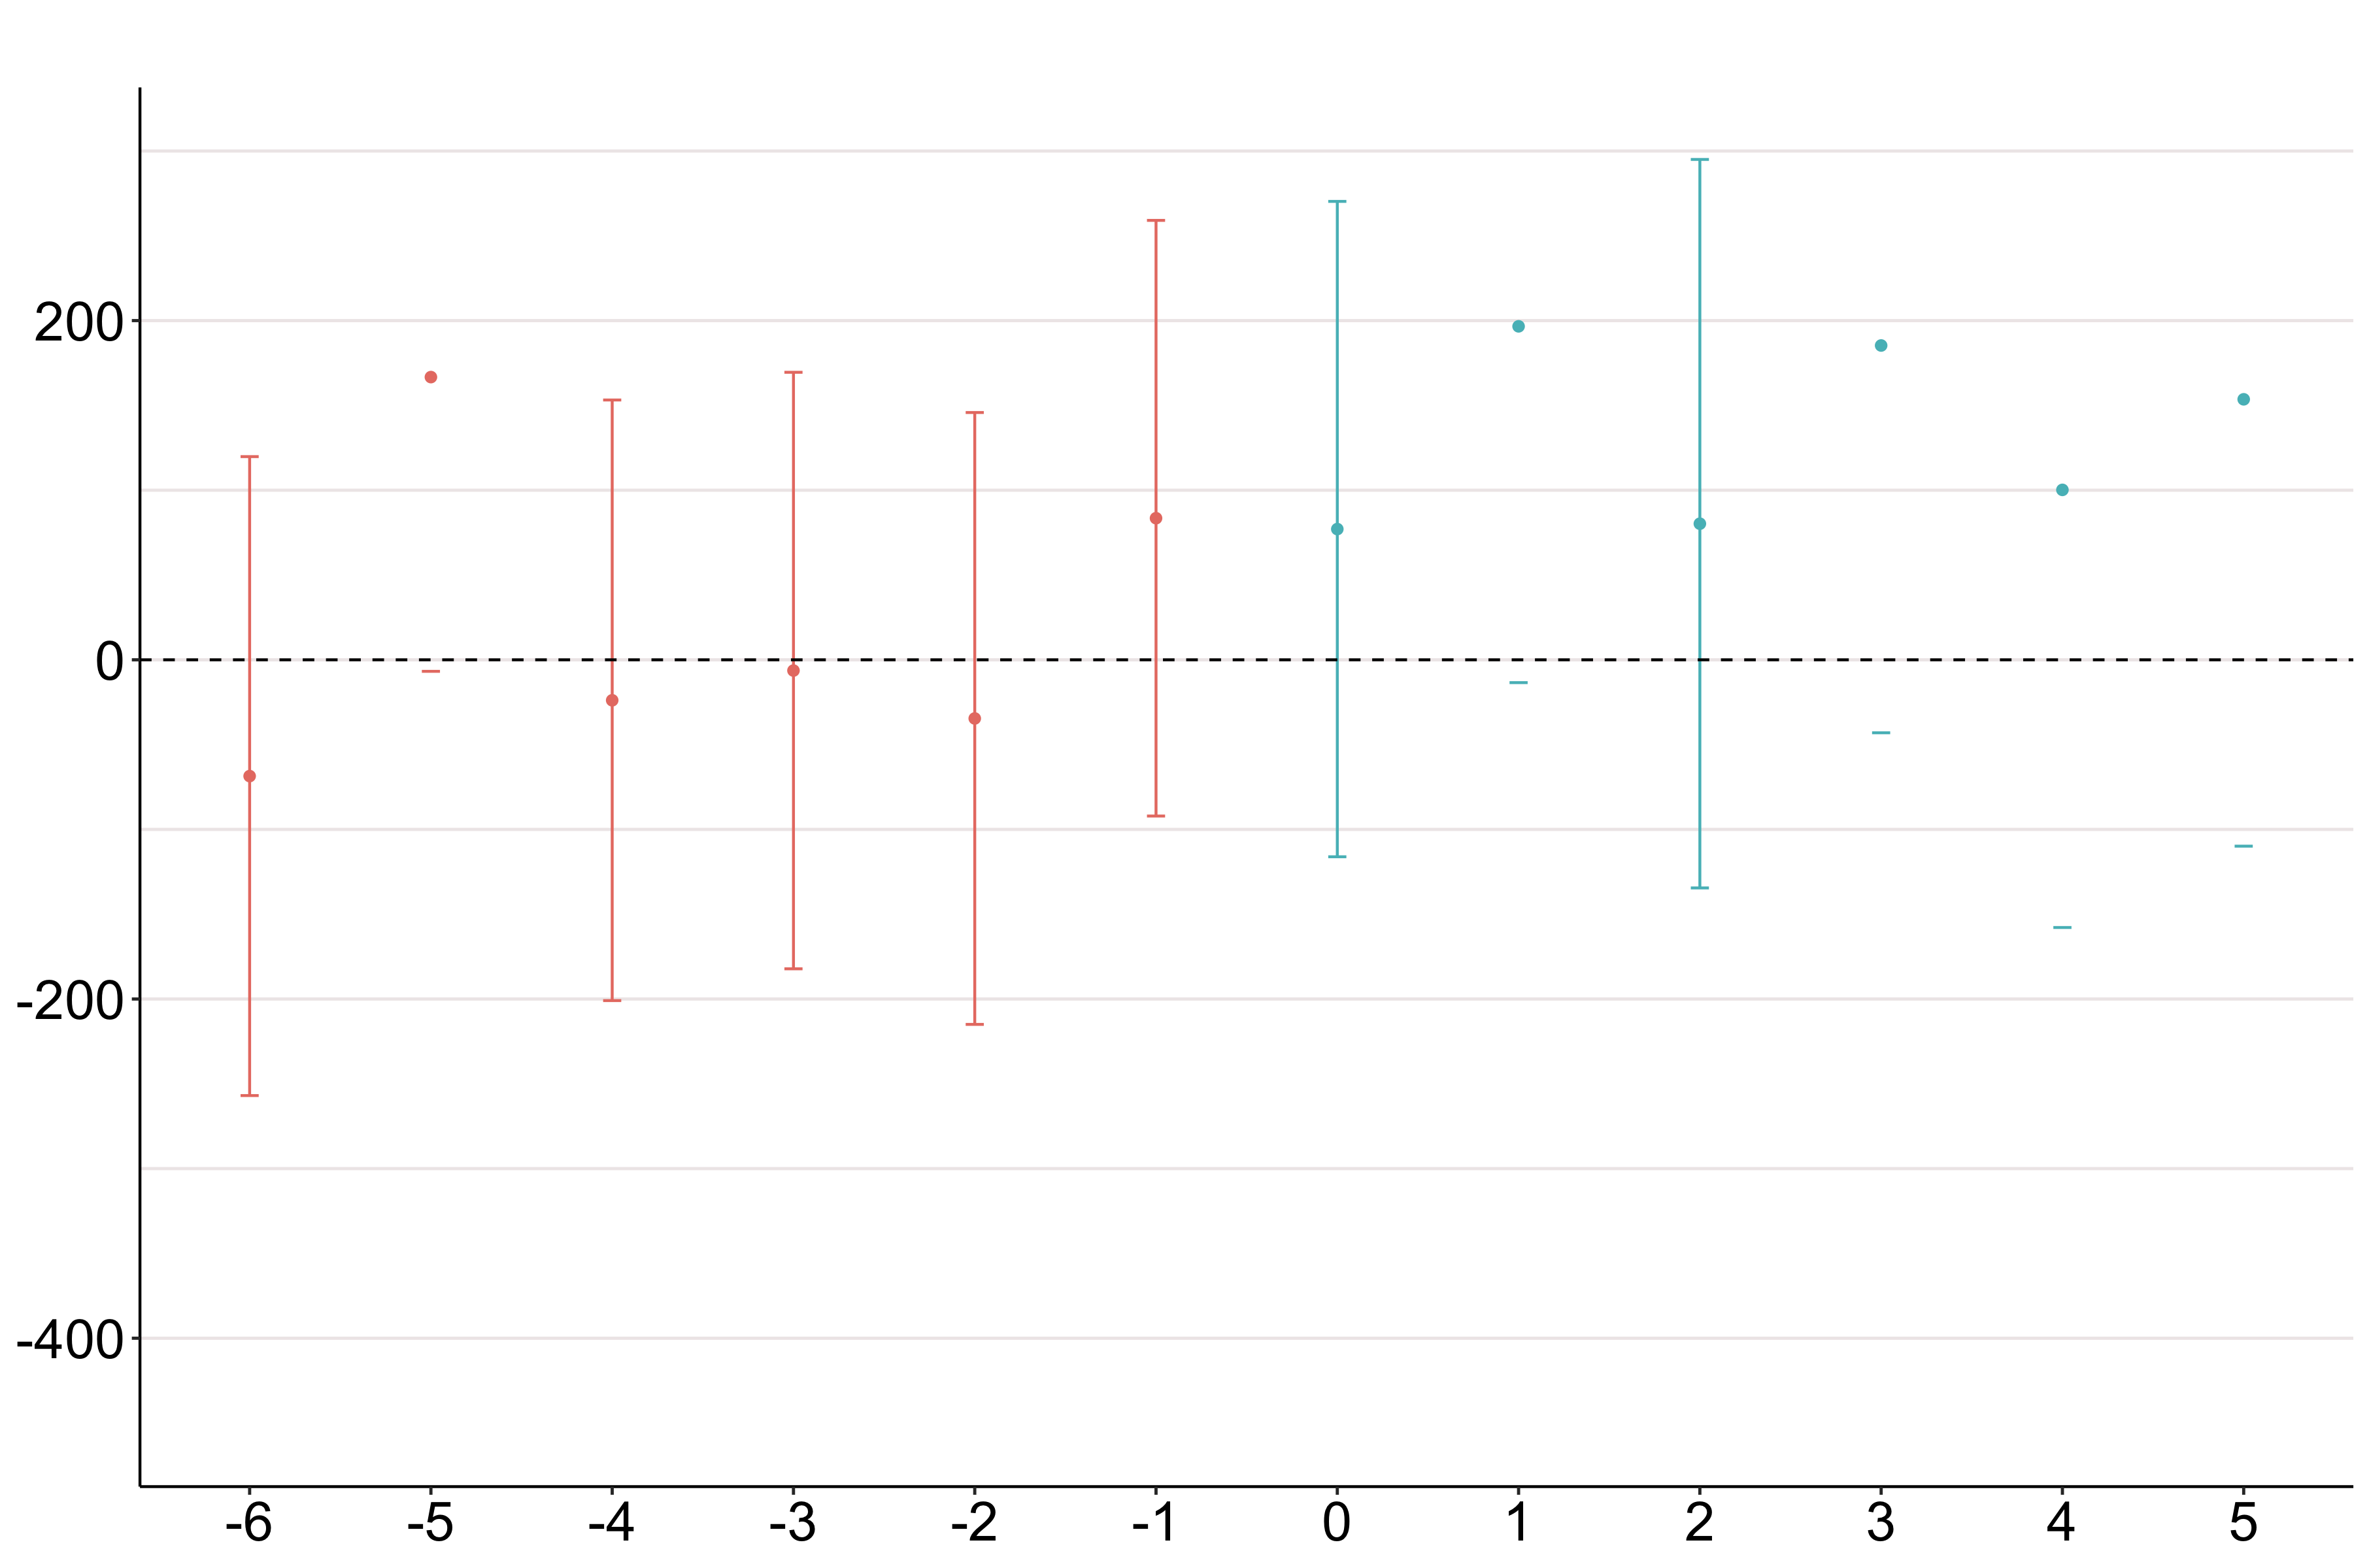
\includegraphics[width=.32\textwidth]{\figdir/netflows_antic5_es.png}
    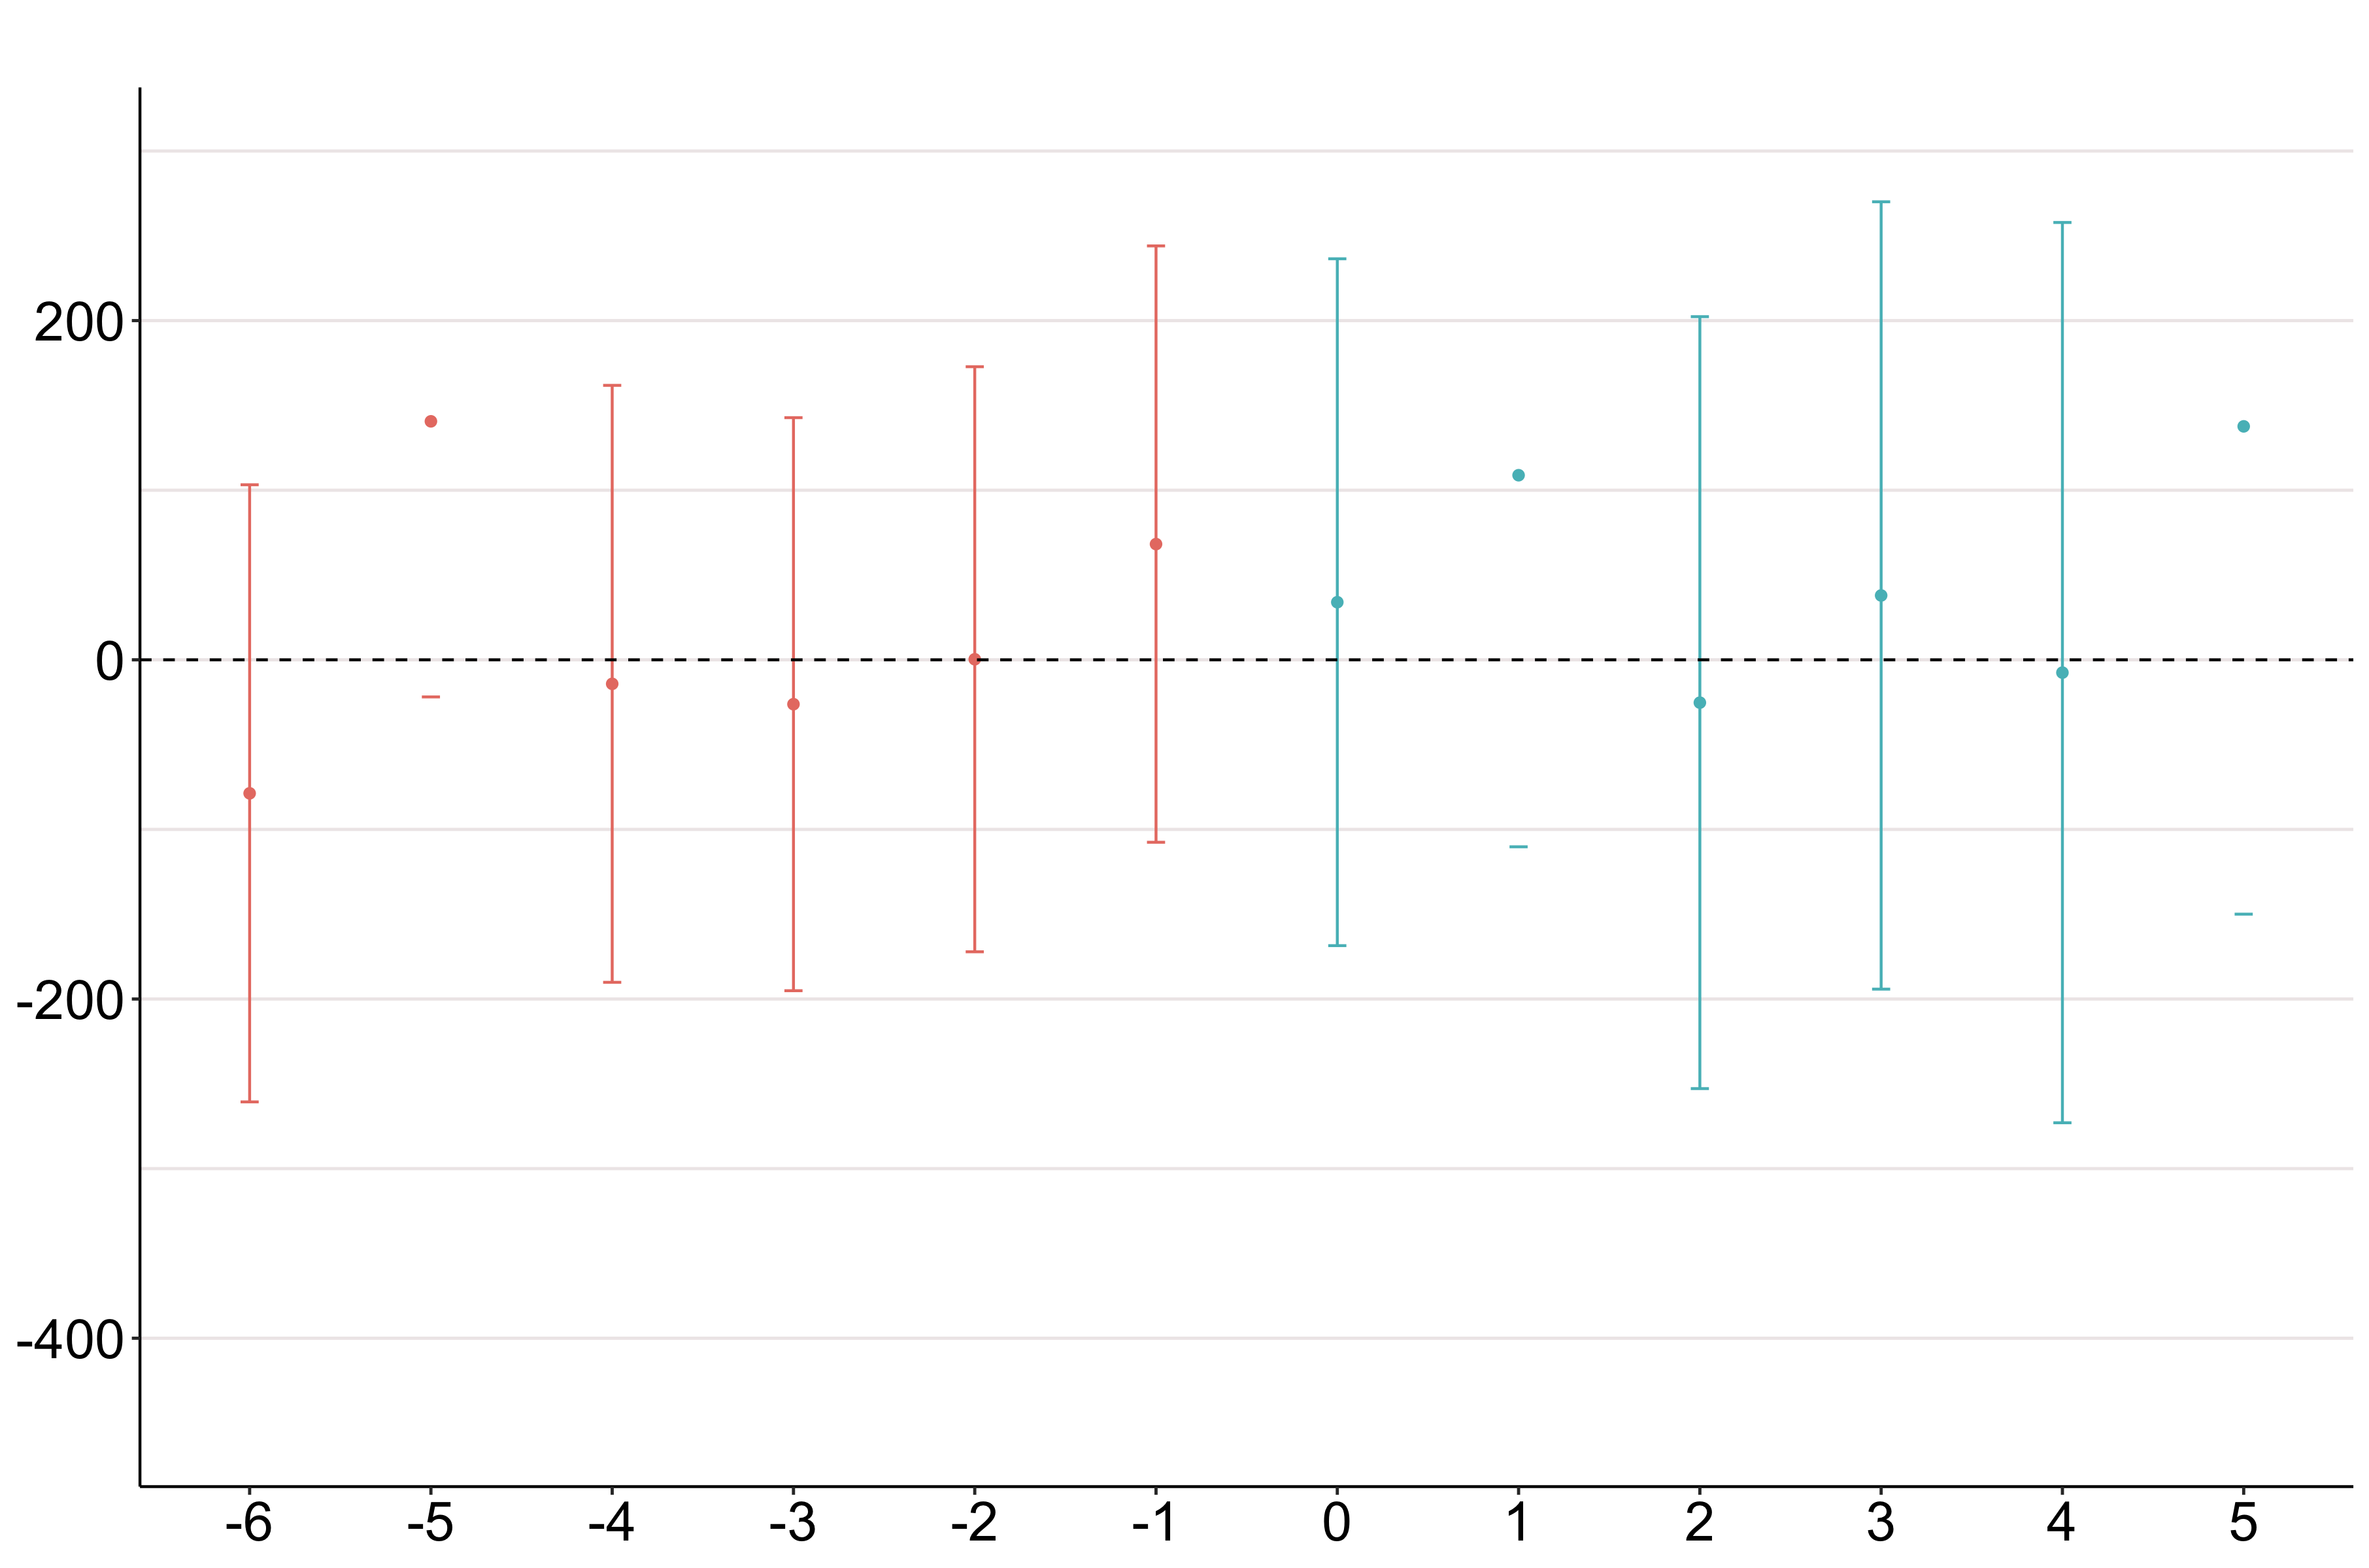
\includegraphics[width=.32\textwidth]{\figdir/netflows_antic6_es.png}
    \fignote{\textwidth}{...}
\end{figure}

\subsection{Unbalanced aggregation}%
\label{sub:unbalanced_aggregation}

The baseline specification relies on a panel balanced in event time and
thus only includes groups that have been exposed to treatment for at least 5
periods. Figure~\ref{fig:ub_comp} reproduces the baseline results in the left
panel and compares it with results based on the full sample.

As discussed in \citet{callaway2021difference} (section 3.1.1), these two
approaches entail a trade-off. When using the full sample, the aggregated
parameters are a function of the weighted average treatment effects for each
group $e$ periods after treatment (which is what we want) as well as
compositional changes due to different groups being included for different
periods $e$ and different weights attached to these groups. While parameters
aggregated using a panel balanced in event time do not suffer from
compositional and weighting changes, but are calculated based on a smaller
number of groups.

As expected, using the full data reduces the size of the confidence intervals.
But the results are otherwise very similar.

\begin{figure}[H]
    \centering
    \caption{Balanced and unbalanced aggregation}%
    \label{fig:ub_comp}
    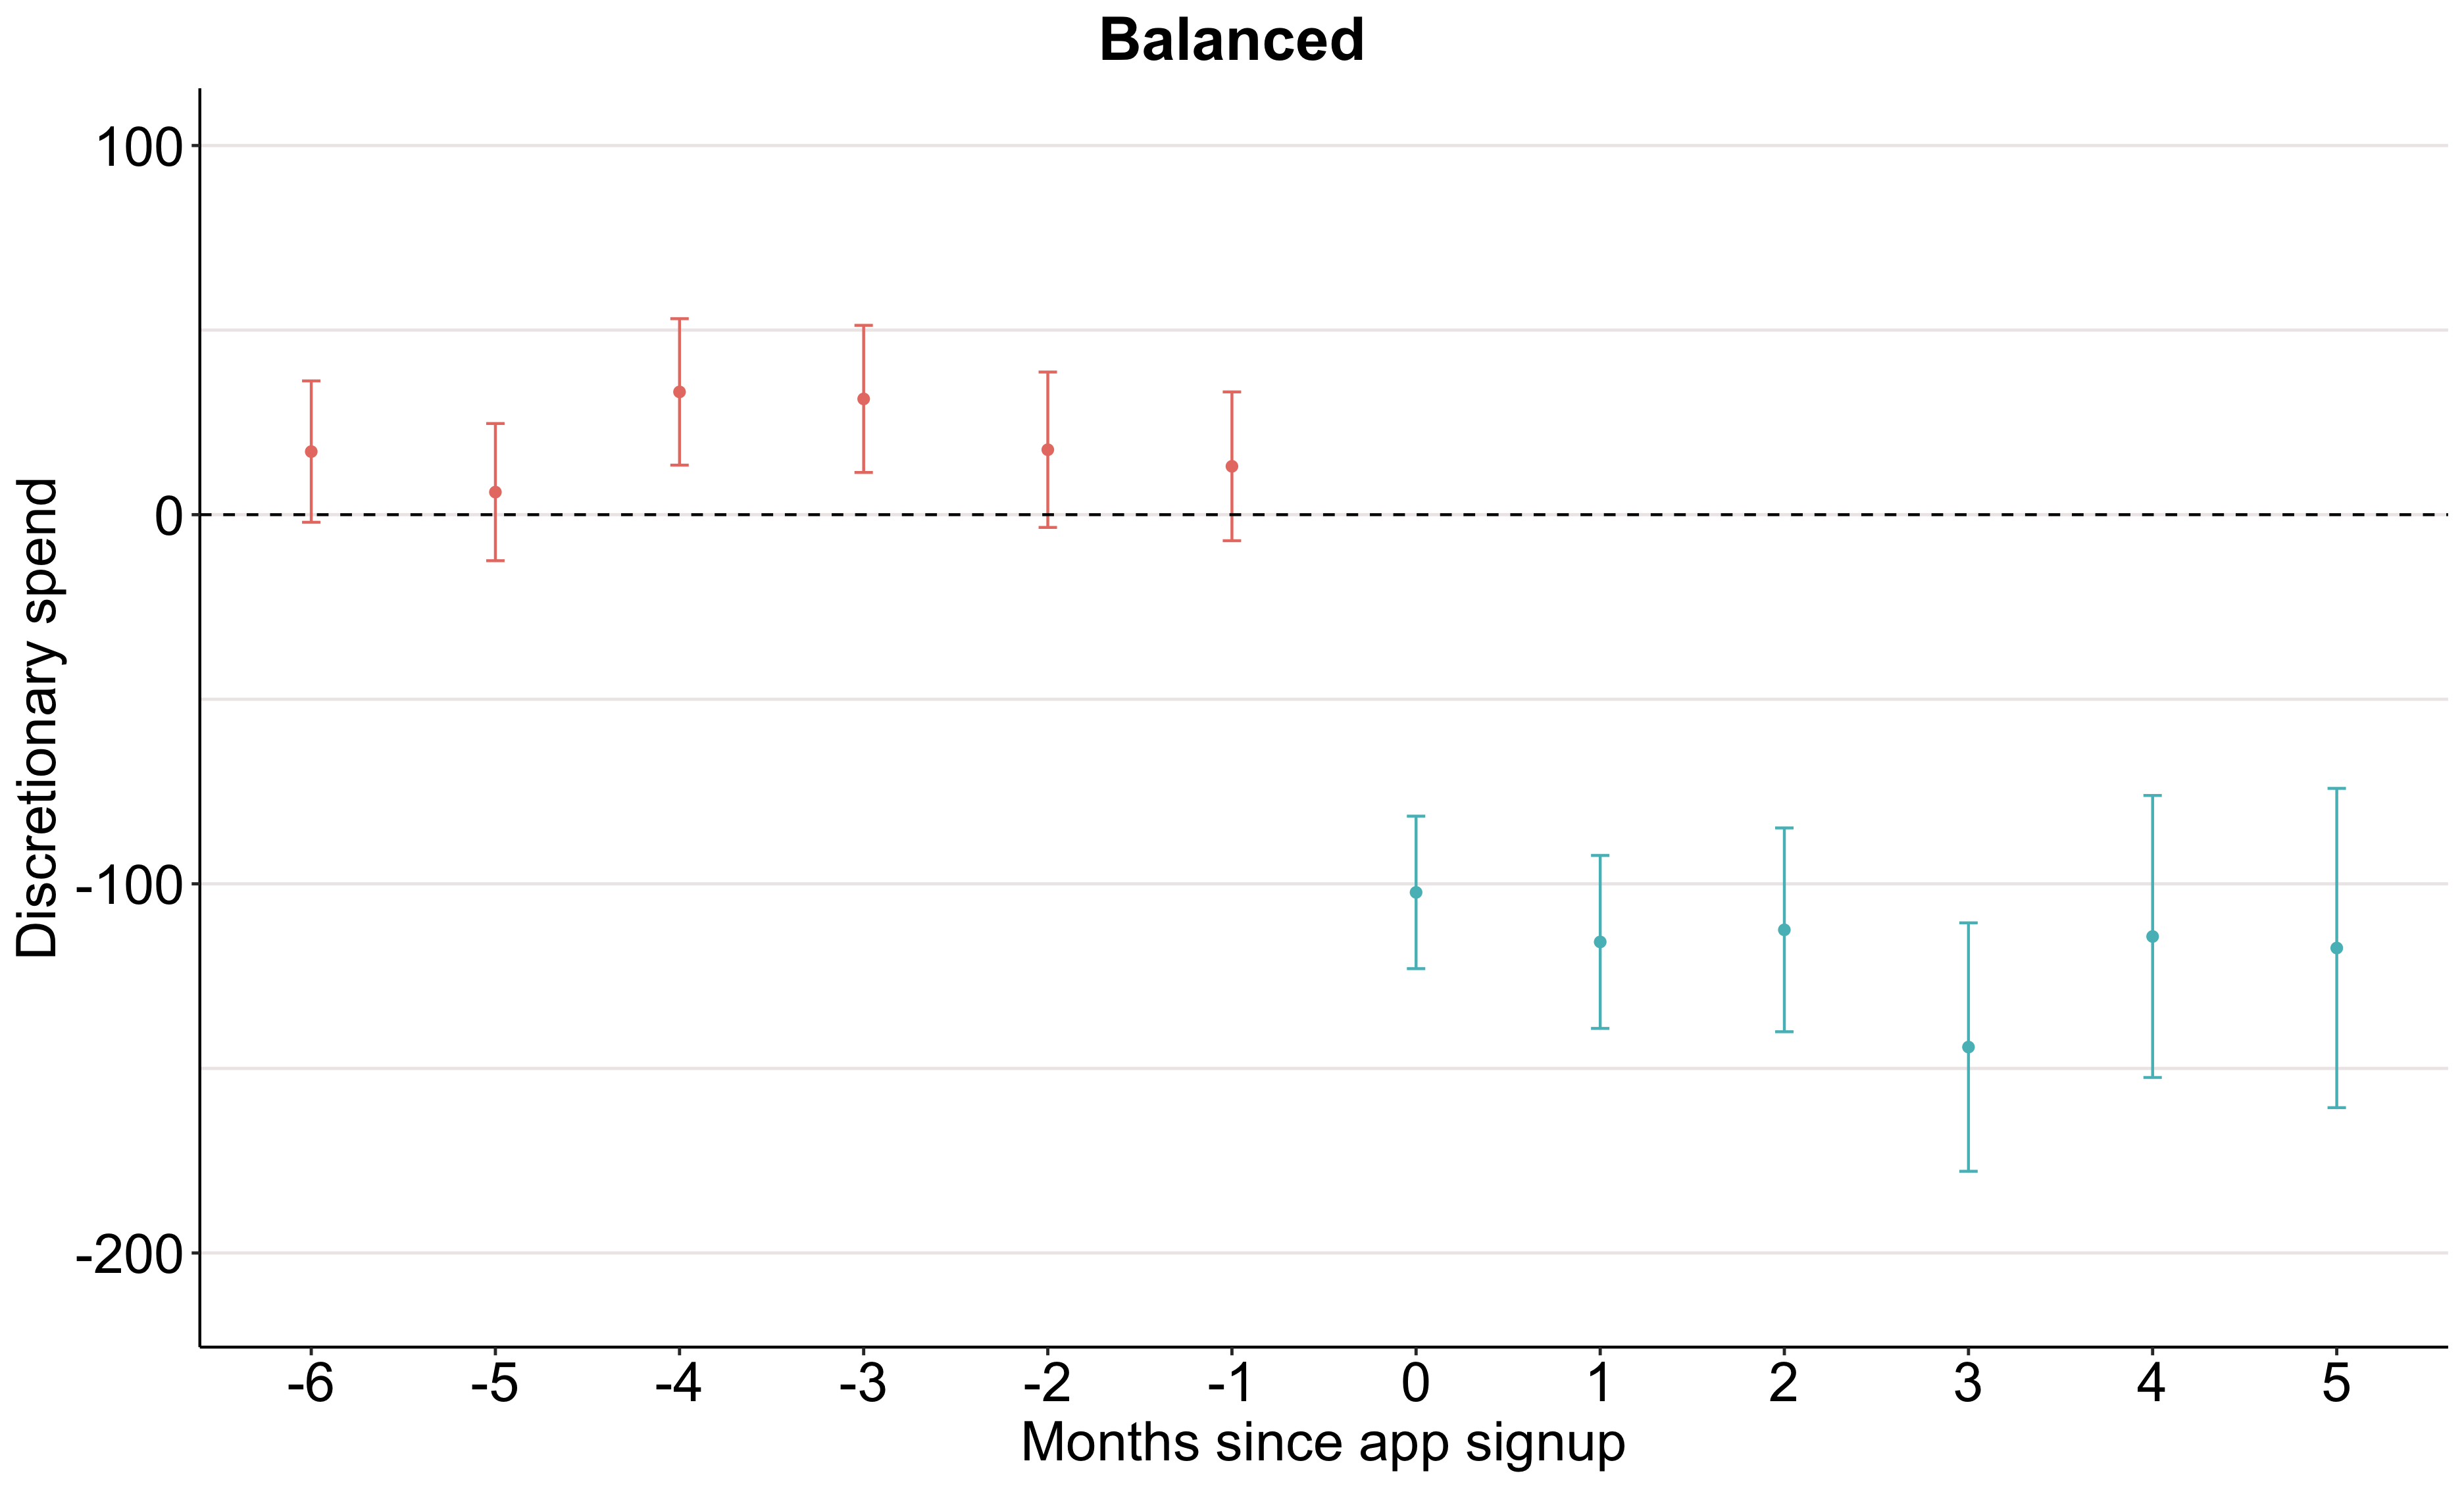
\includegraphics[width=.49\textwidth]{\figdir/dspend_cond_bal_es.png}
    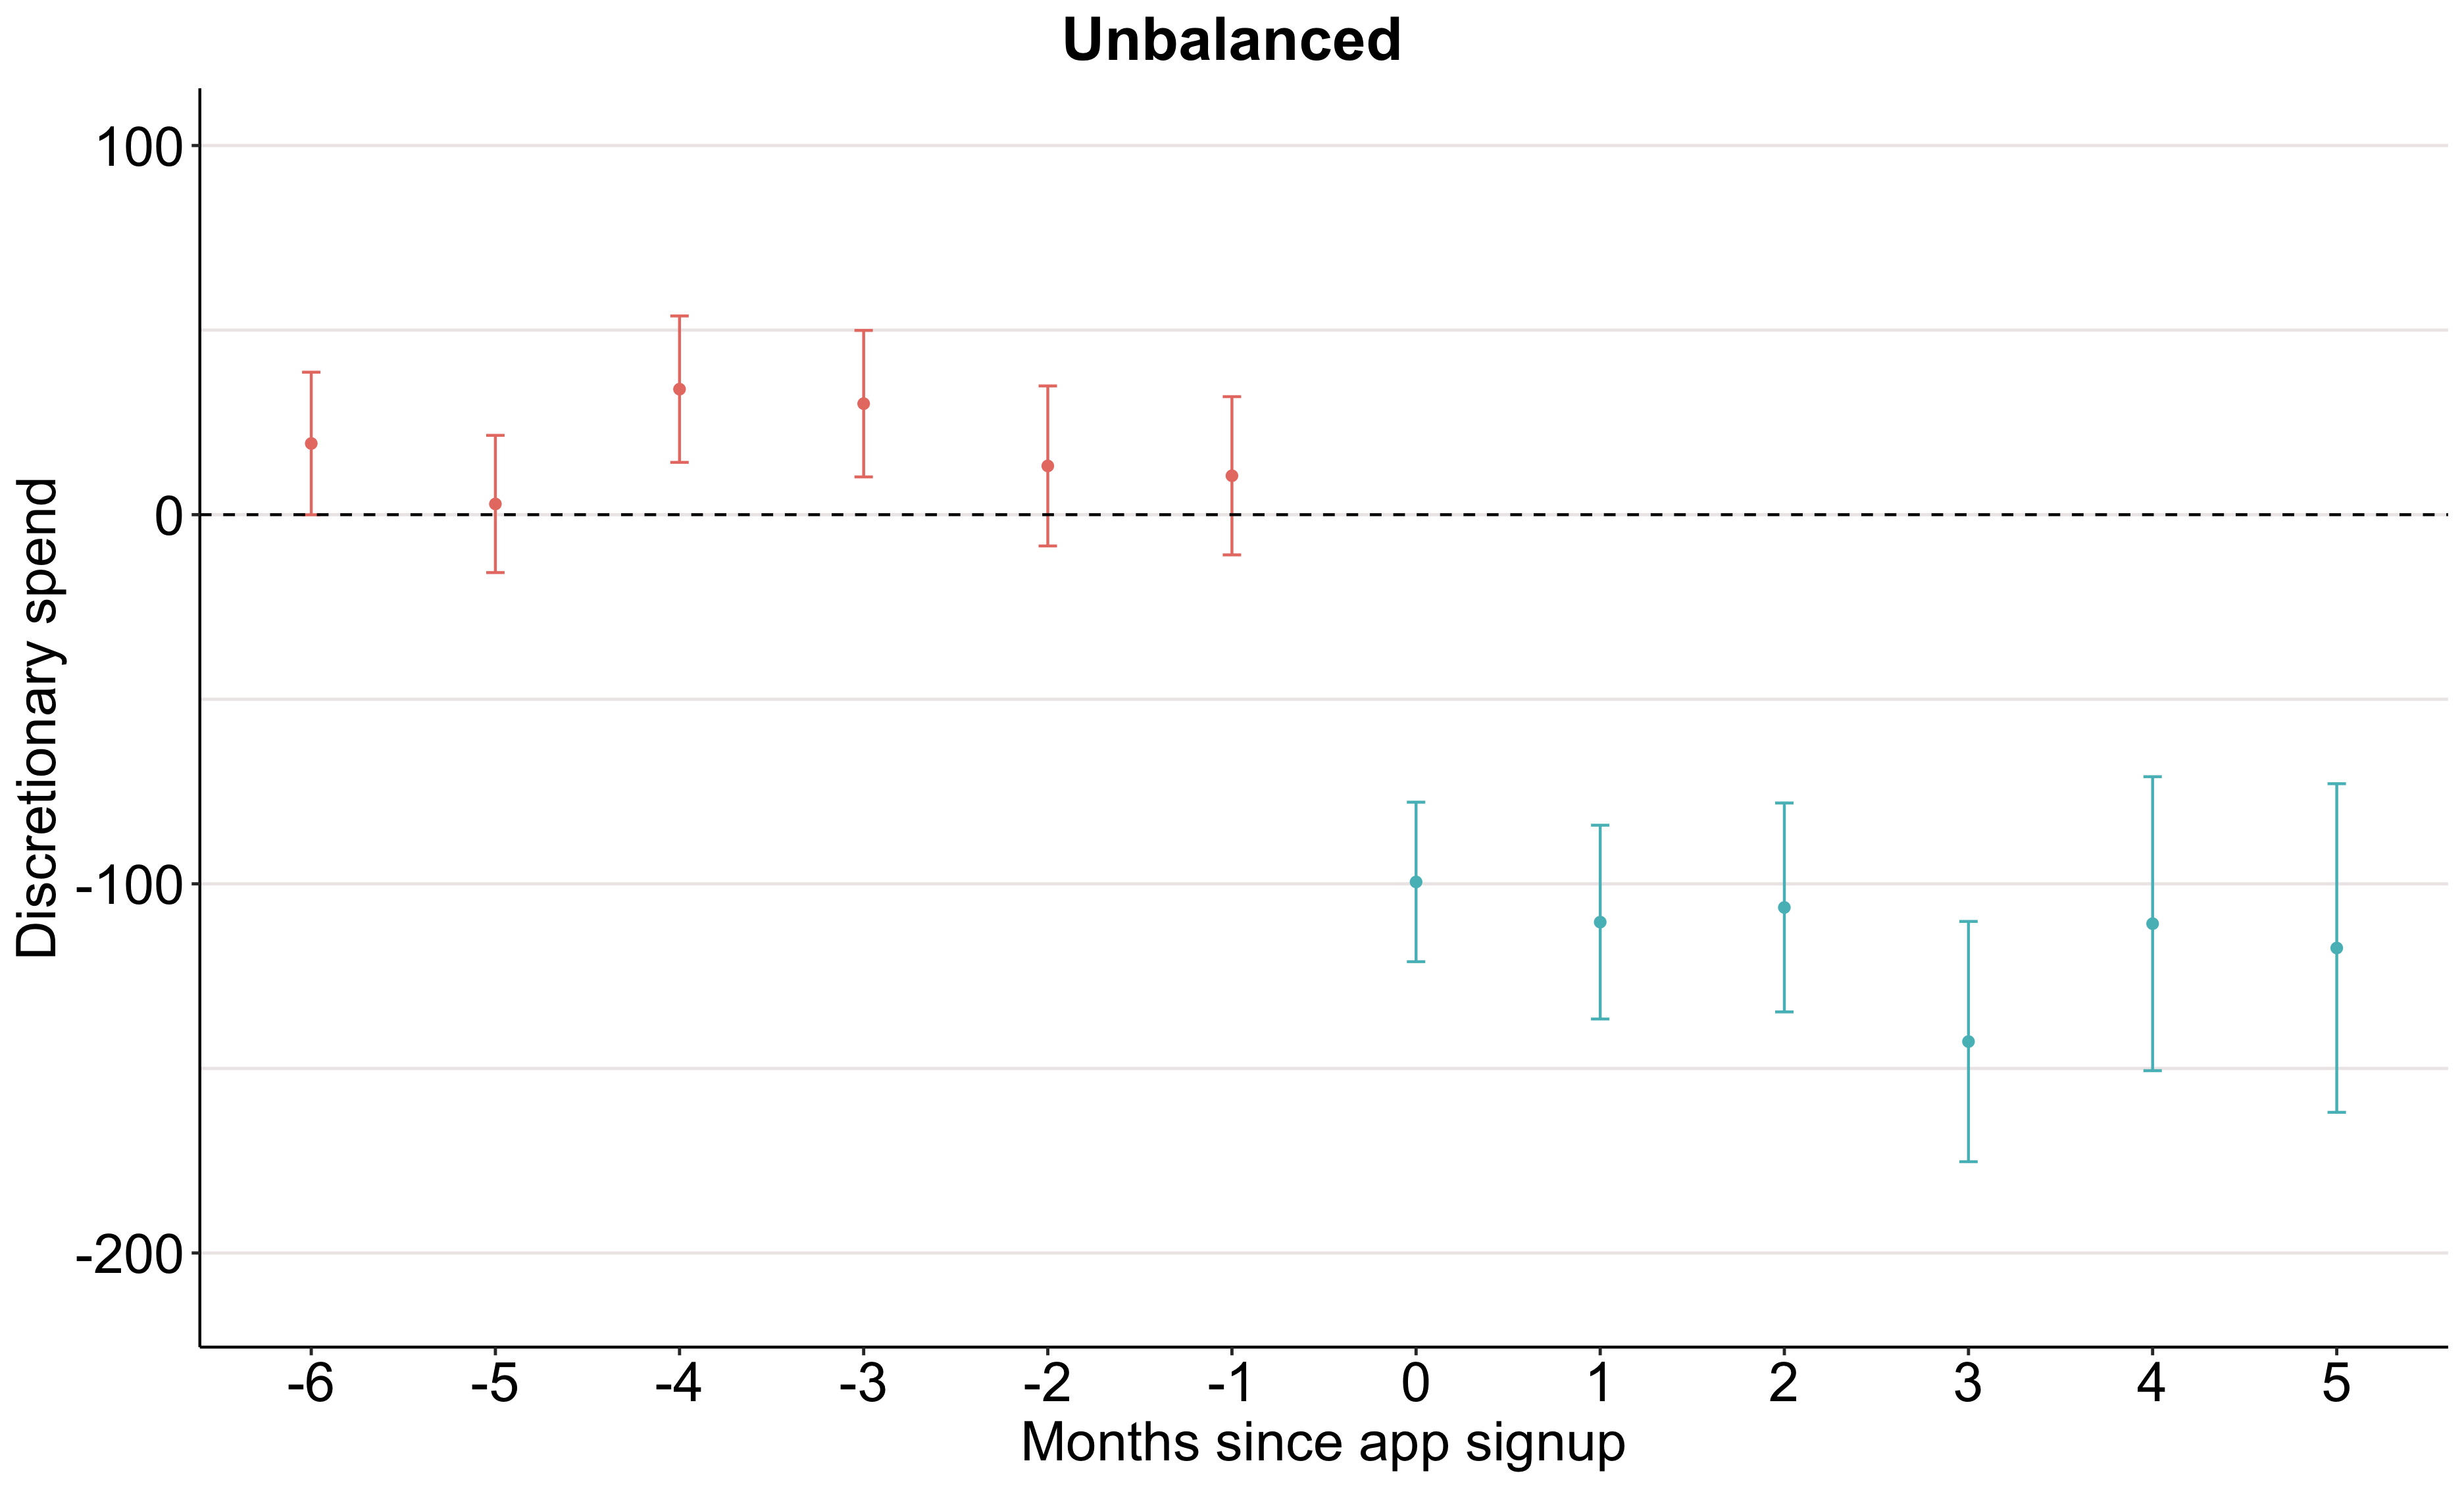
\includegraphics[width=.49\textwidth]{\figdir/dspend_cond_unbal_es.png}
    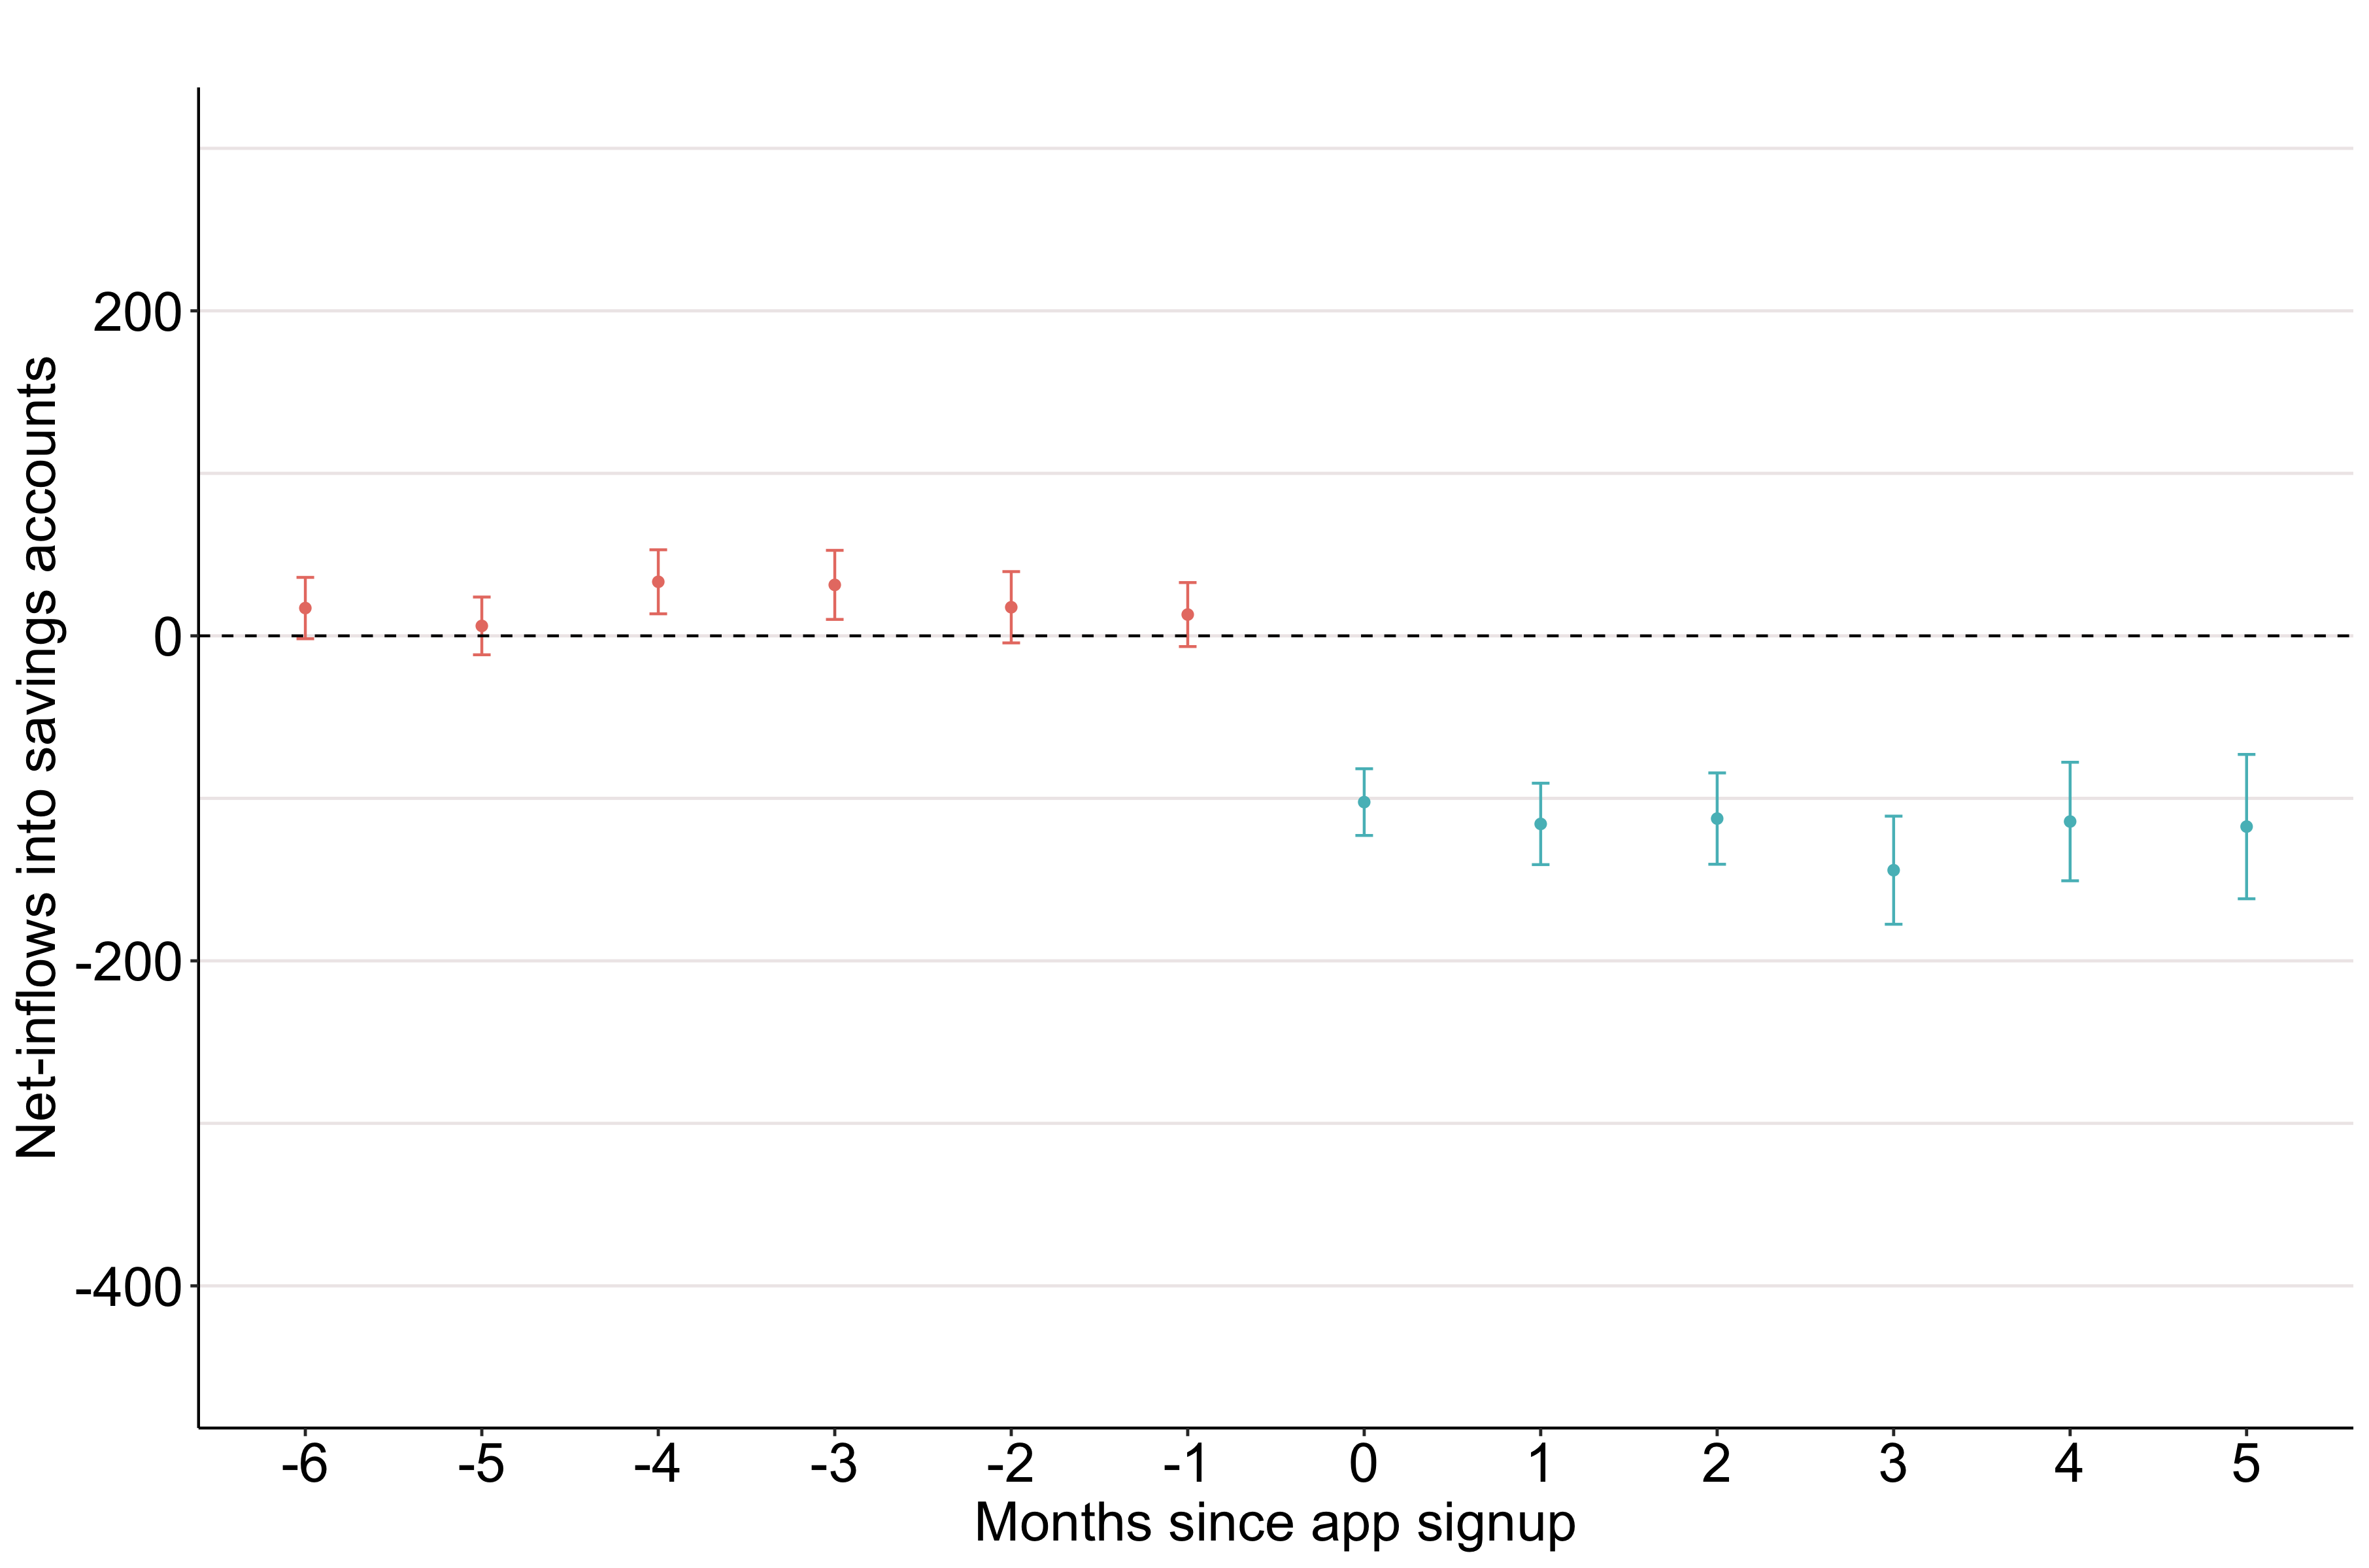
\includegraphics[width=.49\textwidth]{\figdir/netflows_cond_bal_es.png}
    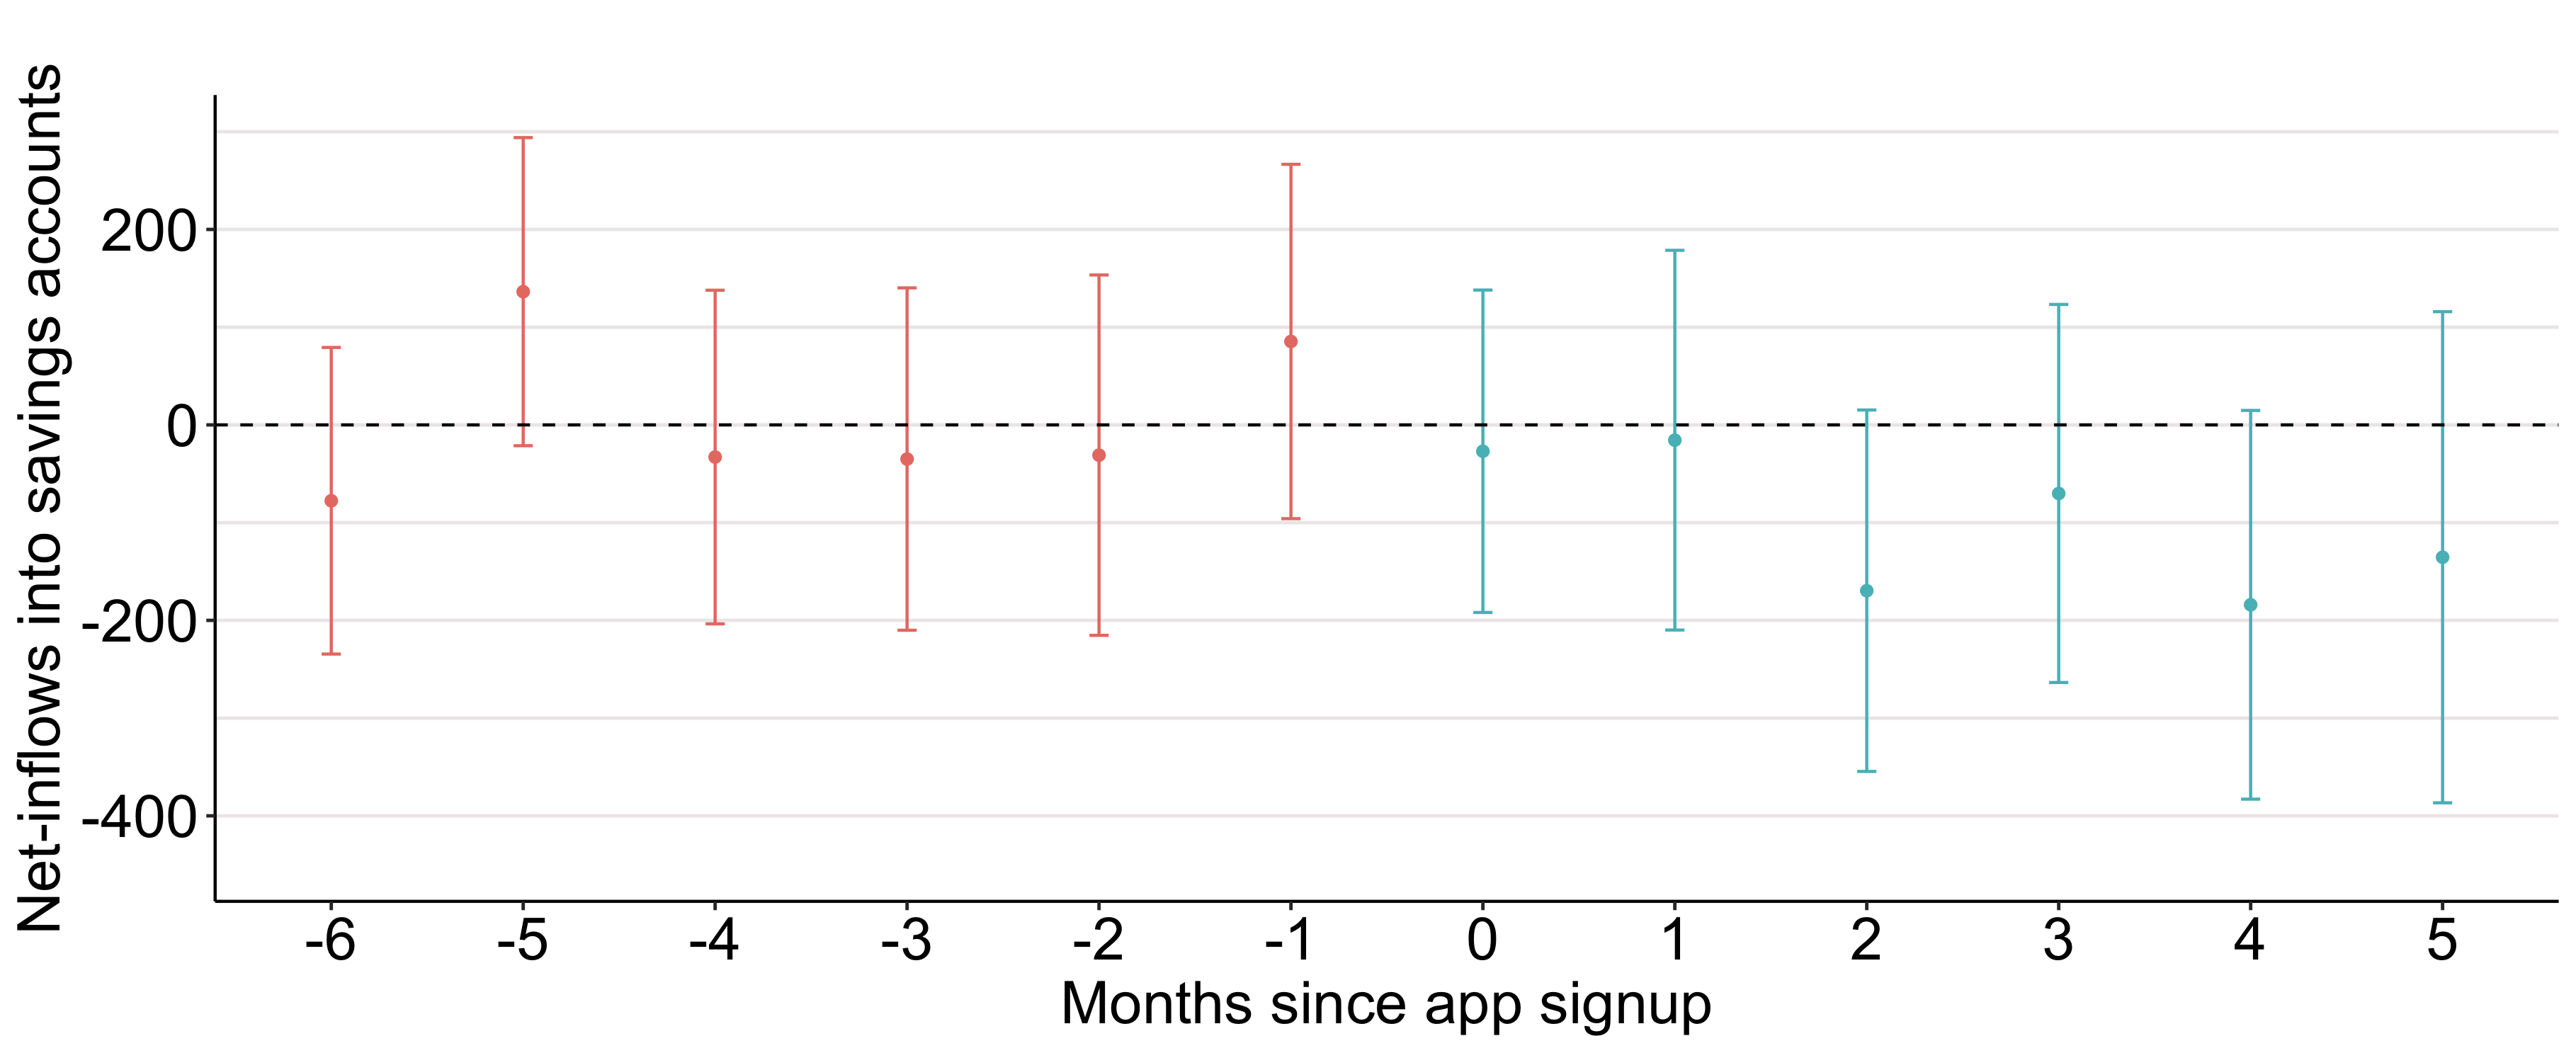
\includegraphics[width=.49\textwidth]{\figdir/netflows_cond_unbal_es.png}
    \fignote{\textwidth}{...}
\end{figure}



\subsection{Inflows and outflows}%
\label{sub:inflows_and_outflows}

\begin{itemize}
    \item Netflows are unchanged because effects on inflows and outflows closely mirror
        each other.
\end{itemize}

\begin{figure}[H]
    \centering
    \caption{Inflows and outflows}%
    \label{fig:in_out_results}
    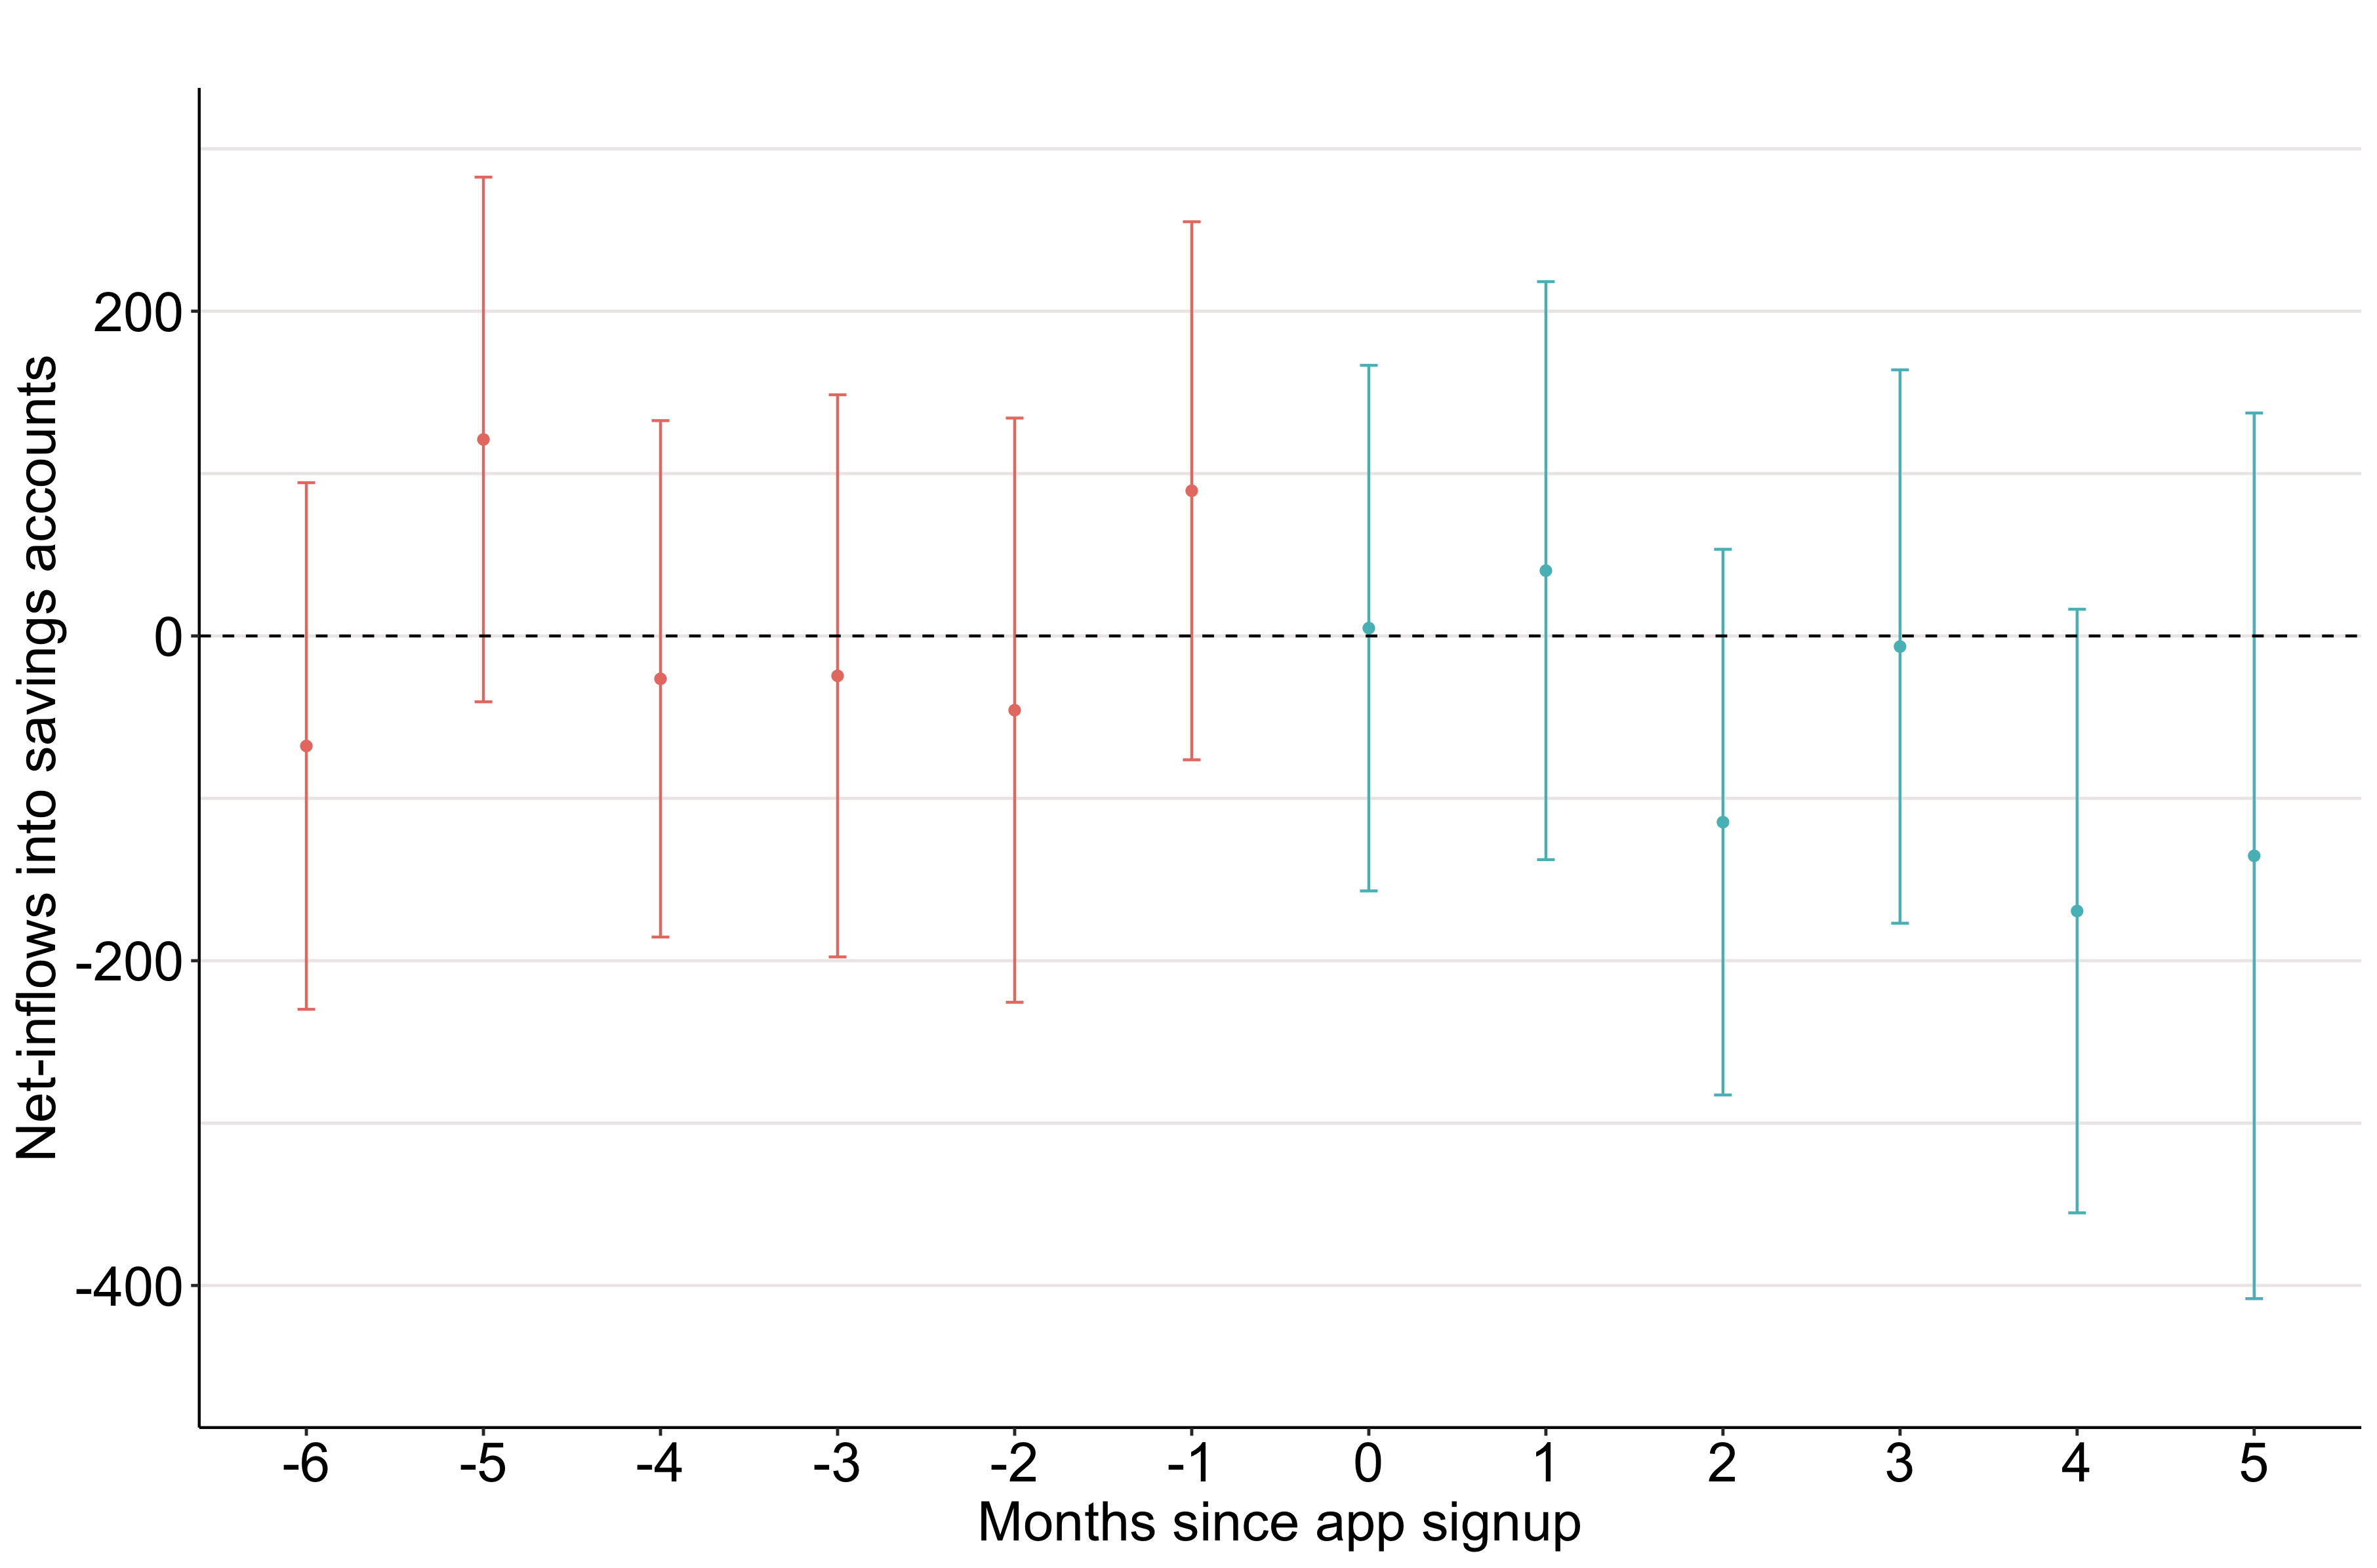
\includegraphics[width=.32\textwidth]{\figdir/netflows_cond_es.png}
    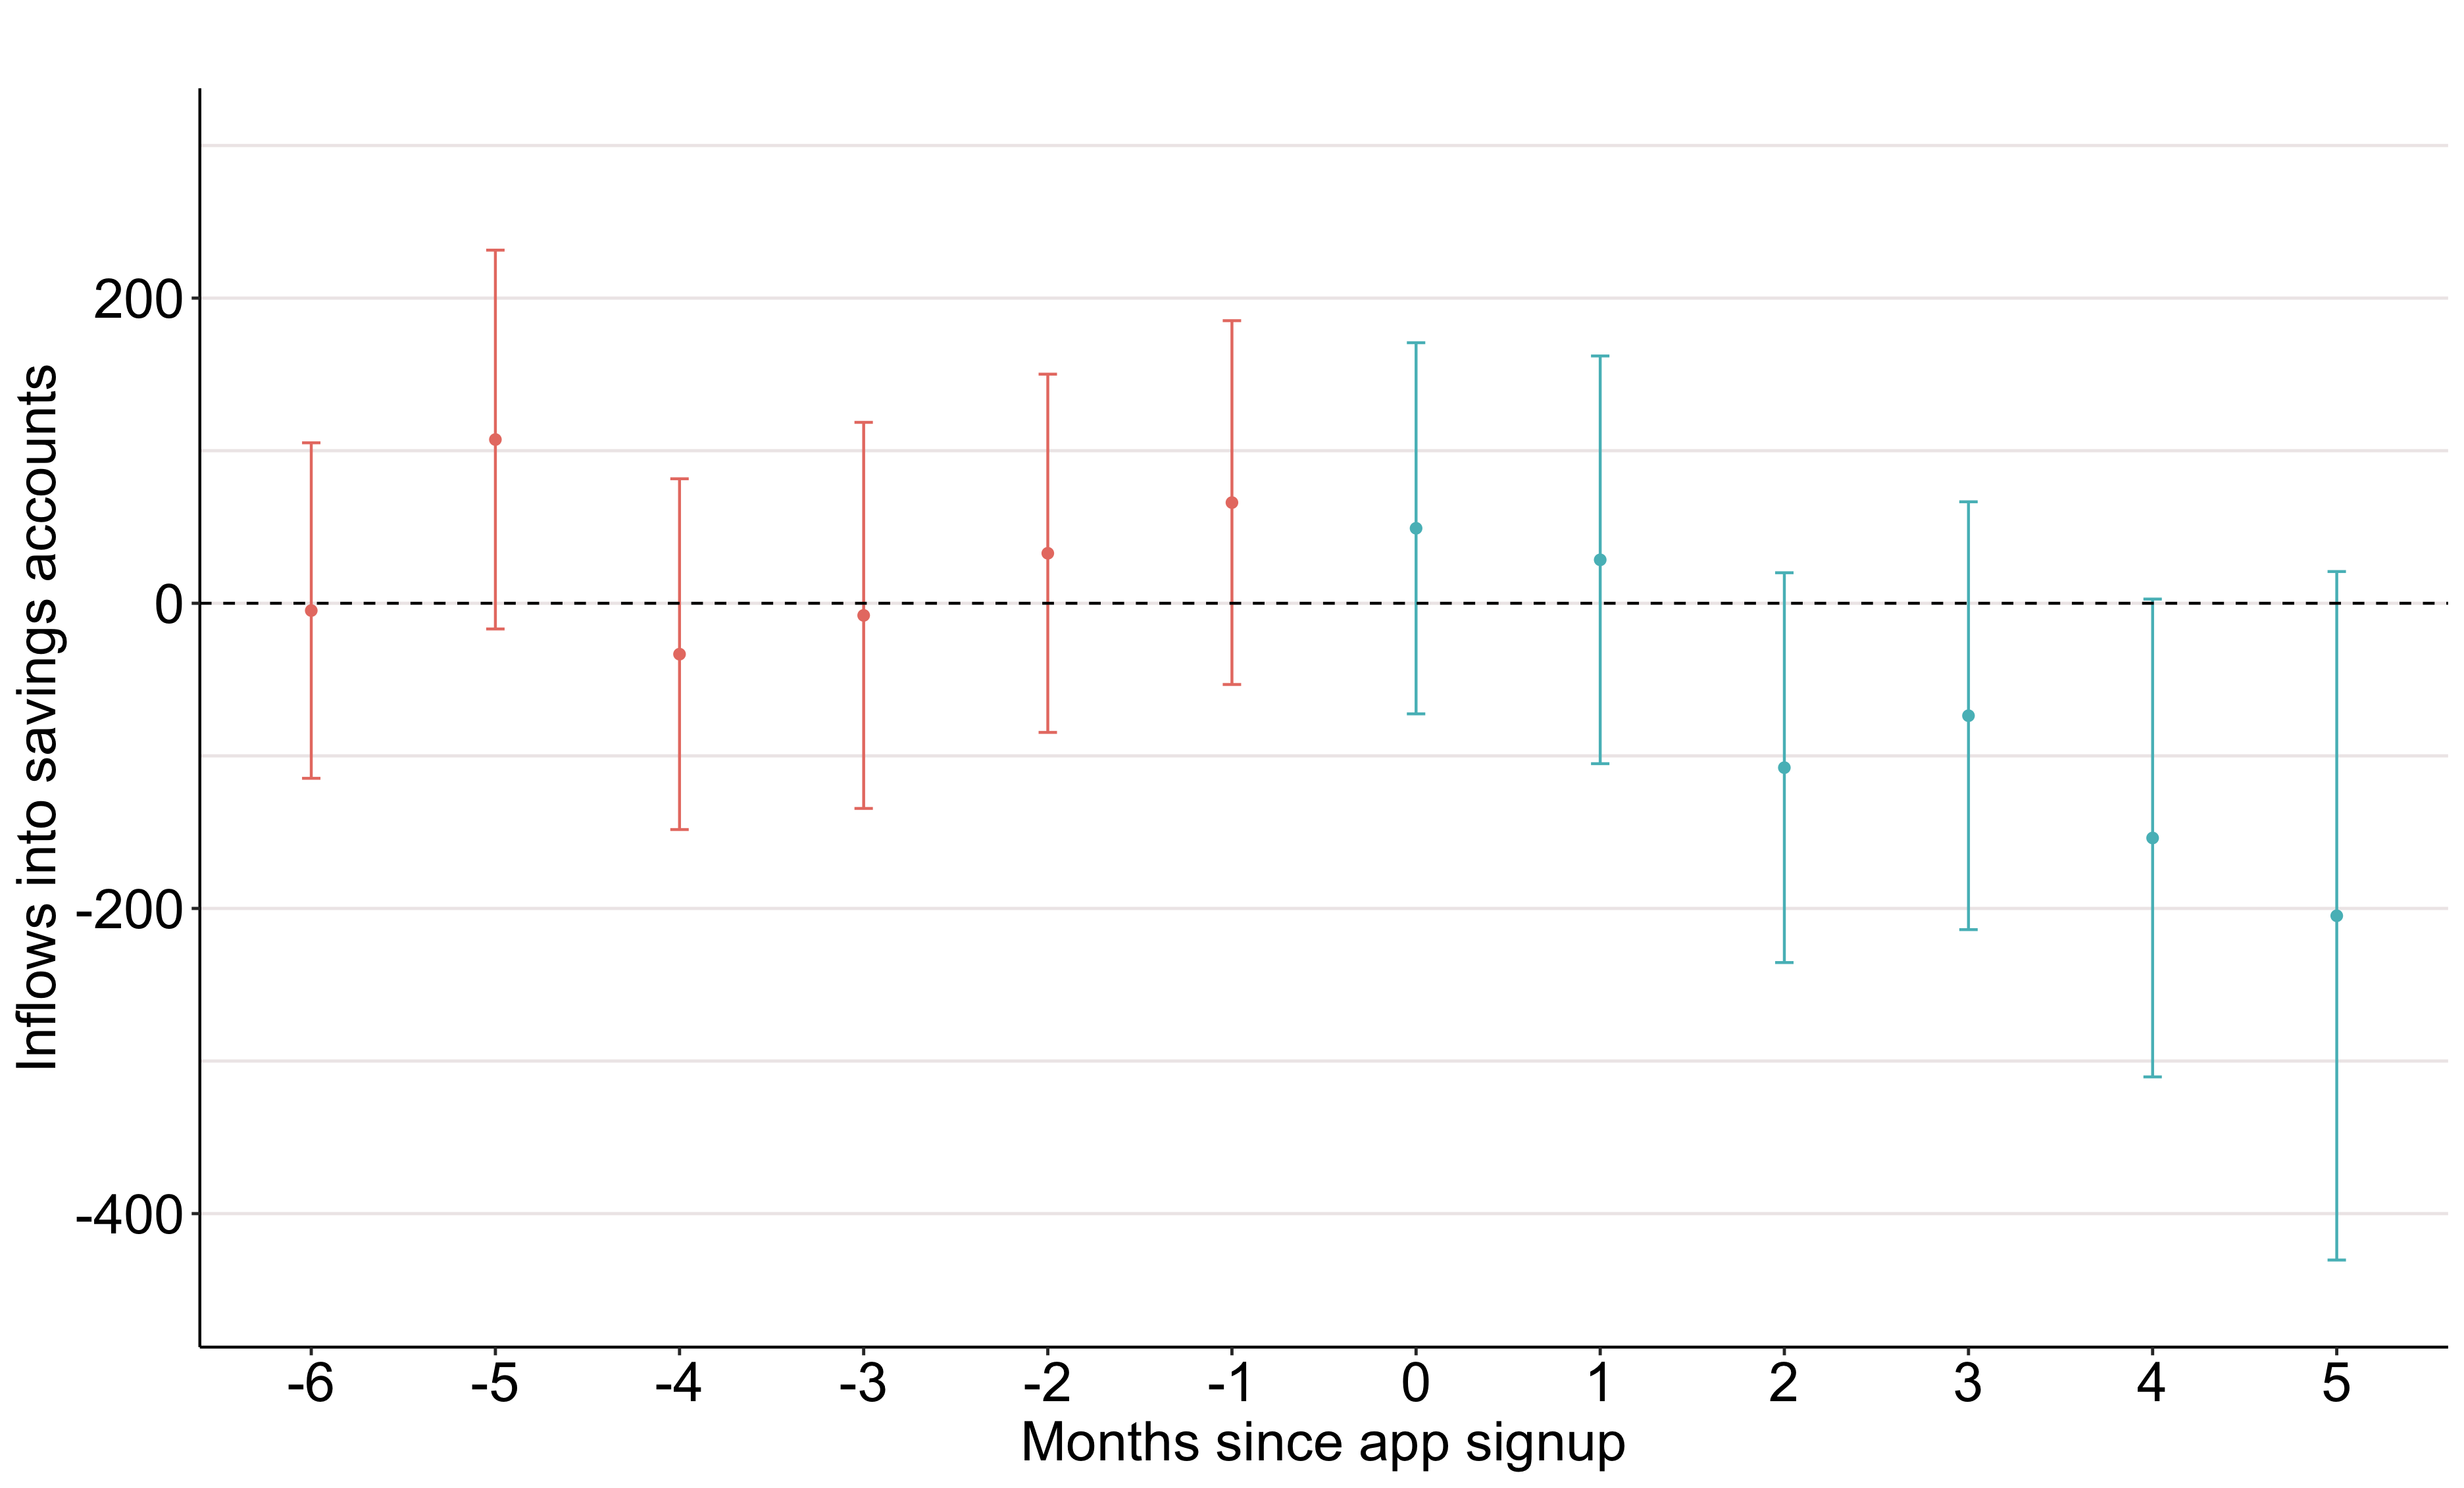
\includegraphics[width=.32\textwidth]{\figdir/inflows_cond_es.png}
    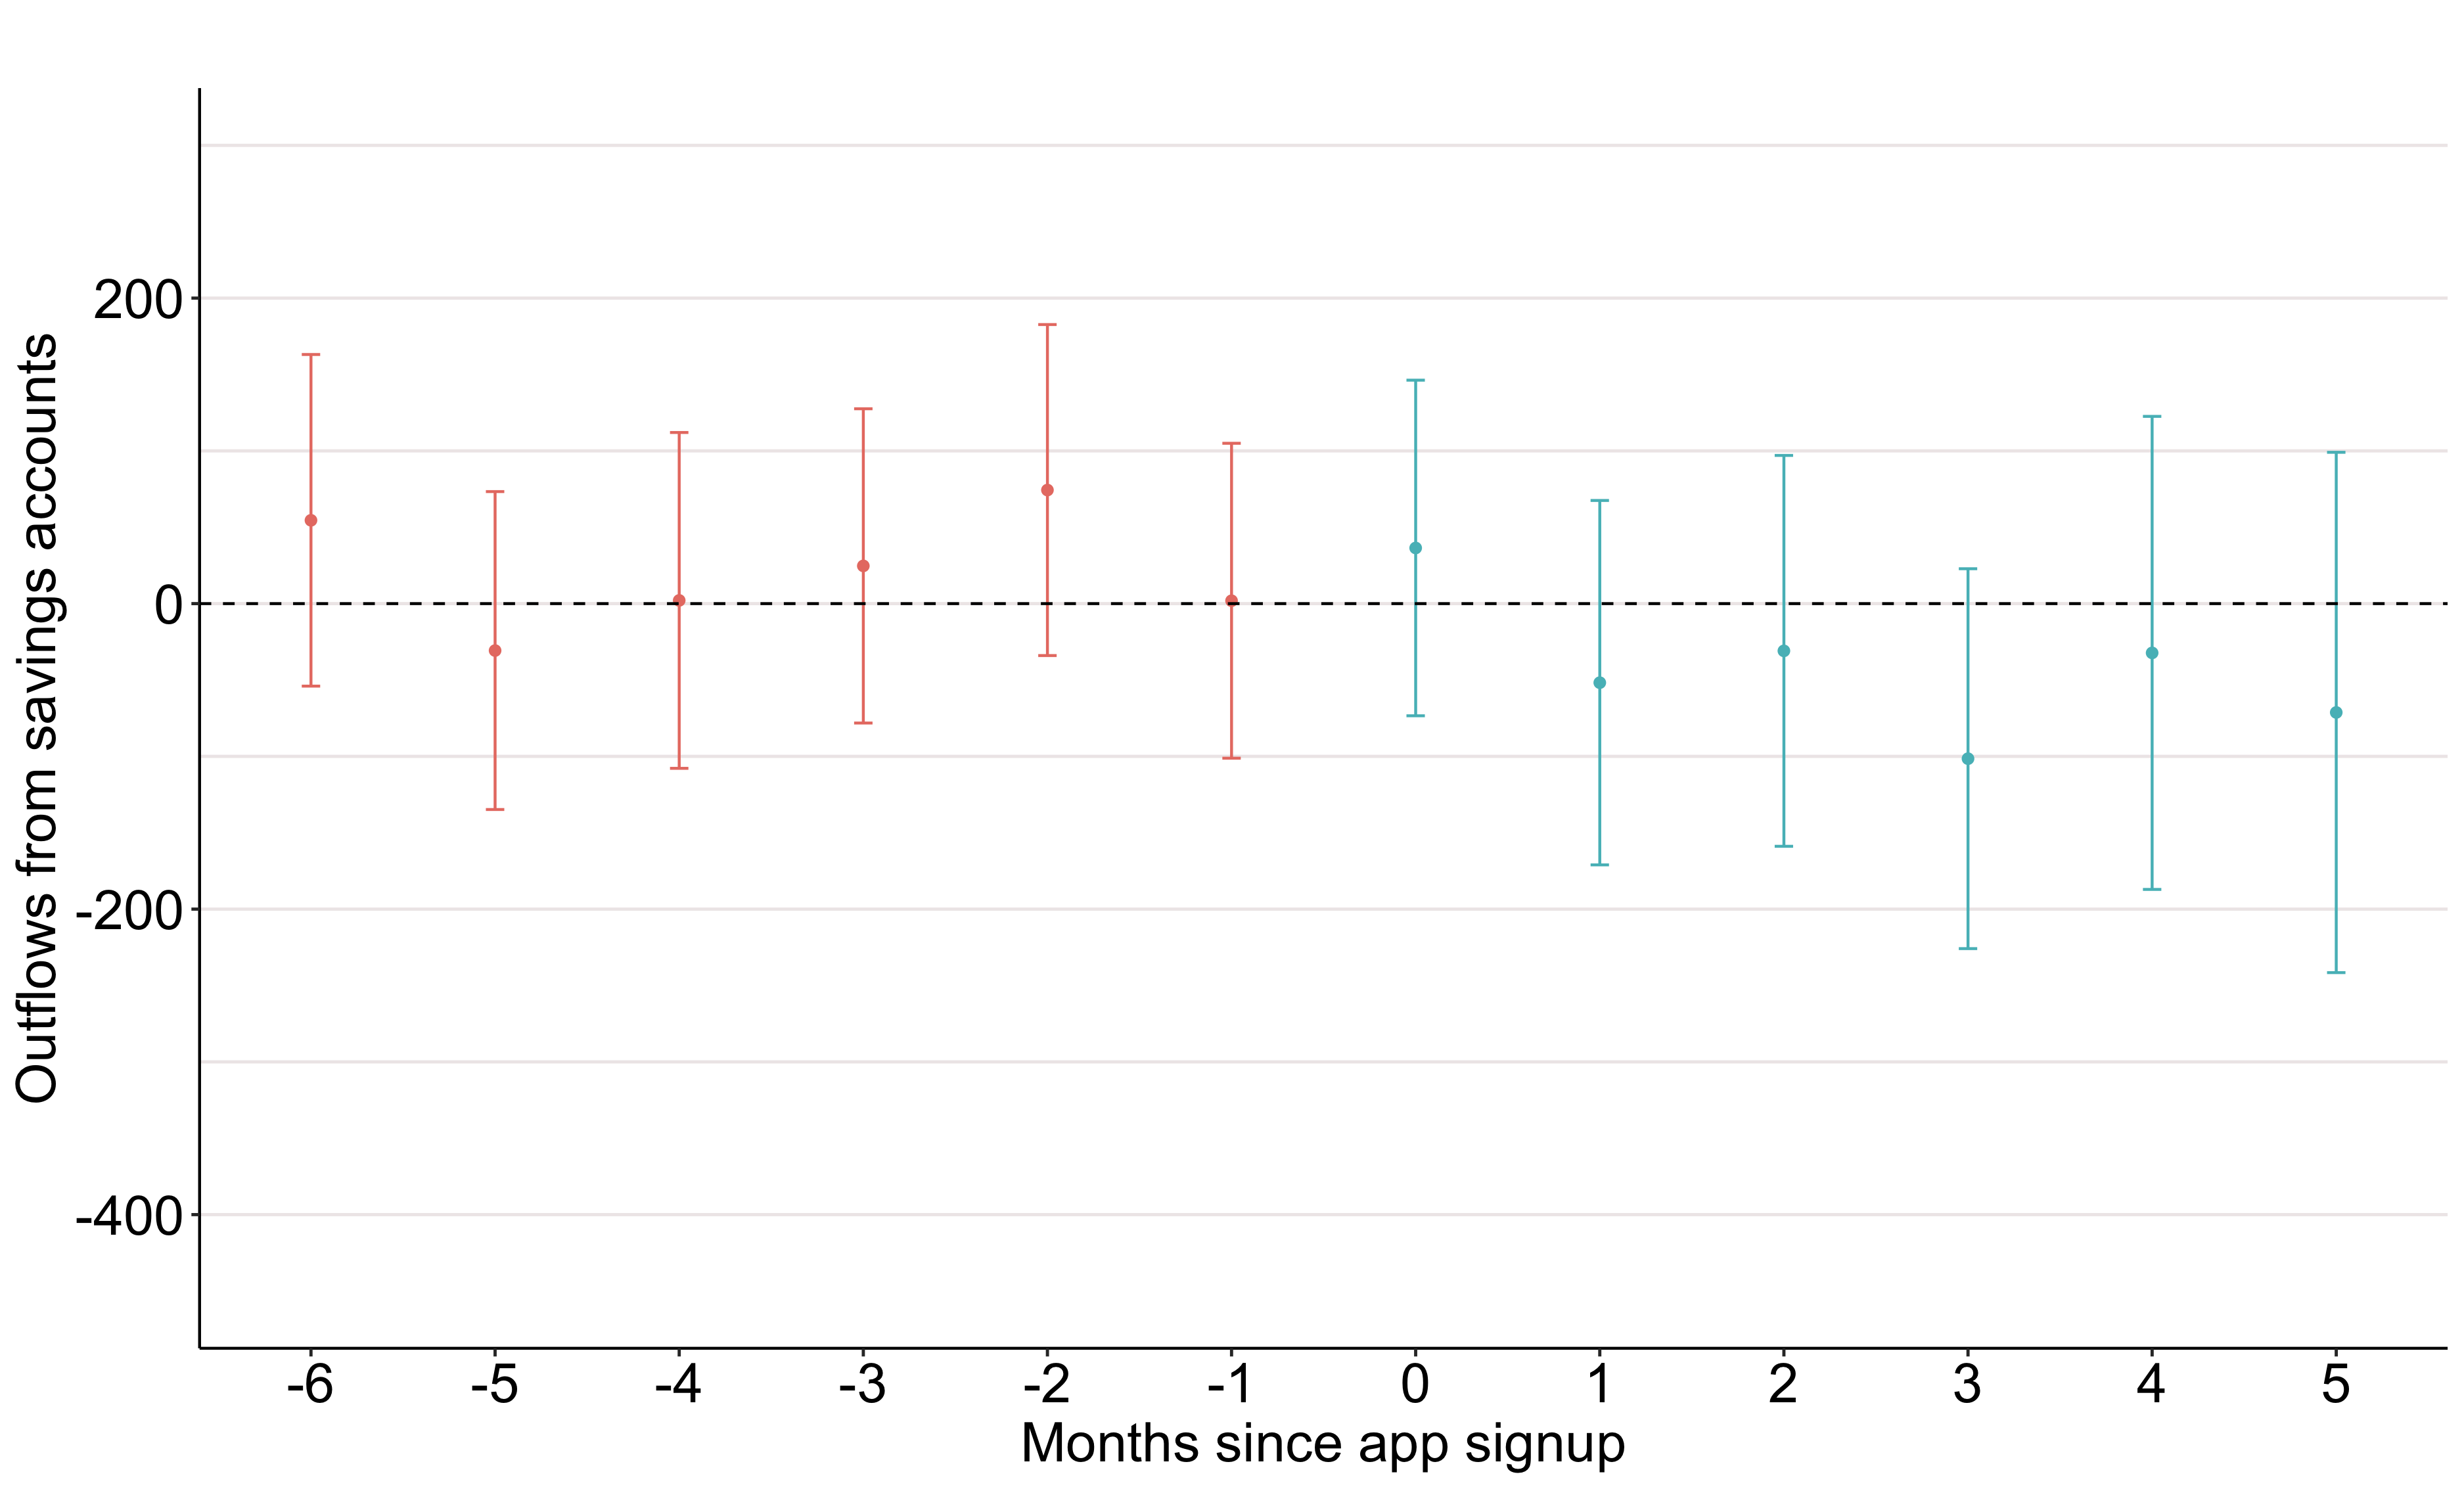
\includegraphics[width=.32\textwidth]{\figdir/outflows_cond_es.png}
    \fignote{\textwidth}{...}
\end{figure}


% \subsection{Robustness}%
% \label{sub:robustness}

% \begin{figure}[H]
%     \centering
%     \caption{New results}%
%     \label{fig:new}
%     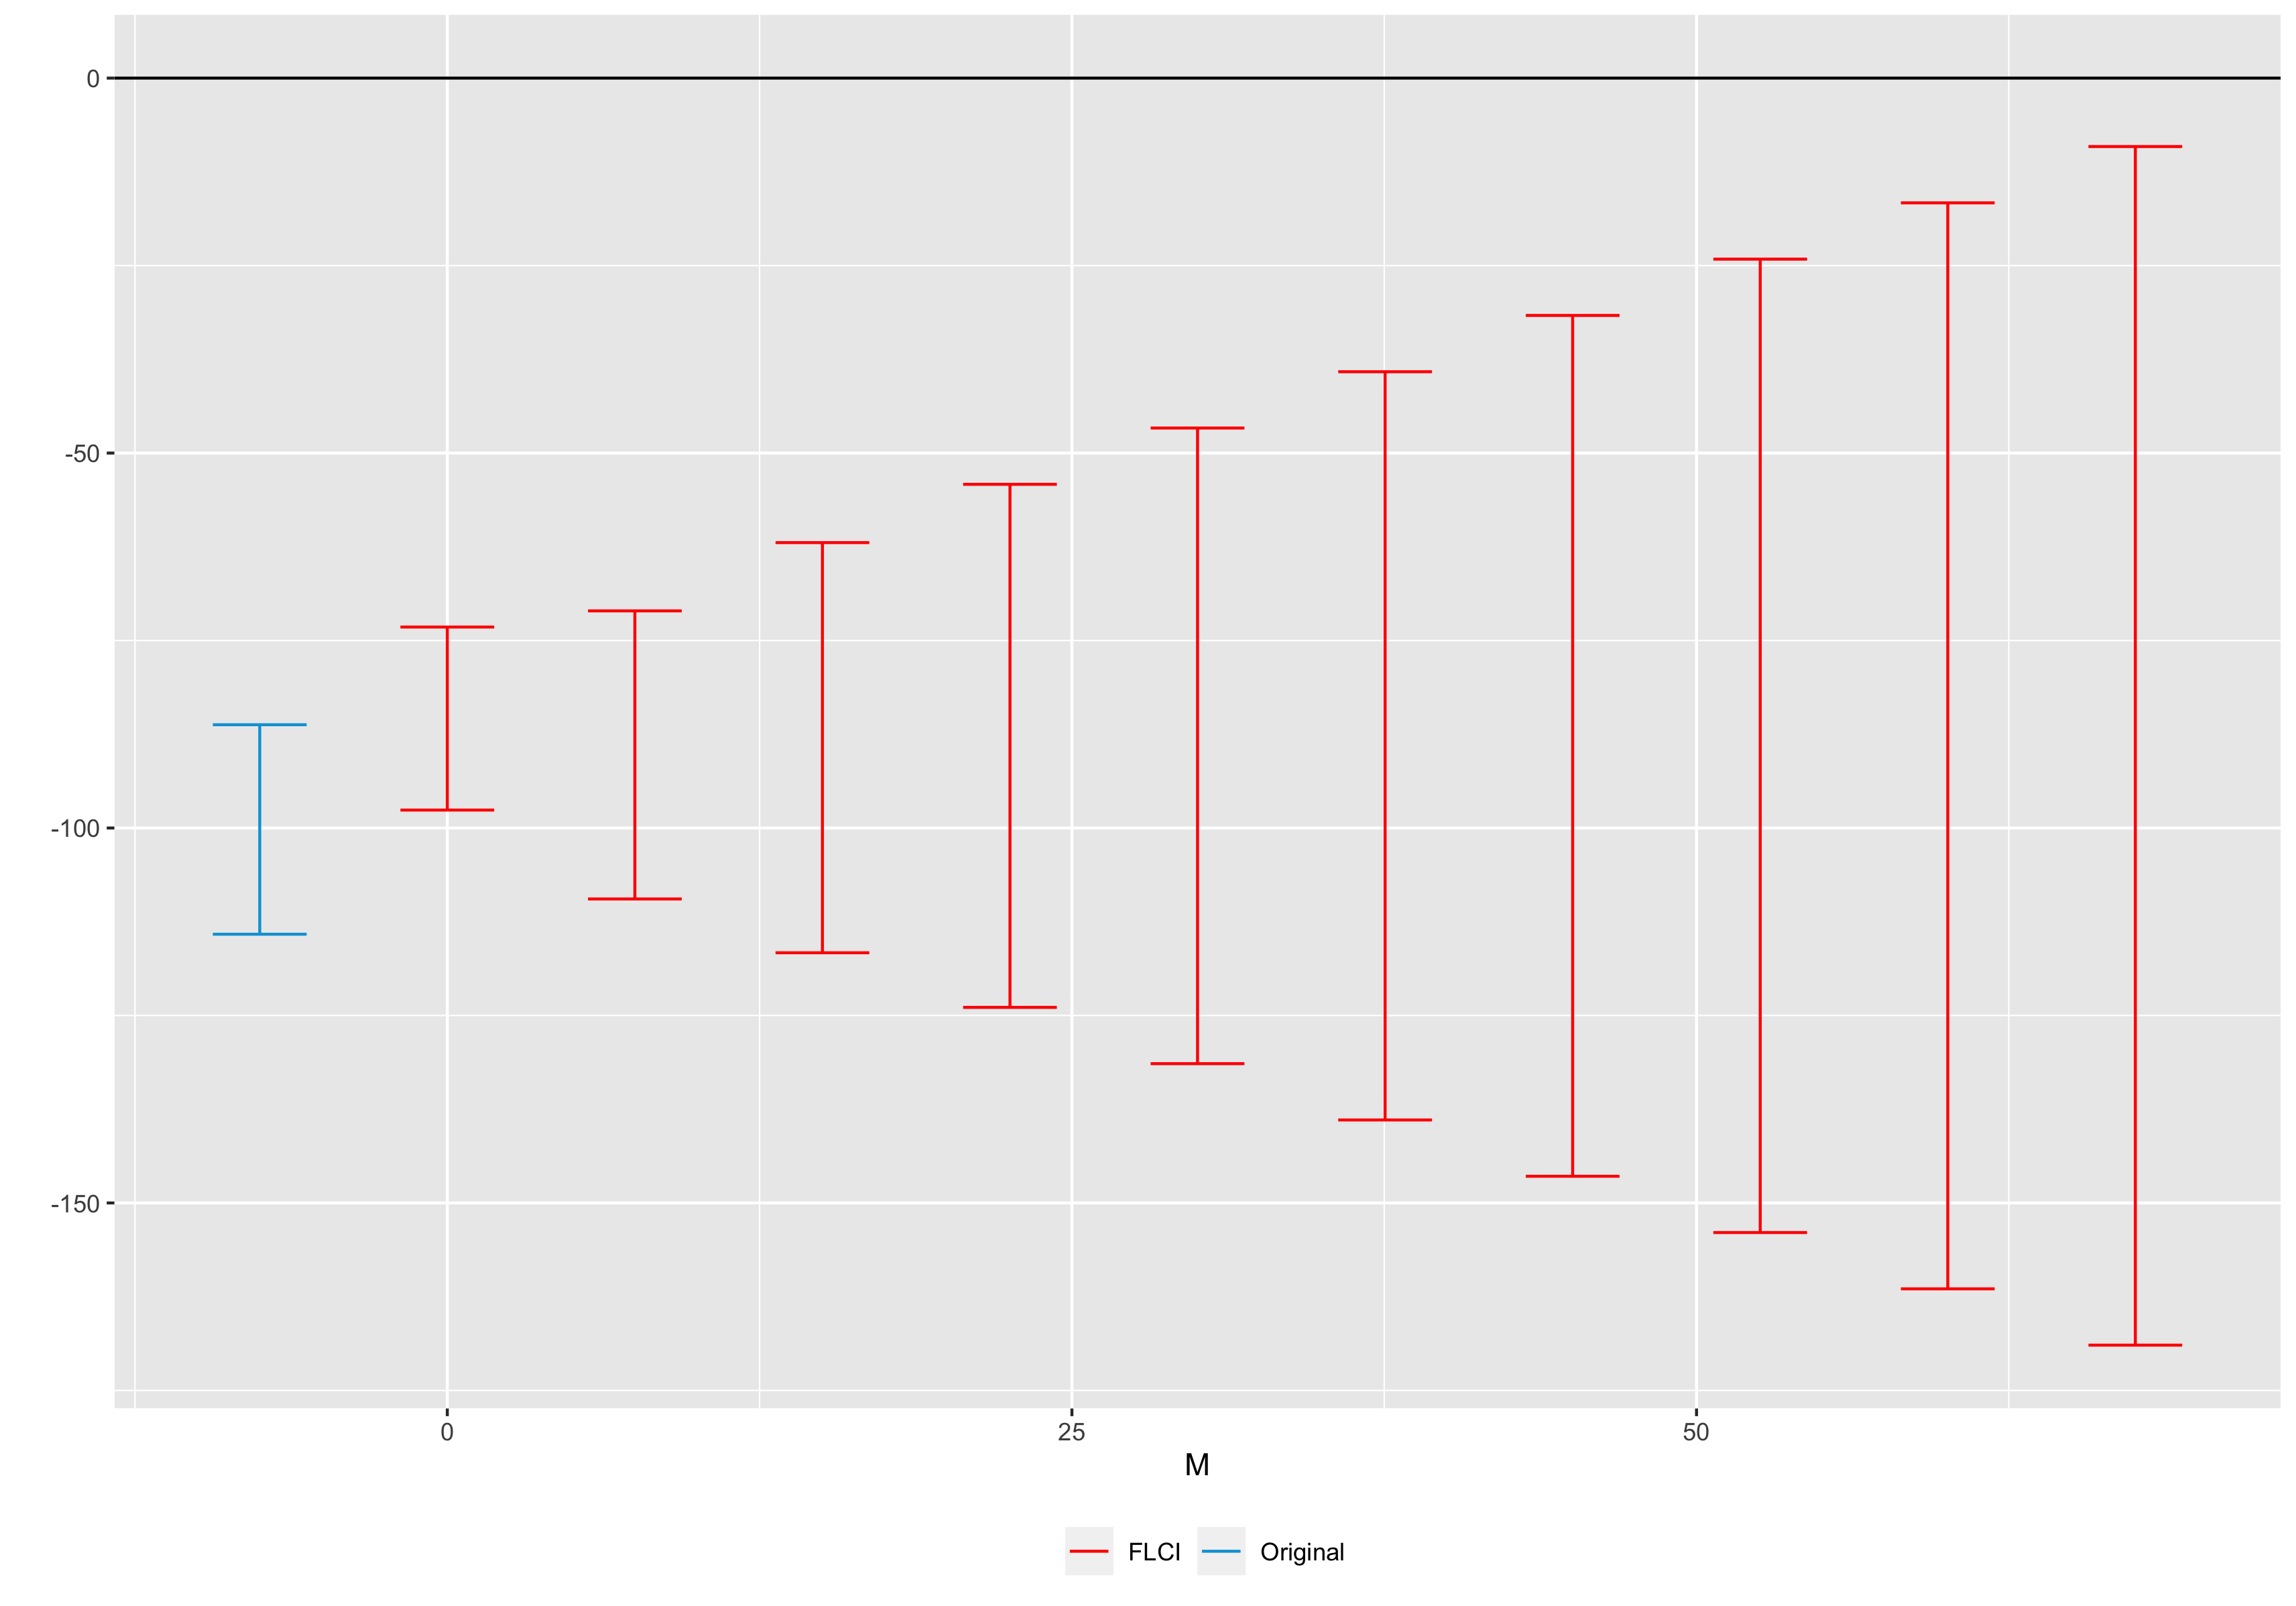
\includegraphics[width=.32\textwidth]{\figdir/cs_hdid_smooth.png}
%     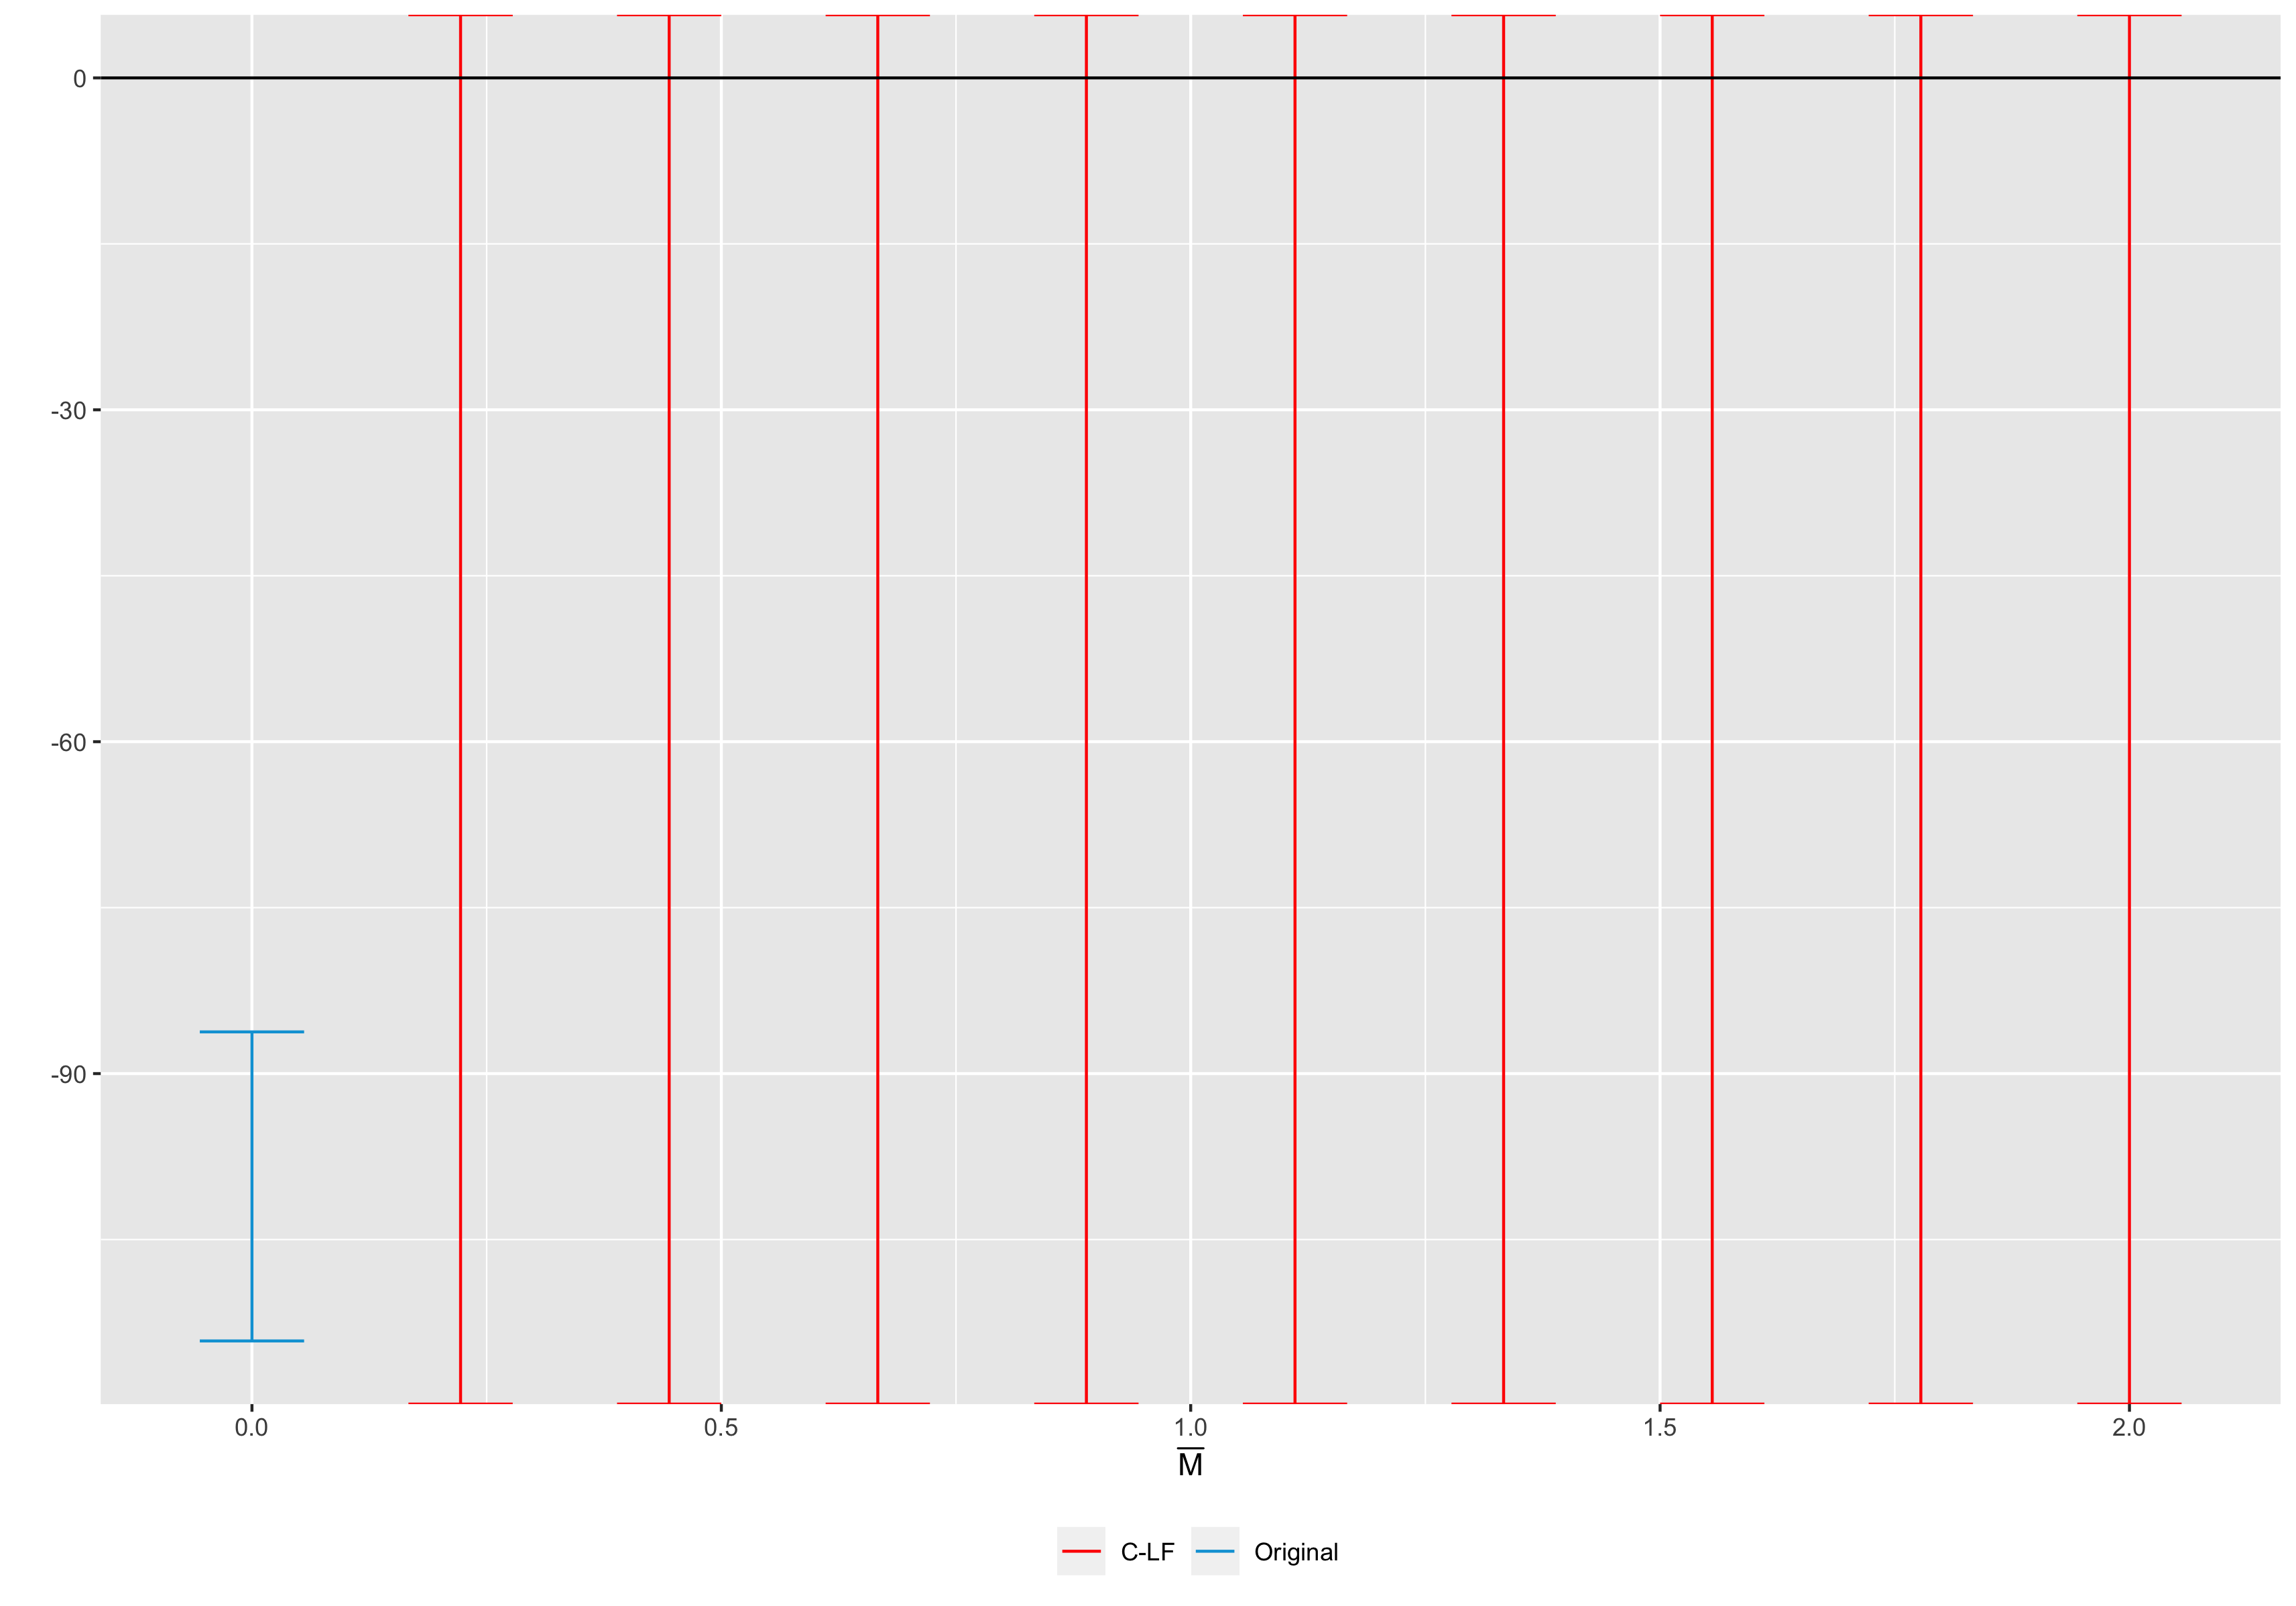
\includegraphics[width=.32\textwidth]{\figdir/cs_hdid_relmag.png}
%     \fignote{\textwidth}{...}
% \end{figure}

